%%%%%%%%%%%%%%%%%%%%%%%%%%%%%%%%%%%%%%%%%%%%%%%%%%%%%%%%%%%%%%%%%%%%%%%%%%%%%%%%
%% Plantilla de memoria en LaTeX para la ETSIT - Universidad Rey Juan Carlos
%%
%% Por Gregorio Robles <grex arroba gsyc.urjc.es>
%%     Grupo de Sistemas y Comunicaciones
%%     Escuela Técnica Superior de Ingenieros de Telecomunicación
%%     Universidad Rey Juan Carlos
%% (muchas ideas tomadas de Internet, colegas del GSyC, antiguos alumnos...
%%  etc. Muchas gracias a todos)
%%
%% La última versión de esta plantilla está siempre disponible en:
%%     https://github.com/gregoriorobles/plantilla-memoria
%%
%% Para obtener PDF, ejecuta en la shell:
%%   make
%% (las imágenes deben ir en PNG o JPG)

%%%%%%%%%%%%%%%%%%%%%%%%%%%%%%%%%%%%%%%%%%%%%%%%%%%%%%%%%%%%%%%%%%%%%%%%%%%%%%%%

\documentclass[a4paper, 17pt]{book}
%\usepackage[T1]{fontenc}

\usepackage[a4paper, left=2.5cm, right=2.5cm, top=3cm, bottom=3cm]{geometry}
\usepackage{times}
\usepackage[utf8]{inputenc}
\usepackage[spanish]{babel} % Comenta esta línea si tu memoria es en inglés
\usepackage{url}
%\usepackage[dvipdfm]{graphicx}
\usepackage{graphicx}
\usepackage{float}  %% H para posicionar figuras
\usepackage[nottoc, notlot, notlof, notindex]{tocbibind} %% Opciones de índice
\usepackage{latexsym}  %% Logo LaTeX

\title{Memoria del Proyecto}
\author{Nombre del autor}

\renewcommand{\baselinestretch}{1.5}  %% Interlineado

\begin{document}

\renewcommand{\refname}{Bibliografía}  %% Renombrando
\renewcommand{\appendixname}{Apéndice}

%%%%%%%%%%%%%%%%%%%%%%%%%%%%%%%%%%%%%%%%%%%%%%%%%%%%%%%%%%%%%%%%%%%%%%%%%%%%%%%%
% PORTADA

\begin{titlepage}
\begin{center}
\begin{tabular}[c]{c c}
%\includegraphics[bb=0 0 194 352, scale=0.25]{logo} &
\includegraphics[scale=0.25]{img/logo_vect.png} &
\begin{tabular}[b]{l}
\Huge
\textsf{UNIVERSIDAD} \\
\Huge
\textsf{REY JUAN CARLOS} \\
\end{tabular}
\\
\end{tabular}

\vspace{3cm}

\Large
ESCUELA TÉCNICA SUPERIOR DE INGENIERÍA INFORMÁTICA
\vspace{0.4cm}

\large
Curso Académico 2019/2020

\vspace{0.8cm}

Proyecto Fin de Máster

\vspace{2.5cm}

\LARGE
IMPLEMENTACIÓN DE UN MOTOR GRÁFICO BASADO EN COMPONENTES

\vspace{4cm}

\large
Autor : Fº Javier Gutiérrez-Maturana Sánchez \\
Tutor : Cristian Rodríguez Bernal
\end{center}
\end{titlepage}

\newpage
\mbox{}
\thispagestyle{empty} % para que no se numere esta pagina


%%%%%%%%%%%%%%%%%%%%%%%%%%%%%%%%%%%%%%%%%%%%%%%%%%%%%%%%%%%%%%%%%%%%%%%%%%%%%%%%
%%%% Para firmar
\clearpage
\pagenumbering{gobble}
\chapter*{}

\vspace{-4cm}
\begin{center}
\LARGE
\textbf{Proyecto Fin de Master}

\vspace{1cm}
\large
Implementación de un motor gráfico basado en componentes

\vspace{1cm}
\large
\textbf{Autor :} Fº Javier Gutierrez-Maturana Sánchez \\
\textbf{Tutor :} Cristian Rodríguez Bernal

\end{center}

\vspace{1cm}
La defensa del presente Proyecto Fin de Master se realizó el día \qquad$\;\,$ de \qquad\qquad\qquad\qquad \newline de 2020, siendo calificada por el siguiente tribunal:


\vspace{0.5cm}
\textbf{Presidente:}

\vspace{1.2cm}
\textbf{Secretario:}

\vspace{1.2cm}
\textbf{Vocal:}


\vspace{1.2cm}
y habiendo obtenido la siguiente calificación:

\vspace{1cm}
\textbf{Calificación:}


\vspace{1cm}
\begin{flushright}
Móstoles, a \qquad$\;\,$ de \qquad\qquad\qquad\qquad de 2020
\end{flushright}

%%%%%%%%%%%%%%%%%%%%%%%%%%%%%%%%%%%%%%%%%%%%%%%%%%%%%%%%%%%%%%%%%%%%%%%%%%%%%%%%
%%%% Dedicatoria

\chapter*{}
\pagenumbering{Roman} % para comenzar la numeracion de paginas en numeros romanos
\begin{flushright}
\textit{Dedicado a \\
Dedicado a mis padres y a mi amigo Nacho y su familia que lo han dado todo y han luchado por mí cuando más lo necesitaba. Gracias.}
\end{flushright}

%%%%%%%%%%%%%%%%%%%%%%%%%%%%%%%%%%%%%%%%%%%%%%%%%%%%%%%%%%%%%%%%%%%%%%%%%%%%%%%%
%%%% Agradecimientos

\chapter*{Agradecimientos}
%\addcontentsline{toc}{chapter}{Agradecimientos} % si queremos que aparezca en el índice
\markboth{AGRADECIMIENTOS}{AGRADECIMIENTOS} % encabezado 

Quería agradecer este trabajo a todas las personas que me han acompañado a lo largo de la 
carrera compañeros y profesores, con los que he aprendido tecnologías punteras que son 
utilizadas en toda la industria actual, a mis padres y mis hermanas y a mi segunda familia
la familia de Nacho que me han dado el último empujon para que decidiera terminar y 
presentar este trabajo.
%%%%%%%%%%%%%%%%%%%%%%%%%%%%%%%%%%%%%%%%%%%%%%%%%%%%%%%%%%%%%%%%%%%%%%%%%%%%%%%%
%%%% Resumen

\chapter*{Resumen}
%\addcontentsline{toc}{chapter}{Resumen} % si queremos que aparezca en el índice
\markboth{RESUMEN}{RESUMEN} % encabezado

Este trabajo está formado por algunas de las características que forman los módulos 
y abstracciones de un motor gráfico para videojuegos y entornos virtuales. Se utilizará 
la librería gráfica de OpenGL y se realizará un desarrollo haciendo uso de algoritmos 
gráficos y un patrón de diseño basado en componentes utilizado en la mayoría de motores
gráficos actuales. 

\vspace{1mm} %5mm vertical space

El motor contará con un árbol de transformadas para gestionar el espacio de coordenadas 
dentro de una escena con objetos en movimiento. La escena contará con objetos de iluminación 
y objetos geométricos con materiales. Los objetos geométricos podrán ser cargados desde el 
propio motor o desde ficheros externos para cargar objetos geométricos más complejos y 
cargar materiales basados en texturas difusas, especulares y normales de manera dinámica. 
El usuario del motor será capaz de cargar escenas animadas haciendo uso de componentes 
externas implementadas en cualquier objeto. Además el motor contará con un conjunto de 
cámaras para poder realizar el renderizado de la escena desde puntos de vista diferentes 
o realizar seguimiento de objetos en la escena y de esta manera tener cámaras de los 
objetos en tercera persona que podrán ser controladas por el usuario. El sistema de 
iluminación contará con luces puntuales, direccionales y focales y el usuario podrá 
definir sus propios materiales para decidir la reacción de las superficies de los 
objetos renderizables a la iluminación definida en la escena. Por último el usuario 
podrá definir controles de teclado para mover las cámaras o los objetos que se encuentran 
dentro de la escena.

%%%%%%%%%%%%%%%%%%%%%%%%%%%%%%%%%%%%%%%%%%%%%%%%%%%%%%%%%%%%%%%%%%%%%%%%%%%%%%%%
%%%% Resumen en inglés

\chapter*{Summary}
%\addcontentsline{toc}{chapter}{Summary} % si queremos que aparezca en el índice
\markboth{SUMMARY}{SUMMARY} % encabezado

This work is formed by some of the characteristics that make up the modules
and abstractions of a graphics engine for video games and virtual environments. It will be used
the OpenGL graphic library and a development will be carried out using algorithms
graphics and a component-based design pattern used in most engines current graphics.

\vspace{1mm} %5mm vertical space

The engine will have a transform tree to manage the coordinate space
within a scene with moving objects. The scene will feature lighting objects
and geometric objects with materials. Geometric objects can be loaded from the
own engine or from external files to load more complex geometric objects and
load materials based on diffuse, specular, and normal textures dynamically.
The user of the engine will be able to load animated scenes using components
external implemented in any object. In addition, the engine will have a set of
cameras to render the scene from different points of view
or track objects in the scene and in this way have cameras of the
third person objects that can be controlled by the user. The system
lighting will have point, directional and focal lights and the user will be able to
define your own materials to decide the reaction of the surfaces of the
Renderable objects to the lighting defined in the scene. Finally the user
You can define keyboard controls to move the cameras or objects that are found
within the scene.

%%%%%%%%%%%%%%%%%%%%%%%%%%%%%%%%%%%%%%%%%%%%%%%%%%%%%%%%%%%%%%%%%%%%%%%%%%%%%%%%
%%%%%%%%%%%%%%%%%%%%%%%%%%%%%%%%%%%%%%%%%%%%%%%%%%%%%%%%%%%%%%%%%%%%%%%%%%%%%%%%
% ÍNDICES %
%%%%%%%%%%%%%%%%%%%%%%%%%%%%%%%%%%%%%%%%%%%%%%%%%%%%%%%%%%%%%%%%%%%%%%%%%%%%%%%%

% Las buenas noticias es que los índices se generan automáticamente.
% Lo único que tienes que hacer es elegir cuáles quieren que se generen,
% y comentar/descomentar esa instrucción de LaTeX.

%%%% Índice de contenidos
\tableofcontents 
%%%% Índice de figuras
\cleardoublepage
%\addcontentsline{toc}{chapter}{Lista de figuras} % para que aparezca en el indice de contenidos
\listoffigures % indice de figuras
%%%% Índice de tablas
%\cleardoublepage
%\addcontentsline{toc}{chapter}{Lista de tablas} % para que aparezca en el indice de contenidos
%\listoftables % indice de tablas


%%%%%%%%%%%%%%%%%%%%%%%%%%%%%%%%%%%%%%%%%%%%%%%%%%%%%%%%%%%%%%%%%%%%%%%%%%%%%%%%
%%%%%%%%%%%%%%%%%%%%%%%%%%%%%%%%%%%%%%%%%%%%%%%%%%%%%%%%%%%%%%%%%%%%%%%%%%%%%%%%
% INTRODUCCIÓN %
%%%%%%%%%%%%%%%%%%%%%%%%%%%%%%%%%%%%%%%%%%%%%%%%%%%%%%%%%%%%%%%%%%%%%%%%%%%%%%%%

\cleardoublepage
\chapter{Introducción}
\label{sec:intro} % etiqueta para poder referenciar luego en el texto con ~\ref{sec:intro}
\pagenumbering{arabic} % para empezar la numeración de página con números

En este capítulo hablaremos sobre el uso de motores gráficos que hacen uso de librerías gráficas 
para realizar el renderizado por pantalla de los objetos a través de los motores gráficos los usuarios 
pueden realizar escenas virtuales añadiendo objetos, luces o animación para desarrollar un entorno 
de realidad virtual, un videojuego, una simulación, una película de animación.

\vspace{1mm} %5mm vertical space

Los motores gráficos facilitan la tarea al desarrollador de generar geometrías o materiales a 
través de programas que se ejecutan dentro de las tarjetas gráficas programas de shaders de esta
manera la computación de los vértices de una geometría se realizan de manera paralela dentro de la GPU.

\vspace{1mm} %5mm vertical space

El uso del patrón de diseño basado en componentes externas ayudará de forma significativa la animación 
de la escena, la generación de eventos temporales y eventos de teclado para la interacción del usuario 
de la aplicación gráfica desarrollada con el motor.

\section{Motivación y contexto}
\label{sec:}

El mercado de los videojuegos está marcado por dos tipos de creadores de videojuegos a, según he podido ir 
viendo a lo largo de mis investigaciones en este campo. Existen usuarios que no tienen conocimientos 
previos o una base sobre ingeniería gráfica que cuentan con grandes ideas o proyectos y necesitan de
ayuda para transcribir sus ideas o mundos dentro de una máquina. 

\vspace{1mm} %5mm vertical space

La otra parte está formada por gente más especializada que cuentan con una base tecnológica en el campo 
de la computación gráfica y generan gran cantidad de herramientas, servicios o plataformas para la 
creación de aplicaciones gráficas de forma sencilla e intuitiva. 

\vspace{1mm} %5mm vertical space

Estos desarrolladores utilizan las librerías gráficas implementadas por los fabricantes de las tarjetas
gráficas o GPUs Graphic Processing Unit y que siguen unos estándares a la hora de realizar los drivers
de las tarjetas, especificados por organizaciones colectivas de empresas en las que se encuentran
gran parte de los fabricantes. 

\vspace{1mm} %5mm vertical space

Actualmente existen diversos motores gráficos en el mercado, siendo los más destacados Unity, Unreal y Blender,
los cuales facilitan a los usuarios el desarrollo de videojuegos y aplicaciones gráficas, así como una gestión
de la memoria y los objetos.

\vspace{1mm} %5mm vertical space

La idea del proyecto es trabajar con las especificaciones gráficas de bajo nivel y ofrecer al usuario un motor
gráfico con conceptos fáciles de entender, herramientas sencillas y ofrecer un buen rendimiento en el
renderizado de las aplicaciones en comparativa con otros motores. 

\vspace{1mm} %5mm vertical space

El problema presentado en la mayoría de motores gráficos es que suelen tener una curva de aprendizaje difícil
de entender para usuarios que no estén familiarizados con el uso de programación gráfica aunque su punto fuerte
suele ser que tienen un buen rendimiento a la hora del desarrollo de las aplicaciones gráficas o su renderizado.

\vspace{1mm} %5mm vertical space

Otros motores sin embargo suelen tener una curva de aprendizaje más fácil de seguir con editores o conceptos más simples,
sin embargo a la hora de medir el rendimiento de estos motores suelen tener un coste computacional más elevado.
La idea de este proyecto es la realización de una plataforma sencilla y con una optimización en el rendimiento de la
plataforma y enseñar los conceptos básicos utilizados en la mayoría de motores gráficos para realizar aplicaciones gráficas.

\vspace{1mm} %5mm vertical space

La decisión de realizar el motor utilizando la librería gráfica de OpenGL 3.3 es la facilidad de puesta en marcha del
entorno, los conocimientos previos de OpenGL obtenidos en asignaturas previas y la facilidad de búsqueda de tutoriales
realizados por la comunidad, al tratarse de una especificación que lleva siendo utilizada desde hace tiempo

\section{Estructura del documento}
\label{sec:estructura}

El documento comienza con un el primer capítulo donde existirá una pequeña introducción de la resolución 
del problema, cómo enfocar un diseño de un motor gráfico basado en componentes y uso de librerías gráficas
para conseguir el objetivo. Existe un apartado de motivación y contexto donde se explica a qué parte del
mercado de los videojuegos está enfocado el proyecto. En el apartado de objetivos se explica una serie de
hitos a conseguir en el proyecto y finalizados de manera correcta, para terminar el capítulo uno, el
apartado de estructura de la memoria define la composición de capítulos del documento.

\vspace{1mm} %5mm vertical space

El segundo capítulo describe las tecnologías utilizadas en el desarrollo del proyecto además de otras
tecnologías a forma de comparativa para explicar las tecnologías utilizadas en el desarrollo y comentar
otros competidores en el desarrollo de motores gráficos y plataformas para el desarrollo de aplicaciones gráficas. 

\vspace{1mm} %5mm vertical space

La arquitectura e implementación del motor gráfico se explica en el capítulo tres, realiza una definición
estática del proyecto donde se podrán ver las técnicas gráficas utilizadas y el patrón de diseño basado en
componentes que forma la estructura principal del motor. La segunda parte del capítulo describe cómo
funciona de forma dinámica el motor, en este apartado se puede ver la interacción del motor con la tarjeta
gráfica y la ejecución del renderizado.

\vspace{1mm} %5mm vertical space

El cuarto capítulo muestra diferentes simulaciones realizadas con el motor y uso de blender para realizar
comparaciones de rendimiento y su facilidad de uso o similitud de ambos motores. Las simulaciones mostrarán
entornos virtuales explicando las técnicas gráficas que soporta el motor y la funcionalidad completa.
Cada simulación resaltará una parte importante de la funcionalidad del motor y su finalización de forma exitosa.
Por último en el capítulo cinco capítulo de conclusiones comentará la valoración final de los objetivos
conseguidos posibles trabajos futuros y cuál ha sido la complejidad del desarrollo.

%% \begin{itemize}
%%  \item En el primer capítulo se hace una intro al proyecto.
  
%%  \item En el capítulo~\ref{chap:objetivos} se muestran los objetivos del proyecto.
  
%%  \item A continuación se presenta el estado del arte.
  
%%  \item \ldots
%% \end{itemize}

%%%%%%%%%%%%%%%%%%%%%%%%%%%%%%%%%%%%%%%%%%%%%%%%%%%%%%%%%%%%%%%%%%%%%%%%%%%%%%%%
%%%%%%%%%%%%%%%%%%%%%%%%%%%%%%%%%%%%%%%%%%%%%%%%%%%%%%%%%%%%%%%%%%%%%%%%%%%%%%%%
% OBJETIVOS %
%%%%%%%%%%%%%%%%%%%%%%%%%%%%%%%%%%%%%%%%%%%%%%%%%%%%%%%%%%%%%%%%%%%%%%%%%%%%%%%%

\cleardoublepage
\chapter{Objetivos}
\label{chap:objetivos}

\section{Objetivo general}
\label{sec:objetivo-general}

En el transcurso del proyecto se determinaron una serie de objetivos o hitos a conseguir dentro del motor gráfico. 
Para realizar el conjunto de objetivos del proyecto se tuvieron en cuenta las abstracciones básicas que forman
un motor gráfico y la realización de animaciones de manera externa y flexible, se realizaron una serie de
subobjetivos que definen los conceptos principales que tienen en común gran parte de motores gráficos.
Las abstracciones utilizadas dentro de los motores gráficos que son comunes en su diseño e implementadas
en el proyecto como subobjetivos se definen a continuación:

\section{Objetivos específicos}
\label{sec:objetivos-especificos}

\begin{itemize}
  \item Creación de una escena para realizar la gestión de un espacio de coordenadas con el uso de
  transformadas para representar una escena animada con diferentes tipos de objetos y movimientos.
  
  \item Definición de materiales a través de programas donde se especificarán las propiedades del
  material ante la iluminación de la escena con el uso de texturas difusas, normales y especulares.
  
  \item Importar ficheros de geometrías para cargar modelos complejos en un formato estandarizado
  y también añadir texturas generando los materiales de la geometría de manera dinámica desde los ficheros.
  
  \item Implementación de un sistema de luces básico para iluminar una escena, haciendo uso de luces
  puntuales, focales, direccionales y un movimiento dinámico de la iluminación.
  
  \item Abstracción del cauce gráfico para el usuario realizando un diseño por etapas del motor
  facilitando la renderización de los objetos geométricos definidos por el usuario.
  
  \item Desarrollar un patrón de diseño basado en componentes para definir el movimiento y
  comportamiento de objetos y diseño del motor. El usuario podrá definir componentes 
  externas en los objetos para generar la animación o comportamientos de los objetos en el renderizado.

\end{itemize}

\section{Planificación temporal}
\label{sec:planificacion-temporal}

En este apartado se especifica las tareas a realizar durante el proyecto el tiempo utilizado para el desarrollo de cada una 
de las funcionalidades del motor, especificado en un diagrama de grant por sprints de trabajo. 

\begin{figure}[H]
    \centering
    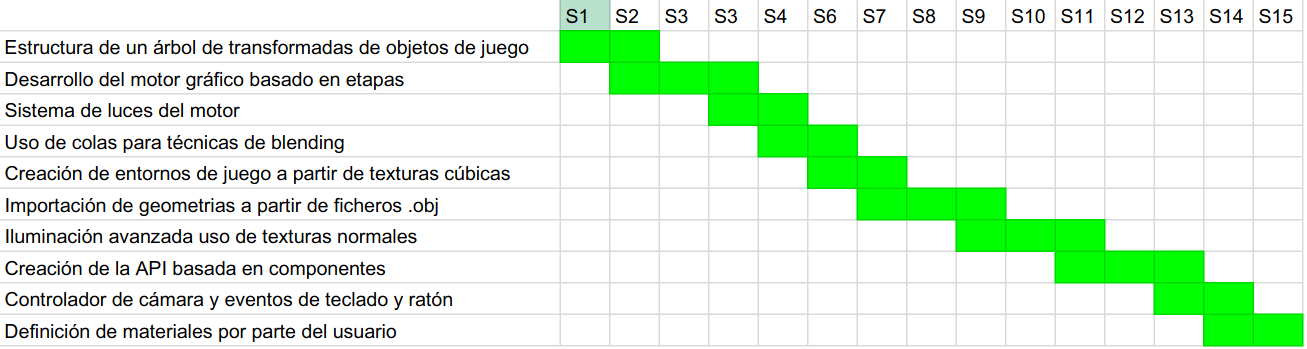
\includegraphics[scale=0.35, keepaspectratio]{img/Schedule.png}
    \caption{Diagrama de grant de la planifiación temporal del proyecto}
    \label{figura:khronos}
\end{figure}

El diagrama muestra el tiempo utilizado para cada sub tarea del proyecto, con el uso de las subtareas se simplifica el 
desarrollo general. Las columnas indican un sprint que equivale en nuestro caso a una semana de trabajo. Cada semana
está planificada por 40 horas de trabajo, por tanto la cantidad total de horas invertidas en el proyecto consta de:

\begin{equation} Planificacion_{horas} = NSprints \cdot 40_{horas} = 600_{horas} \end{equation}

El trabajo tiene una estimación de tiempo total de 600 horas dedicando el tiempo necesario a cada uno de los sub
objetivos pudiéndose alargar en caso de que se encuentren dificultades a la hora de la implementación. Esta es una
estimación apróximada del alumno dónde según su criterio ha indicado un mayor número de Sprints
a las tareas con una mayor complejidad de desarrollo.

%%%%%%%%%%%%%%%%%%%%%%%%%%%%%%%%%%%%%%%%%%%%%%%%%%%%%%%%%%%%%%%%%%%%%%%%%%%%%%%%
%%%%%%%%%%%%%%%%%%%%%%%%%%%%%%%%%%%%%%%%%%%%%%%%%%%%%%%%%%%%%%%%%%%%%%%%%%%%%%%%
% ESTADO DEL ARTE %
%%%%%%%%%%%%%%%%%%%%%%%%%%%%%%%%%%%%%%%%%%%%%%%%%%%%%%%%%%%%%%%%%%%%%%%%%%%%%%%%

\cleardoublepage
\chapter{Antecedentes y estado del arte}

En este apartado se hablará de tecnologías utilizadas en el proyecto relacionadas con el campo de investigación
computacional de HPG High Performance Graphics. 

\vspace{1mm} %5mm vertical space

Primero se hablará de cual es concepto de High Performance Graphics dando una introducción a en qué
campo de investigación están basadas las tecnologías del proyecto, después se hablará de las tecnologías
y otras similares para realizar comparativas y justificar las utilizadas, como parte final se dará una
breve introducción de otros motores gráficos que hacen uso de estas tecnologías, mismos patrones de diseño y modularización.

\section{Concepto de rendimiento gráfico de altas prestaciones} 
\label{sec:HPG}

High Performance Graphics (HPG) está compuesto por un foro internacional de investigación de sistemas gráficos
orientados al rendimiento y utilización de algoritmos innovadores, implementaciones eficientes de arquitecturas
de hardware orientadas a la computación gráfica de las máquinas. 

\vspace{1mm} %5mm vertical space

Los ingenieros e investigadores realizan conferencias sobre los algoritmos su eficiencia y el diseño de nuevo
hardware orientado a gráficos. Las compañías especializadas en este sector de la industria de las TIC’s, discuten
entre ellos las complejas interacciones entre el hardware masivamente paralelo, modelos de programación novedosos
y algoritmos gráficos eficientes para realizar nuevas implementaciones de librerías gráficas que harán uso otros
desarrolladores.

\vspace{1mm} %5mm vertical space

Dentro de esta sección se comentará las diferentes API’s gráficas que se utilizan de forma masiva en la industria:
Vulkan, DirectX y OpenGL. Para acabar en la sección de antecedentes se explicarán algunos de los motores gráficos
más utilizados en la actualidad y algunas de las características comunes con el motor gráfico desarrollado.

\section{Grupo Khronos} 
\label{sec:Grupo Khronos}

El grupo Khronos es una comunidad abierta, que cuenta con más de 140 compañías hardware y software que crean los estándares de
aceleración avanzados para gráficos 3D realidad aumentada o aprendizaje automático. Los estándares de Khronos incluyen las
siguientes especificaciones.  Vulkan®, OpenGL®, OpenGL® ES, OpenGL® SC, WebGL ™, SPIR-V ™, OpenCL ™, SYCL ™, OpenVX ™,
NNEF ™, COLLADA ™, OpenXR ™, 3D Commerce ™ y glTF ™. 

\vspace{1mm} %5mm vertical space

Los miembros de la comunidad de Khronos pueden contribuir al desarrollo de las especificaciones y votar en las etapas de
desarrollo antes del despliegue al público y pueden acelerar el desarrollo de sus plataformas a través del acceso a
borradores de las especificaciones antes de su salida.

\begin{figure}[H]
    \centering
    
\includegraphics[width=9cm, keepaspectratio]{img/khronos.jpg}
    \caption{Logotipo del grupo khronos.}
    \label{figura:khronos}
\end{figure}

Las compañías pueden usar la especificación del estándar de las librerías de Khronos pero la API debe probarse y pasar un
conjunto de tests del estándar. Si la implementación supera con éxito las pruebas del estándar el grupo khronos da por
buena la especificación de la API en calidad y compatibilidad con el estándar para el fabricante del hardware.
La necesidad de realizar un estándar en el desarrollo de tecnologías HPG es necesaria para que todos los fabricantes
sigan unas normas a la hora de diseñar su hardware o software y que puedan ser compatibles con el software gráfico a la
hora de salir al mercado. 

\vspace{1mm} %5mm vertical space

La tarea del grupo Khronos es especificar estos estándares a todos los diseñadores de software y hardware. El uso del
estándar abstrae al usuario del sistema operativo a la hora de realizar el desarrollo de aplicaciones gráficas usando
la interfaz de la librería de manera directa con el driver que implementa el estándar, sin tener que usar la interfaz
con el sistema operativo de la máquina. 

\vspace{1mm} %5mm vertical space

El grupo Khronos cuenta con especificaciones de librerías gráficas que cubren la aceleración de gráficos desde sistemas
móviles tablets, sistemas embebidos a supercomputadores y ordenadores de sobremesa o consolas, cada una de estas
especificaciones está centrada en un tipo de máquina o un subconjunto de ellas. Algunas de las especificaciones del grupo
Khronos conocidas son OpenGL y Vulkan. Las últimas versiones de estos dos estándares son OpenGL 4.0 y Vulkan 1.2. 

\vspace{1mm} %5mm vertical space

Primero se explicará la librería gráfica de Vulkan, seguida de la especificación gráfica de Microsoft DirectX en su última
versión y por último se hablará en detalle de OpenGL 3.3, librería gráfica utilizada en la implementación del motor.

\section{Vulkan} 
\label{sec:Vulkan}

Vulkan está diseñada como una interfaz software de comunicación entre el hardware y las capas software de alto nivel para
realizar aplicaciones gráficas. El objetivo principal de Vulkan es implementar una especificación de librería gráfica
especificada por el grupo Khronos definiendo funcionalidades y diseño de la implementación.

\subsection{Introducción a Vulkan} 
\label{subsec:IntroVulkan}

Al igual que las APIs de gráficos anteriores, Vulkan está diseñado como una abstracción multiplataforma sobre GPU.
El problema con la mayoría de estas APIs es que la era en la que se diseñaron presentaba hardware de gráficos que se
limitaba principalmente a la funcionalidad fija configurable. Los programadores tenían que proporcionar los datos de
vértice en un formato estándar y estaban a merced de los fabricantes de GPU con respecto a las opciones de iluminación,
sombreado y renderizado.

\vspace{1mm} %5mm vertical space

A medida que maduraban las arquitecturas de las tarjetas gráficas, comenzaron a ofrecer más y más funcionalidades
programables. Toda esta nueva funcionalidad tuvo que integrarse de alguna manera con las APIs existentes. Esto resultó
en abstracciones menos que ideales y muchas conjeturas en el lado del controlador de gráficos para asignar la intención
del programador a las arquitecturas gráficas modernas. Es por eso que hay tantas actualizaciones de controladores para
mejorar el rendimiento en los juegos. Debido a la complejidad de estos controladores, los desarrolladores de aplicaciones
también deben lidiar con inconsistencias entre los proveedores, como la sintaxis que se acepta para los programas de
shaders o sombreado. 

\vspace{1mm} %5mm vertical space

Además de estas nuevas características, la década pasada también vio una afluencia de dispositivos móviles con hardware
de gráficos potente. Estas GPU móviles tienen arquitecturas diferentes en función de sus requisitos de energía y espacio.
Un ejemplo de ello es la representación en mosaico, que se beneficiaría de un rendimiento mejorado al ofrecer al
programador más control sobre esta funcionalidad. Otra limitación que se origina a partir de la antigüedad de estas API
es la compatibilidad limitada de múltiples subprocesos, que puede provocar un cuello de botella en el lado de la CPU.

\vspace{1mm} %5mm vertical space

Vulkan resuelve estos problemas al ser diseñado desde cero para arquitecturas gráficas modernas. Reduce la sobrecarga
del controlador al permitir que los programadores especifiquen claramente su intención utilizando una API más detallada,
y permite que múltiples hilos creen y envíen comandos de forma paralela. La idea detrás de la API es realizar drivers
sencillos de GPUs que sean compatibles con la especificación y aprovechen al máximo las capacidades de hardware paralelamente
masivo actual.

\subsubsection{Capas de Validación} 
\label{subsec:CapsVulkan}

Como se mencionó anteriormente, Vulkan está diseñado para un alto rendimiento y una baja sobrecarga del controlador.
Por lo tanto, incluirá capacidades muy limitadas de verificación y depuración de errores de forma predeterminada.
El controlador a menudo fallará en lugar de devolver un código de error si hace algo mal, o peor aún, parecerá que
funciona en la tarjeta gráfica y fallará por completo en los demás controladores.
Vulkan permite habilitar extensas comprobaciones a través de una función conocida como capas de validación.
Las capas de validación son piezas de código que se pueden insertar entre la API y el controlador de gráficos
para hacer cosas como ejecutar comprobaciones adicionales en los parámetros de función y rastrear problemas
de gestión de memoria. Lo bueno es que puede habilitarse durante el desarrollo y luego deshabilitarlos por
completo al lanzar la aplicación con cero sobrecarga. Cualquiera puede escribir sus propias capas de validación,
pero el Vulkan SDK de LunarG proporciona un conjunto estándar de capas de validación. También debe registrarse
una función de devolución de llamada para recibir mensajes de depuración de las capas.
Debido a que Vulkan es tan explícito sobre cada operación y las capas de validación son tan extensas, en realidad
puede ser mucho más fácil descubrir por qué la pantalla es negra en comparación con OpenGL y Direct3D.

\subsection{El cauce gráfico del Vulkan} 
\label{subsec:CauceVulkan}

El cauce gráfico es la secuencia de operaciones que llevan los vértices y las texturas de sus mallas en 3D hasta
los píxeles en los objetivos de renderizado por pantalla. A continuación se muestra una descripción general
simplificada del cauce gráfico en Vulkan.

\begin{figure}[H]
    \centering
    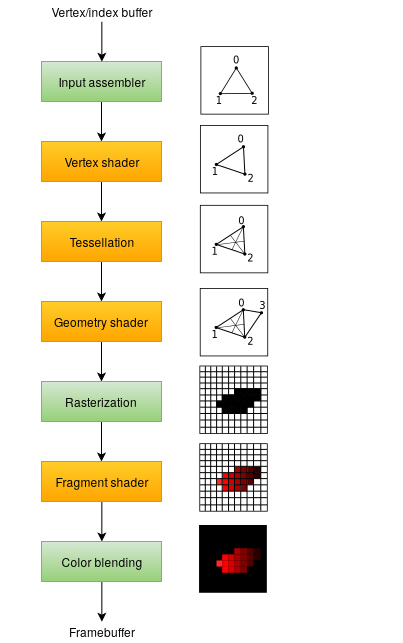
\includegraphics[scale=0.5, keepaspectratio]{img/vulkan_simplified_pipeline.png}
    \caption{Diagrama del cauce gráfico en Vulkan con las etapas principales del cauce,
    las etapas amarillas son programables, las etapas verdes son únicamente configurables
    dentro del cauce de renderizado.}
    \label{figura:khronos}
\end{figure}

A continuación se explican las diferentes etapas mostradas en la imagen del cauce gráfico de Vulkan
y en la parte final de la definición del cauce gráfico se explicará el uso de las etapas programables
y las etapas de configuración.

\begin{itemize}
  \item El ensamblador de entrada recopila los datos de vértices sin procesar de los búferes que
  se especifiquen y también puede usar un búfer de índice para repetir ciertos elementos sin tener
  que duplicar los datos del vértices.
  
  \item El sombreador de vértices se ejecuta para cada vértice y generalmente aplica transformaciones
  para convertir las posiciones de vértice del espacio modelo al espacio de la pantalla. También pasa
  datos de vértices por el pipeline.

  \item Los sombreadores de teselación permiten subdividir la geometría según ciertas reglas para aumentar
  la calidad de la malla. Esto se usa a menudo para hacer que las superficies como las paredes de ladrillo
  y las escaleras se vean menos planas cuando están cerca.

  \item El sombreador de geometría se ejecuta en todas las primitivas (triángulo, línea, punto) y puede
  descartar o generar más primitivas que las que se ingresaron, mapa 1:n. Esto es similar al shader de teselación,
  pero mucho más flexible. Sin embargo, no se usa mucho en las aplicaciones actuales porque el rendimiento no es
  tan bueno en la mayoría de las tarjetas gráficas, excepto en las GPU integradas de Intel.

  \item La etapa de rasterización discretiza las primitivas en fragmentos. Estos son los elementos de píxel
  que rellenan en el framebuffer. Los fragmentos que quedan fuera de la pantalla se descartan y los atributos
  generados por el shader de vértices se interpolan a través de los fragmentos, como se muestra en la figura.
  Por lo general, los fragmentos que están detrás de otros fragmentos de otras primitivas también se descartan
  aquí debido a los tests de profundidad.

  \item El sombreador de fragmentos se invoca para cada fragmento que sobrevive y determina en qué framebuffer (s)
  se escriben los fragmentos y con qué valores de color y profundidad. Puede hacerse utilizando los datos interpolados 
  del shader de vértices, que pueden incluir elementos como coordenadas de textura y normales para la iluminación.

  \item La etapa de mezcla de colores aplica operaciones para mezclar diferentes fragmentos que se asignan al mismo píxel
  en el framebuffer. Los fragmentos pueden simplemente sobrescribirse entre sí, sumarse o mezclarse en función de la transparencia.

\end{itemize}

Las etapas de función fija permiten ajustar las operaciones utilizando parámetros, pero la forma en que funcionan está predefinida.
Las etapas programables pueden cargar código en la tarjeta gráfica para aplicar exactamente las operaciones que se deseen y
optimizar las operaciones en los recursos de la tarjeta.  La etapa de sombreadores de fragmentos, por ejemplo, utiliza esta
clase de programas para implementar desde texturizado e iluminación, para dar un valor final de color de los fragmentos.
Estos programas se ejecutan en muchos núcleos de GPU simultáneamente para procesar muchos objetos y su conjunto de vértices
y fragmentos en paralelo.

\vspace{1mm} %5mm vertical space

El pipeline (procesamiento en serie) de gráficos en Vulkan es casi completamente inmutable, por lo que debe recrearse el
pipeline desde cero si se desea cambiar los sombreados o enlazar diferentes framebuffers. La desventaja es que se deben
crear varios pipelines que representen todas las diferentes combinaciones de estados que se desean usar en las operaciones
de renderizado, sin embargo, debido a que todas las operaciones que se realizan en el pipeline se conocen de antemano,
el driver puede optimizar el renderizado mucho mejor.

\vspace{1mm} %5mm vertical space

Algunas de las etapas programables son opcionales en función de lo que pretende hacer. Por ejemplo, las etapas de
teselación y geometría se pueden deshabilitar si solo se está dibujando una geometría simple. Si solo interesan
los valores de profundidad se puede deshabilitar la etapa de sombreado de fragmentos, que es útil para la generación
de mapas de sombras.

\subsubsection{Operaciones con Vulkan} 
\label{subsubsec:OpVulkan}

La API facilita el trabajo del driver y pone el control del hardware en manos del desarrollador, por ejemplo,
en la sincronización y la gestión de la memoria. Una de las ventajas de Vulkan frente a otras librerías gráficas
es su capacidad para depuración de los programas que se ejecutan en la tarjeta gráfica facilitando y agilizando
el desarrollo de las aplicaciones y la abstracción al desarrollador del hardware y los drivers con los que esté
trabajando. La arquitectura de Vulkan está desarrollada por capas y las herramientas de desarrollo son concebidas
como capas de la API. Grandes compañías de videojuegos como Valve o ID Software están utilizando esta librería
para el desarrollo de sus videojuegos. Es apreciable el aumento del rendimiento para un mismo hardware y una misma
aplicación haciendo uso de esta librería gráfica en lugar de otras especificaciones. 

\vspace{1mm} %5mm vertical space

En la versión de Vulkan 1.1 se han añadido funcionalidades para protección de memoria restricciones de copia de
recursos en el renderizado y protección de contenido multimedia o procesamiento de imagen, además de ofrecer
un conjunto de operaciones paralelas de forma nativa en las etapas de shaders del cauce gráfico. Con estas nuevas
operaciones paralelas se consiguen nuevas formas de comunicación y compartición de memoria al realizar las operaciones
en la GPU de forma paralela.

\begin{figure}[H]
    \centering
    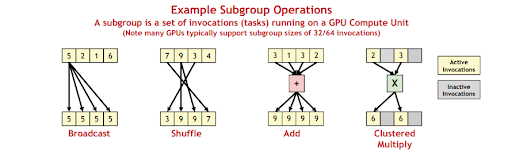
\includegraphics[scale=0.75, keepaspectratio]{img/vulkan_op.png}
    \caption{Imagen de grupo khronos de las operaciones paralelas soportadas de forma nativa en el lenguaje de shaders de Vulkan.}
    \label{figura:khronos}
\end{figure}

En la especificación de Vulkan se pueden encontrar el uso de vistas múltiples y realizar una única renderización
para el uso de múltiples pantallas.


\begin{itemize}
  \item Se puede hacer uso de grupos de dispositivos hardware heterogéneos de fabricantes diferentes que
  funcionan con un driver con Vulkan y mantienen de forma transparente los dispositivos al usuario de las tarjetas.
  
  \item Vulkan cuenta con funcionalidades de computación avanzada, fragmentos de memoria en 2 bytes, restricciones en
  los punteros a estructura de datos en memoria de la GPU y soporte para el desarrollo de núcleos aislados de
  procesamiento dentro del propio hardware.

  \item La especificación de Vulkan también es compatible con el programa de shaders de la librería gráfica de Microsoft
  HLSL, facilitando la portabilidad de un desarrollo hecho en Vulkan a DirectX 12.

  \item El lenguaje de shaders utilizado en Vulkan es SPIR-V y ofrece facilidades para la portabilidad de código escrito
  en SPIR-V a GLSL o HLSL para ser compatible tanto con OpenGL como con DirectX 12 facilitando la portabilidad de las
  aplicaciones y obtener shaders utilizando las mismas funcionalidades gráficas a un lengauje de programación de
  shaders HLSL o GLSL a SPIR-V.  Este trabajo de portabilidad de los lenguajes de shaders se hace a través del
  compilador de SPIR-V que es capaz de traducir de un lenguaje de shaders a otro HLSL, GLSL o SPIR-V. 
  
\end{itemize}

La especificación como todas la especificaciones de librerías gráficas del grupo Khronos está definida en la documentación
del estándar definiendo de forma explícita las funcionalidades obligatorias que deben de tener los fabricantes de las tarjetas
para poder cumplir con el estándar.


\subsection{Sistema de coordenadas en Vulkan} 
\label{subsec:SysVulkan}

Vulkan introduce una serie de cambios interesantes sobre OpenGL con algunos de los cambios clave de rendimiento y flexibilidad
que se mencionan. Un cambio más sutil pero igualmente importante para ser entendido es el del sistema de coordenadas.

\begin{figure}[H]
    \centering
    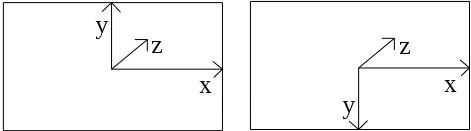
\includegraphics[scale=0.75, keepaspectratio]{img/coordinateDiagram.png}
    \caption{Cambio del sistema de coordenadas de OpenGL a la derecha al de Vulkan en la parte izquierda.}
    \label{figura:khronos}
\end{figure}

El primer cambio importante es que el eje y ahora apunta hacia abajo en la pantalla. Los ejes xz apuntan en la misma
dirección que antes. Esto significa que si no se corrige esto en los shaders portados de GLSL a SPIR-V sucederán dos
cosas importantes. En primer lugar, las imágenes se voltearán, hay múltiples formas de resolver esto. El método
utilizado en las muestras es simplemente agregar la siguiente línea a todos los programas de shaders vértices.

\begin{equation}
gl_Position.y = -gl_Position.y
\end{equation}

En OpenGL teníamos un espacio NDC a la izquierda, en Vulkan tenemos un espacio NDC a la derecha (suponiendo que el valor
de profundidad libre es 1, la función de profundidad es). \begin{equation} GL_LEQUAL / VK_COMPARE_OP_LESS_OR_EQUAL \end{equation}

\vspace{1mm} %5mm vertical space

El otro cambio en el sistema de coordenadas es el eje z, es decir, el rango de profundidad. En OpenGL el valor de profundidad
es un valor absoluto en un rango de [0, 1]. En Vulkan cambia a un valor relativo al vértice más lejano dentro de la ventana.
Para solucionar este problema y obtener los valores absolutos para etapas de face culling se utiliza la siguiente de línea
en la etapa de vértices de SPIR-V en Vulkan. 

\begin{equation}
gl_Position.z = (gl_Position.z + gl_Position.w) / 2.0
\end{equation}

Los trabajos futuros de esta especificación es seguir realizando herramientas de pruebas de calidad de la especificación
y priorizar las necesidades de los desarrolladores gráficos y conducir las nuevas tecnologías de futuras
generaciones de GPUs.

\section{DirectX} 
\label{sec:DirectX}

DirectX es la especificación de la librería gráfica de Microsoft de gráficos 2D y 3D. Esta especificación trata de realizar
una interfaz común para el trabajo en un sistema operativo de Microsoft, teniendo en cuenta la heterogeneidad del hardware de GPUs.

\subsection{Introducción a DirectX} 
\label{subsec:IntroDirectX}

Microsoft lanza su propia especificación para que los fabricantes puedan vender sus tarjetas gráficas en sistemas operativos Windows
implementando la especificación de DirectX en el driver de sus tarjetas gráficas. Microsoft realiza la especificación teniendo en
cuenta las tecnologías de las nuevas generaciones de GPUs que aparecen en el mercado, añadiendo nuevas funcionalidades en la
especificación de la librería, actualmente la versión más reciente de la especificación es la DirectX 12 compatible con la
especificación Vulkan del grupo Khronos.

\vspace{1mm} %5mm vertical space

La tecnología de DirectX está pensada como un conjunto de API’s y cada una de ellas se encarga de realizar un trabajo
independiente de computación gráfica. La librería DirectX Math se encarga de realizar las operaciones matemáticas
sobre vectores o matrices de coma flotante. Las librerías Direct2D y Direct3D se encargan de realizar las renderizaciones
de modelos de gráficos en 2D y 3D respectivamente. También existen librerías para realizar programas compatibles con
versiones antiguas de Windows o hardware que no soporta la nueva especificación de la librería gráfica Classic DirectX
Graphics. Por otro lado Microsoft ha desarrollado una API específica para la entrada de dispositivos en este caso para su
mando de la XBox, XInput y una librería para procesamiento de señales de audio XAudio2. Además cuenta con una librería
de herramientas para depuración diagnóstico y compilación de su lenguaje de shaders HLSL.

\subsection{Sistema de coordenadas en Direct3D} 
\label{subsec:SysDirectX}

Direct3D utiliza un sistema de coordenadas levógiro. Si se están realizando acciones de transformación de una aplicación 
basada en un sistema de coordenadas dextrógiro, se debe realizar dos cambios en los datos pasados de Direct3D de las
geometrías y operaciones de rotación o traslación.

\begin{figure}[H]
    \centering
    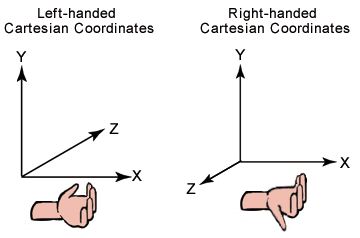
\includegraphics[scale=0.50, keepaspectratio]{img/leftrght.png}
    \caption{Uso de sistema de coordenadas levógiro y dextrógiro. Direct3D hace uso del primero como sistema de coordenadas.}
    \label{figura:khronos}
\end{figure}

Direct3D utiliza tres transformaciones para cambiar las coordenadas de un modelo 3D en coordenadas de píxeles (espacio de pantalla).
Estas transformaciones son transformaciones del mundo, transformaciones de vista y transformaciones de proyección.

\begin{itemize}
  \item La etapa de world transformation controla cómo las coordenadas del modelo se transforman en coordenadas absolutas.
  La etapa transformation world puede incluir traslaciones, rotaciones y escalas, pero no se aplica a las luces.
  
  \item La etapa de view transformation controla la transición de las coordenadas absolutas al "espacio de la cámara",
  determinando la posición de la cámara en el mundo.

  \item La etapa projection transform cambia la geometría del espacio de la cámara al "espacio de clip" y aplica
  distorsión de perspectiva. El término "espacio de clip" se refiere a cómo se recorta la geometría al volumen
  de la vista durante esta transformación descartando las primitivas de la geometría que no son visibles.
  
\end{itemize}

Finalmente, la geometría en el espacio del clip se transforma en coordenadas de píxeles (espacio de pantalla).
Esta transformación está controlada por la configuración de la ventana gráfica.

\begin{figure}[H]
    \centering
    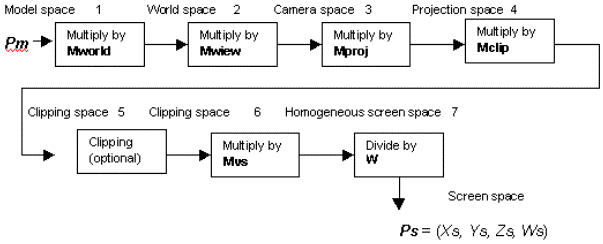
\includegraphics[scale=0.40, keepaspectratio]{img/d3dxfrm61.png}
    \caption{Etapas de transformación de los vértices en el cauce gráfico de OpenGL hasta la coordenada final
    del pixel de renderizado de la geometría por pantalla}
    \label{figura:khronos}
\end{figure}

La etapa de recorte de vértices y las etapas de transformación deben tener lugar en un espacio homogéneo (simplemente,
espacio en el que el sistema de coordenadas incluye un cuarto elemento), pero el resultado final para la mayoría de
las aplicaciones debe ser coordenadas tridimensionales (3D) no homogéneas definidas en el espacio de "pantalla".
Esto significa que tanto los vértices de entrada como la geometría de recorte deben traducirse en un espacio homogéneo
para realizar el recorte o clipping y luego volver a traducirse en un espacio no homogéneo para su visualización.

\subsection{Cauce gráfico en Direct3D 12} 
\label{subsec:CauceDX12}

El cauce gráfico programable Direct3D 12 aumenta significativamente el rendimiento de renderizado en comparación
con las interfaces de programación gráfica de la generación anterior.

\begin{figure}[H]
    \centering
    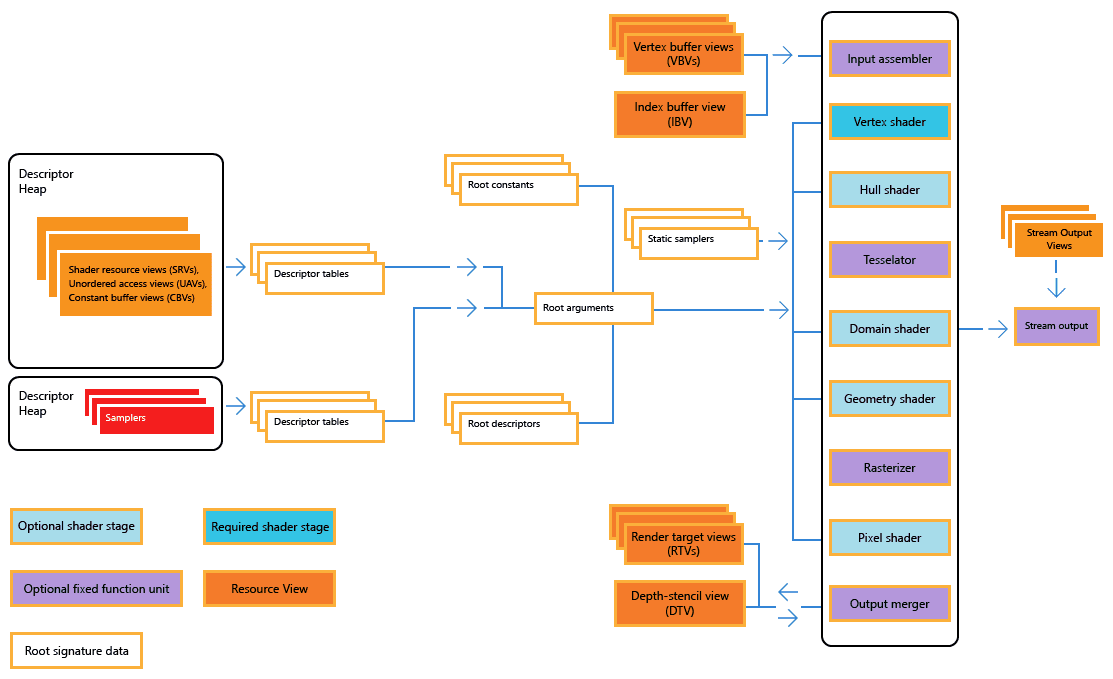
\includegraphics[scale=0.40, keepaspectratio]{img/pipelined123d.png}
    \caption{Diagrama de ilustración del cauce gráfico y estado de los gráficos en Direct3D 12.}
    \label{figura:khronos}
\end{figure}

Un cauce gráfico es un flujo secuencial de entradas y salidas de datos a medida que la GPU procesa los datos.
Dado el estado de la tubería y las entradas, la GPU realiza una serie de operaciones para crear las imágenes resultantes.
Una canalización de gráficos contiene shaders, que realizan cálculos y efectos de representación programables, y operaciones
de funciones fijas. Algunas operaciones del cauce son configurables. 

\vspace{1mm} %5mm vertical space

Una de las diferencias de DirectX 12 respecto a versiones anteriores es el uso de PSO objetos de estado en lugar de la
máquina de estados global del cauce gráfico para guardar el contexto.

\subsubsection{Cauce gráfico con objetos con estado PSO} 
\label{subsubsec:PSO}

Direct3D 12 presenta el objeto de estado de canalización (PSO). En lugar de almacenar y representar el estado del pipeline
en una gran cantidad de objetos de alto nivel, los estados de los componentes de la tubería como el ensamblador de entrada,
el rasterizador, el sombreador de píxeles y la fusión de salida se almacenan en un PSO. Un PSO es un objeto de estado de
canalización unificado que es inmutable después de la creación. 

\vspace{1mm} %5mm vertical space

El PSO seleccionado actualmente se puede cambiar de forma rápida y dinámica, y el hardware y los controladores pueden
convertir directamente un PSO en instrucciones de hardware y estado nativo, preparando la GPU para el procesamiento
de gráficos. Para aplicar un PSO, el hardware copia una cantidad mínima de estado precalculado directamente en los
registros del hardware. Esto elimina la sobrecarga causada por el controlador de gráficos que vuelve a calcular
continuamente el estado del hardware en función de todas las configuraciones de canalización y representación actualmente
aplicables. El resultado es una reducción significativa de la sobrecarga de llamadas de extracción, un mayor rendimiento
y más llamadas de extracción por trama.

\vspace{1mm} %5mm vertical space

El PSO aplicado actualmente define y conecta todos los sombreadores que se utilizan en la canalización de renderizado.
El lenguaje de sombreado de alto nivel de Microsoft (HLSL) está precompilado en objetos de sombreado, que luego se utilizan
en tiempo de ejecución como entrada para objetos de estado de canalización.

\begin{figure}[H]
    \centering
    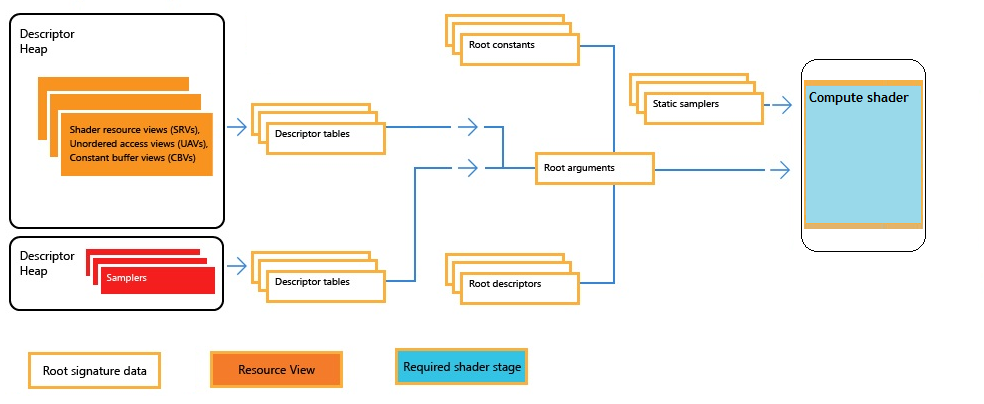
\includegraphics[scale=0.40, keepaspectratio]{img/compute-pipeline.png}
    \caption{El siguiente diagrama ilustra el cauce gráfico Direct3D 12 y su estado.}
    \label{figura:khronos}
\end{figure}

No hay unidades de funciones fijas en esta tubería, sin embargo, la memoria del heap de descriptores muestreos y muestreadores
estáticos todavía están disponibles en el cómputo.

\section{OpenGL} 
\label{sec:OpenGL}

OpenGL es una interfaz de programación que abstrae al desarrollador del hardware o GPU utilizada en su desarrollo.
OpenGL está pensado como una librería de gráficos para desarrolladores de videojuegos o simuladores de entornos virtuales. 

\vspace{1mm} %5mm vertical space

La librería viene con una serie de funciones que aprovechan las características de las especificaciones del estándar.
El hardware debe proveer al usuario de un driver que cumpla con las especificaciones de OpenGL para poder aprovechar
sus características de cómputo gráfico. 

\vspace{1mm} %5mm vertical space

OpenGL funciona en sistemas operativos Linux y MacOS y también funciona en sistemas operativos Windows al ser una
especificación que debe seguir el fabricante del driver de la tarjeta gráfica y no depender del sistema operativo.

\vspace{1mm} %5mm vertical space

La API OpenGL facilita el desarrollo de aplicaciones multiplataformas pudiendo desplegar el proyecto realizado en
diferentes entornos hardware que cumplan con la especificación del estándar en algunas o en la totalidad de sus
versiones de OpenGL.

\subsection{Introducción a OpenGL} 
\label{subsec:IntroOpenGL}

En las versiones anteriores de OpenGL 3.3, la especificación no daba una flexibilidad a los desarrolladores, era una
especificación más simple donde el driver era el encargado de realizar la mayoría de las tareas de computación
gráfica pero de manera poco eficiente, en las nuevas especificaciones de OpenGL se deja más libertad al desarrollador
pudiendo interferir en el núcleo del cauce de procesamiento gráfico, dando más flexibilidad y aumentando la eficiencia
de las aplicaciones gráficas. Estos dos modelos de programación son lo que se denominan modo inmediato y modo perfilado
del núcleo siendo el segundo el usado en las nuevas especificaciones de la API. En el uso del modo perfilado del núcleo
a partir de OpenGL 3.3, las versiones posteriores únicamente añaden nueva funcionalidad y eficiencia sin cambiar el
modelo de programación por este motivo se ha decidido realizar el proyecto utilizando la versión de OpenGL 3.3.

\vspace{1mm} %5mm vertical space

Es posible utilizar funcionalidades que soporte el fabricante de la tarjeta gráfica fuera de la especificación de OpenGL
como extensiones. Cuando una extensión se hace popular o es realmente útil a la hora de realizar un procesamiento o
técnica gráfica es añadida a la especificación de OpenGL, sin embargo a la hora de la implementación podemos añadir
extensiones y comprobar que en la plataforma donde se va a utilizar la extensión el driver la soporta y en tal caso
utilizarla o si no realizar el algoritmo gráfico a la manera antigua o legacy.

\vspace{1mm} %5mm vertical space

OpenGL está pensada como una máquina de estados, esta máquina de estados es lo que se denomina el contexto de OpenGL.
La máquina de estados está definida como un conjunto de variables que determinan cuál va a ser el comportamiento de OpenGL.
La idea del uso del contexto es cambiar la máquina de estados a través de variables añadiendo opciones y renderizar usando
el contexto actual de la máquina de estados. Muchas de las funciones de OpenGL son utilizadas únicamente para realizar un
cambio en la máquina de estados de la que luego beneficiarse a la hora de realizar la renderización de los objetos.

\vspace{1mm} %5mm vertical space

La especificación de OpenGL debe estar escrita en C, los drivers de los fabricantes de tarjetas gráficas que han seguido
las especificaciones de OpenGL han desarrollado el driver en C y por tanto no cuentan con características de lenguajes
de alto nivel, para solucionar este problema OpenGL cuenta con abstracciones para el uso de objetos a través de estructuras de datos.

\vspace{1mm} %5mm vertical space

Para terminar comentar que un objeto de OpenGL que utilizaremos en el desarrollo del proyecto son un subconjunto de estados
de OpenGL y que representan una entidad como puede ser la ventana de OpenGL donde podemos modificar algunos atributos del
objeto como su tamaño, la cantidad de colores que soporta la ventana o si la ventana es panorámica o no, entre otras
propiedades de la entidad ventana.

\vspace{1mm} %5mm vertical space

Una vez explicado OpenGL en el siguiente apartado se define la estructura dinámica de ejecución de OpenGL dentro de la máquina
de estados y el paso de una estructura de datos de una geometría en 3D a valores entendibles por la pantalla en la fase final
de renderizado del objeto pixelado.

\subsection{El cáuce gráfico de OpenGL} 
\label{subsec:CauceOpenGL}

El cauce gráfico de OpenGL se inicia cuando se quiere renderizar algún objeto 3D por pantalla esta transformación de renderizado,
pasar de un objeto geométrico 3D a un conjunto de valores RGB como parte final del renderizado se realiza a través de un pipeline
definido por etapas.

\vspace{1mm} %5mm vertical space

El cauce gráfico está dividido en dos grandes etapas divididas en etapas más especializadas. La primera etapa se pasa de un objeto
o geometría en un espacio de coordenadas en 3D a un objeto plano 2D. En la segunda etapa del cauce se rellenan los píxeles de la
pantalla con los colores de la parte final de los objetos ya en 2D de la etapas previas del cauce.

\vspace{1mm} %5mm vertical space

Cada etapa del cauce cuenta con una entrada de datos y una salida procesada que será la entrada de la siguiente etapa del cauce
hasta obtener un valor final de renderizado y rellenar los píxeles de pantalla con un valor RGB.

\begin{figure}[H]
    \centering
    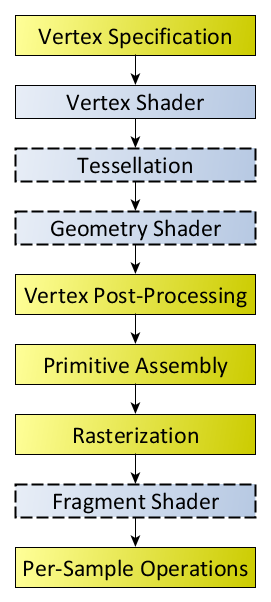
\includegraphics[scale=0.40, keepaspectratio]{img/RenderingPipeline.png}
    \caption{Imagen del cauce gráfico de OpenGL en sus diferentes etapas del cauce gráfico hasta la renderización.}
    \label{figura:khronos}
\end{figure}

Cada una de las etapas del cauce está especializada en una tarea (tienen una función específica), de esta manera es fácil
paralelizar la entrada de datos con operaciones SIMD (Single Instruction Multiple Data) y utilizar la arquitectura masivamente
paralela de una GPU. Cada etapa del cauce realizará el procesamiento paralelo con los datos de entrada, dependiendo de la
flexibilidad de la etapa se podrán realizar programas implementando algoritmos gráficos definidos por el desarrollador,
estas etapas más flexibles del cauce son las etapas programables mientras que otras etapas son únicamente etapas configurables.


\begin{itemize}
  \item Los programas que se desarrollan y ejecutarán en la GPU con los datos de entrada del cauce anterior se denominan programas
  de shaders y existen en todas las librerías de gráficos.
  
  \item Las etapas del cauce de la especificación de OpenGL están definidas como etapas que se denominan primitivas hasta las etapas
  finales de renderizado igual que ocurre en otras librerías gráficas.
\end{itemize}

En la primera etapa la etapa de especificación de vértices, se define una lista ordenada de límites o primitivas que serán el conjunto
total de los datos. Estos datos son representados en forma de atributos, como subconjunto de datos, cada subconjunto de datos
representa un vértice de la primitiva.

\vspace{1mm} %5mm vertical space

El conjunto total de atributos o vértices se denomina VAO (Vertex Array Object). Un ejemplo de definición de primitivas o array de
vértices puede tener un total de dieciocho valores, si definimos el valor de medida de un atributo en tres unidades, OpenGL
interpretará que tiene seis vértices dentro buffer de vértices representado por tres datos que en las siguientes etapas del
cauce se definirá como un vector de tres dimensiones. El valor del conjunto de atributos es arbitrario en esta etapa, es en las
siguientes etapas de vértices donde esta definición de atributo tiene un sentido espacial.

\vspace{1mm} %5mm vertical space

Una vez terminada la especificación del buffer de vértices en la CPU se realiza el renderizado de vértices con la llamada de
función de pintar primitivas de OpenGL glDrawArrays y comienzan a procesarse las diferentes etapas del cauce dentro de la GPU.

\vspace{1mm} %5mm vertical space

La siguiente etapa importante del cauce ya dentro del procesamiento de la GPU es la etapa de shaders de vértices, una etapa
programable del cauce. 

\begin{itemize}
  \item La etapa realiza un procesamiento básico sobre cada vértice de forma individual y define un valor de salida de vértice
  definido por el procesamiento del programa de shaders realizado por el desarrollador. 
  
  \item Las salidas están definidas por el desarrollador pero siempre espera una salida para cada atributo de entrada, mapeado 1:1
  la entrada y salida de vértices, esto se debe a que no pueden compartirse estados entre vértices por propósitos de rendimiento
  en el paralelismo del procesamiento de los mismos.
\end{itemize}

La etapa de shader de geometrías sigue trabajando a nivel de primitivas, devolviendo a su salida un valor nulo o un mayor número de
salidas de primitivas, 0:N, esta etapa también es una etapa programable del cauce.

\begin{itemize}
  \item Permite al desarrollador generar un mayor número de primitivas o eliminar algunas de ellas, de esta manera se puede conseguir
  una mejor definición de las primitivas homogéneas o similares en el procesamiento de la GPU y conseguir un mejor rendimiento en la
  definición de la geometría.
  
  \item Puede cambiar la definición de la primitiva inicial de un punto una línea o triángulo a cada una de ellas, respectivamente.
\end{itemize}

Una vez finalizada la etapa de geometrías empiezan las siguientes etapas del cauce gráfico relacionadas con el post procesamiento
de los vértices o primitivas.

\begin{itemize}
  \item La etapa de clipping o recorte, se encarga de separar las primitivas en un subconjunto de primitivas que están dentro de la
  ventana y de la perspectiva eliminando las primitivas interiores del volumen que no pueden ser vistas en el renderizado final,
  teniendo como referencia la matriz de vista del modelo proyectado generalmente por una cámara.
  
  \item En la etapa de ensamblado de las primitivas, dada una entrada de vértices se realiza la serialización de las primitivas
  definidas por el usuario en las etapas anteriores, si se definieron 12 vértices como un array de triángulos en esta etapa se
  generarán 10 triángulos en base a la definición previa de la primitiva básica y el orden de definición de los vértices de la
  primitiva, ya sea por orden de entrada o por el orden definido en un array de índices de la primitiva.

  \item Existe una última operación en el post procesamiento de vértices, etapa de culling, esta etapa se encarga de descartar las
  primitivas finales que no estén dentro de la ventana proyectada por la cámara, evitando el cómputo innecesario de primitivas en
  el renderizado final de los fragmentos.

  \item En la etapa de rasterización las primitivas son rasterizadas en el orden que entran por esta etapa dividiendo las primitivas
  en una estructura de datos denominados fragmentos.
\end{itemize}

Un fragmento es un conjunto de estados que se utiliza para calcular los datos finales de un pixel o de una muestra si se tiene
habilitado el MSAA (Multiple Sampling Anti Aliasing) en el framebuffer de salida. El estado del fragmento incluye su posición
en el espacio de la pantalla y una lista de datos arbitrarios que se obtuvieron del vértice o en la etapa de shaders de geometrías
después de pasar por la etapa de rasterización.

\begin{itemize}
  \item En la etapa de shaders de fragmentos se realiza un procesamiento sobre los fragmentos. La salida de la etapa de fragmentos es
  un valor de color dado a cada fragmento, incluyendo un valor de profundidad del fragmento previo.  En esta etapa tenemos control
  del valor de salida tanto de profundidad como de color final del fragmento. 
  
  \item La etapa de fragmentos es una etapa programable y es un etapa opcional, si no se define un programa de shaders para la etapa
  de fragmentos el valor de renderización final es el buffer de profundidad, calculado por el posicionamiento de las primitivas de
  las etapas anteriores.

  \item Las etapas de fragmentos realizan una serie de operaciones por pixel o muestra. Estas etapas están definidas por un conjunto
  de tests que son aplicados a los fragmentos, si el test falla el fragmento se descarta, no se renderiza en pantalla, algunos de
  estos tests más importantes son el test de profundidad para no pintar objetos superpuestos, haciendo uso del valor de profundidad
  de los fragmentos.
\end{itemize}

La última parte del cauce realiza una serie de test sobre los fragmentos decidiendo si el fragmento se renderiza o no por pantalla en
su posterior valor a pixel de pantalla.

\begin{itemize}
  \item  La etapa de transparencia de color realiza la operaciones de test para cada color de fragmento, se realizan una serie de
  operaciones lógicas entre el fragmento y el framebuffer de colores permitiendo el paso de color entre objetos y poder renderizar
  materiales que puedan ser transparentes.
\end{itemize}

Por último el fragmento es escrito en el framebuffer de salida que está estructurado por los canales de color y profundidad y mostrando
finalmente la renderización final al usuario por pantalla.

\subsection{Sistema de coordenadas en OpenGL} 
\label{subsec:SysOpenGL}

Por convención, OpenGL es un sistema dextrógiro. Lo que esto básicamente dice es que el eje x positivo está a su derecha, el eje y
positivo está hacia arriba y el eje z positivo está hacia atrás. Pensando en la pantalla como el centro de los 3 ejes y el eje z positivo
que atraviesa la pantalla hacia el usuario del ordenador. Los ejes se dibujan de la siguiente manera:

\begin{figure}[H]
    \centering
    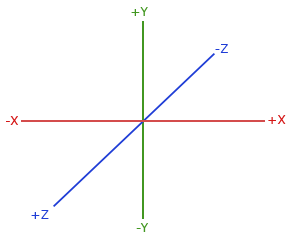
\includegraphics[scale=0.40, keepaspectratio]{img/coordinate_systems_right_handed.png}
    \caption{Sistema de coordenadas en OpenGL}
    \label{figura:khronos}
\end{figure}

Para entender por qué se llama dextrógiro, se debe hacer lo siguiente:

\begin{itemize}
  \item Estirar el brazo derecho a lo largo del eje y positivo con la mano hacia arriba.
  \item Dejar el pulgar apuntando a la derecha.
  \item Dejar que el dedo índice señalar hacia arriba.
  \item Doblar el dedo medio hacia abajo 90 grados.
\end{itemize}

Si se sigue ese procedimiento, el pulgar debe apuntar hacia el eje x positivo, el dedo índice hacia 
el eje y positivo y el dedo medio hacia el eje z positivo. Si se hace esto con el brazo izquierdo,
el eje z está invertido. Esto se conoce como un sistema levógiro y es utilizado comúnmente por DirectX.
Hay que tener en cuenta que en las coordenadas de dispositivo normalizadas, OpenGL en realidad usa un
sistema zurdo, la matriz de proyección cambia la mano al modo dextrógiro.

\section{Entorno y herramientas} 
\label{sec:Entorno}

A continuación se nombran las implementaciones abiertas de la librería de OpenGL, entorno y herramientas 
utilizadas para el proyecto, en este caso el uso de glfw3 con glad y la ayuda de la librería de matemática
para gráficos compatible con la especificación OpenGL, GLM (OpenGL Mathematics Library).

\subsection{Glad} 
\label{subsec:Glad}

Esta es una herramienta para generar cargadores de funciones OpenGL. Selecciona el lenguaje, las versiones
de OpenGL / OpenGL ES, los perfiles principales o compatibles, y los genera en un fichero de cabecera.

\vspace{1mm} %5mm vertical space

La herramienta genera el fichero de cabecera con las declaraciones de la interfaz de las funciones GL y
las estructuras de datos para la versión de GL que se elija, y genera un pequeño archivo fuente C que
resuelve todas las funciones en tiempo de ejecución para ayudar al compilador en la definición de
símbolos y tipos de datos de las funciones de la librería de OpenGL antes de enlazar con la librería
gráfica binaria instalada en el sistema operativo y generar el fichero binario de la aplicación gráfica
definida por el desarrollador.

\vspace{1mm} %5mm vertical space

A la hora de definir los includes en el programa con la definición de las funciones de la librería de
OpenGL se debe cargar primero el fichero de cabecera generado por la herramienta GLAD para resolver de
manera correcta las estructuras de datos y las definiciones de funciones de OpenGL en el entorno de
desarrollo.

\subsection{GLFW} 
\label{subsec:GLFW}

GLFW es una biblioteca multiplataforma de código abierto para el desarrollo de OpenGL, OpenGL ES y Vulkan,
en plataformas de escritorio. Proporciona una API simple para crear ventanas, contextos y superficies
gráficas y recibir entradas o eventos de los periféricos, está escrito en C y es compatible con los sistemas
operativos Windows, macOS y Linux.

\vspace{1mm} %5mm vertical space

Las ventajas de usar la librería GLFW con la implementación de algunos de los estándares gráficos son
las siguientes:

\begin{itemize}
  \item Se puede obtener una ventana y un contexto de OpenGL utilizando dos llamadas a la
  función de la API.

  \item Soporta OpenGL OpenGL ES, Vulkan y algunas de las opciones extendidas de las
  especificaciones.

  \item Soporta el uso de múltiples ventanas y múltiples monitores con alta densidad de
  píxeles o alta resolución (high-DPI).

  \item Tiene soporte para entradas de teclado ratón eventos de ventana y gamepad haciendo
  uso de polling sobre los dispositivos o utilizando manejadores de eventos, haciendo fácil
  el uso de periféricos dentro de las aplicaciones.

  \item La librería viene con tutoriales con código de ejemplo y documentación de las
  funciones de la API.

  \item Tiene acceso a objetos nativos en tiempo de compilación para características específicas
  de ciertas plataformas.

  \item Existe una comunidad que da soporte y mantiene la librería actualizada en diferentes
  lenguajes de programación.

\end{itemize}

La herramienta GLFW es la encargada de generar la entidad o ventana del contexto de OpenGL.

\subsection{OpenGL Mathematics Library GLM} 
\label{subsec:GLM}

OpenGL Mathematics (GLM) es una biblioteca matemática desarrollada en C++ solo para software
de gráficos basada en las especificaciones de OpenGL de su lenguaje de shaders Shading Language (GLSL).
GLM proporciona clases y funciones diseñadas e implementadas con las mismas convenciones de nombres
y funcionalidades que GLSL para que cualquiera que conozca GLSL, pueda usar la librería GLM también
en la CPU a través de lenguajes de programación cómo C++.

\vspace{1mm} %5mm vertical space

Este proyecto no se limita a las funciones GLSL. Un sistema de extensión, basado en las convenciones
de extensión GLSL, proporciona capacidades extendidas: transformaciones matriciales, cuaterniones,
empaquetamiento de datos, números aleatorios, ruido, etc. Por lo que muchas operaciones de lenguaje
de shaders que se ejecutan dentro de la GPU pueden ser portadas también a la CPU, utilizando esta librería.

\vspace{1mm} %5mm vertical space

Esta biblioteca funciona perfectamente con OpenGL pero también garantiza la interoperabilidad con otras
bibliotecas de terceros y SDK o librerías externas que no tengan que ver con OpenGL. Es un buen candidato
para la representación de software (trazado de rayos / rasterización), procesamiento de imágenes,
simulaciones físicas y cualquier contexto de desarrollo que requiera una biblioteca matemática gráfica.

\vspace{1mm} %5mm vertical space

GLM está escrito en C++ 98 pero puede aprovechar C++ 11 cuando es compatible con el compilador. Es una
biblioteca independiente de la plataforma y oficialmente admite la mayoría de los compiladores de C++
más utilizados en la industria.

\begin{figure}[H]
    \centering
    
\includegraphics[scale=0.80, keepaspectratio]{img/logo_glm.png}
    \caption{Logotipo de la librería matemática compatible con las especificaciones del lenguaje GLSL.}
    \label{figura:logo_glm}
\end{figure}

\subsection{OpenGL Utility Libraries GLUT} 
\label{subsec:GLUT}


La librería glut es un conjunto de herramientas externas que trabajan con el core de OpenGL,
su finalidad es servir de interfaz con diferentes dispositivos de entrada y salida heterogéneos,
utilizados en el campo de realidad virtual.

\vspace{1mm} %5mm vertical space

Ahora se hablará de algunos de los motores gráficos que utilizan todas o algunas de estas
tecnologías para que el usuario pueda realizar aplicaciones gráficas de forma sencilla evitando
el uso de las librerías gráficas y paradigmas de programación vistos de bajo nivel.

\section{Motores Gráficos} 
\label{sec:Motores}

En este apartado realizaremos una introducción de tres de los motores gráficos más utilizados
en la actualidad; Unreal, Unity y Blender. Para realizar la simulación utilizaremos blender y
realizaremos una mayor profundidad en el uso de este motor gráfico en la fase final de resultados.

\subsection{Unreal} 
\label{subsec:Unreal}

Unreal es un motor gráfico desarrollado por la compañía Epic Games, sus primeras versiones fechan del año
1998, el desarrollo del motor está realizado en C++ y sus versiones son Open Source. Su página web cuenta
con una documentación de todas las funcionalidades del motor además de tutoriales. Unreal cuenta con una
comunidad activa que realizan aportaciones al desarrollo y diseño del motor además de preguntas a problemas
que puedan tener otros usuarios. El motor está pensado como un conjunto de módulos y herramientas para
facilitar la creación de contenido gráfico.

\vspace{1mm} %5mm vertical space

El desarrollo de las aplicaciones gráficas en Unreal puede desplegarse en multiplataforma, desde sistemas
operativos Windows hasta máquinas embebidas de realidad virtual de Valve o Samsung, teléfonos móviles o
consolas de manera gratuita. Unreal cobra por el uso de la plataforma el cinco por ciento de las aplicaciones que
superen una cuota de mercado mayor de 3000 dólares.

\vspace{1mm} %5mm vertical space

Entre las características principales del motor Unreal cuenta con un módulo de renderizado de gráficos, este
módulo se encarga de la simulación de luces, generación de sombras carga de materiales y texturas, efectos
de partículas o post procesado. Es decir la parte principal de renderización y visualización de las geometrías.

\vspace{1mm} %5mm vertical space

Cuenta con un módulo para el desarrollo de interfaces de usuario Unreal Motion Graphics User Interfaces UMG.
La interfaz de usuario hace uso de Widgets para la captura de eventos de usuario a través de botones barras
de progreso, menús etc. Esta interfaz interactiva ayuda al desarrollador a crear contenido de manera muy
sencilla y realizar cierta lógica de animación o jugabilidad sin tener conocimientos sobre programación.

\vspace{1mm} %5mm vertical space

Uno de los principales módulos de Unreal y más conocido con los Blueprint Visual Scripting. Este módulo
está diseñado como un diagrama de flujo o una máquina de estados presentado como un visualización en
bloques con un flujo de ejecución.

\begin{figure}[H]
    \centering
    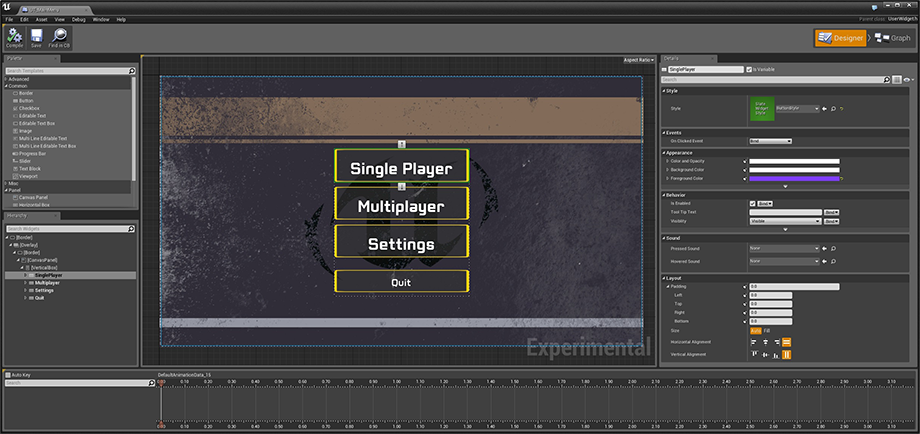
\includegraphics[scale=0.30, keepaspectratio]{img/menu_unreal.png}
    \caption{Uso de flujo de programa utilizando la interfaz blue visual scripting}
    \label{figura:menu_unreal}
\end{figure}

La idea es utilizar esta interfaz de visualización para usuarios con poca experiencia en programación
y poder generar comportamientos animaciones u objetos gráficos con materiales de manera rápida y
sencilla que solo podrían ser accesibles para desarrolladores o personas con conceptos de programación.

\begin{figure}[H]
    \centering
    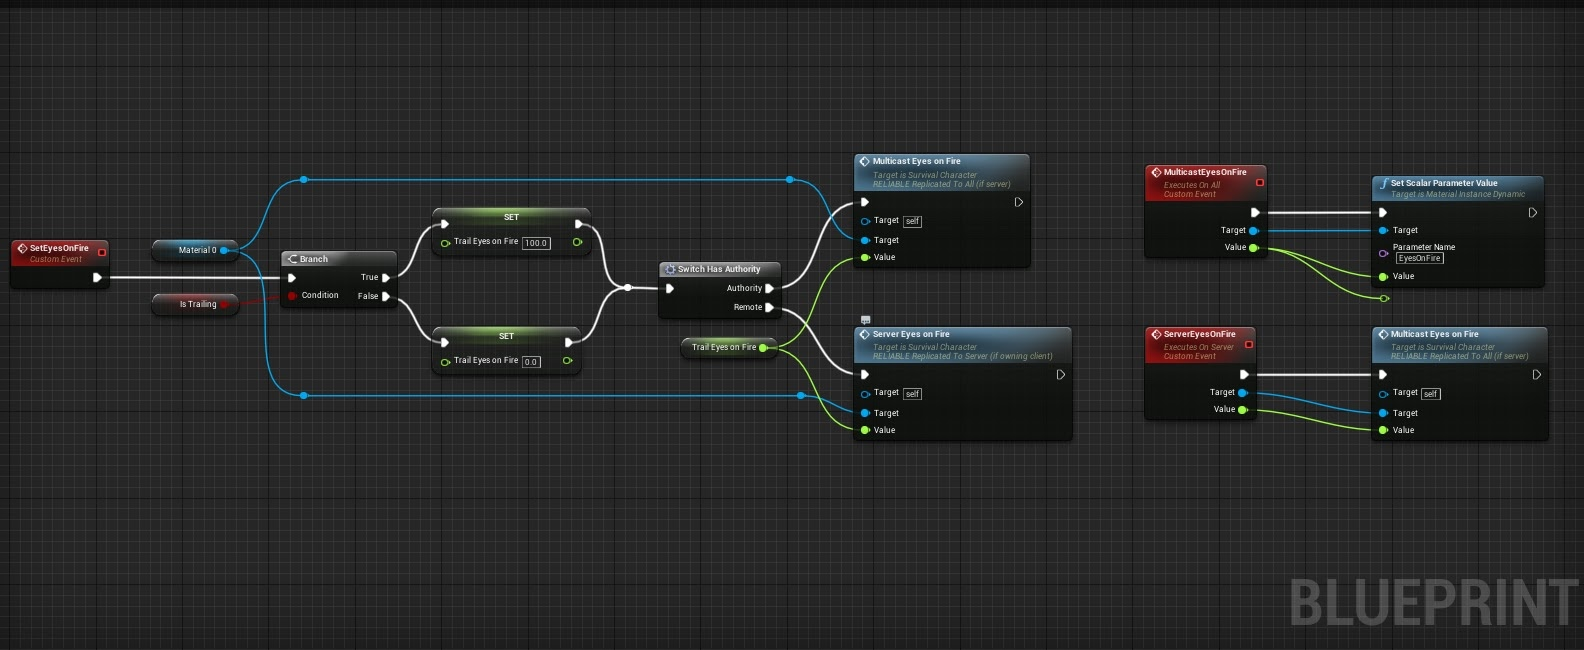
\includegraphics[scale=0.15, keepaspectratio]{img/option1_unreal.jpg}
    \caption{Uso de flujo de programa utilizando la interfaz blue visual scripting}
    \label{figura:option1_unreal}
\end{figure}

Hace uso de una API para realizar un flujo de ejecución y lógica de las aplicaciones, en lenguajes de
programación C++ y Luna. La API de C++ es clara y sencilla de utilizar aunque se deben tener conocimientos
previos de programación en este lenguaje para poder utilizar esta API. Esta dificultad puede ser resuelta
con el uso del módulo de  Blueprint Visual Scripting que utiliza por debajo la misma API del motor para
generar la lógica o flujo de ejecución de las animaciones.

\vspace{1mm} %5mm vertical space

Unreal trata de ser un motor gráfico genérico e innovador para la realización de contenido gráfico de
simulaciones virtuales o animación cinematográfica. El uso de lenguaje C++ como el uso del editor o
algunos módulos del motor requieren de un conocimiento previo del funcionamiento de físicas, geometrías
o materiales en entornos gráficos, esto dificulta la curva de aprendizaje de la plataforma.

\vspace{1mm} %5mm vertical space

Uno de los principales puntos fuertes de Unreal es su buen uso de los recursos, con una buena gestión
de la memoria y del cauce gráfico en el renderizado de los objetos o las físicas dentro de la plataforma
a pesar de su complejidad. 

\vspace{1mm} %5mm vertical space

El competidor directo de Unreal en el desarrollo de videojuegos multiplataforma en la actualidad es el
motor gráfico Unity 3D.

\subsection{Unity 3D} 
\label{subsec:Unity3D}

Unity es un motor gráfico pensado para el desarrollo de aplicaciones gráficas multiplataforma en tiempo
real. Sus principales usos son el desarrollo de videojuegos y la creación cinematográfica de animación.
La plataforma de Unity contiene partes gratuitas Open Source y otras privativas que pueden ser explotadas
con la adquisición de licencias con un coste adicional.

\vspace{1mm} %5mm vertical space

Unity cuenta con una interfaz potente para importar archivos externos heterogéneos y su uso dentro del
espacio de trabajo de un proyecto creado en Unity.  La importación de archivos cuenta con importación
de ficheros de audio y sonido, renderizados 3D realizados en otras plataformas de diseño gráfico como
autocad o malla o importación de fuentes de lenguaje e idiomas.

\begin{figure}[H]
    \centering
    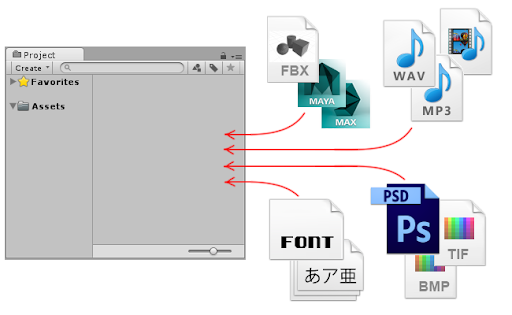
\includegraphics[scale=0.60, keepaspectratio]{img/unity_assets.png}
    \caption{Visualización del uso de la librería Assets para importación de archivos en Unity}
    \label{figura:unity_assets}
\end{figure}

Unity también cuenta con primitivas pre definidas para objetos geométricos básicos como esferas cubos
ellipses o planos, parecido al utilizado en el proyecto, haciendo uso de funciones matemáticas parametrizadas
para generar las primitivas, tamaños o formas de las superficies.

\vspace{1mm} %5mm vertical space

El foco de atención principal del usuario en Unity se hace a través de la ventana principal, dentro de
la ventana principal se pueden cargar en diferentes pasos el desarrollo de las aplicaciones gráficas,
es decir ventanas con funciones específicas del motor se cargan dentro de la ventana principal. 

\vspace{1mm} %5mm vertical space

En la ventana de proyecto se pueden manejar los materiales geometrías o archivos externos cargados con la
interfaz Assets. La ventana de proyecto se puede gestionar en un panel adicional donde está contenida la
estructura de directorios del proyecto y los ficheros importados. En la ventana de proyecto se puede cargar
una sub ventana en la que se pueden ver los tipos de archivos cargados en la estructura de directorios,
geometrías, texturas, programas de shaders de materiales, ficheros de audio etc.

\vspace{1mm} %5mm vertical space

La vista de escena en la ventana principal, muestra al usuario una visión interactiva del mundo creado con
Unity en la que se podrán editar las luces de la escena posición de los objetos y las cámaras. Esta vista
es fácil de manejar para los usuarios que utilizan por primera vez el motor de Unity y para hacerse una
idea del trabajo con el entorno de desarrollo.

\vspace{1mm} %5mm vertical space

En la vista de juego dentro de la ventana principal se podrá ver el resultado final de la aplicación gráfica
creada con Unity en la que deberemos ver la perspectiva desde cámaras de la escena y el renderizado en tiempo
real de la aplicación.

\vspace{1mm} %5mm vertical space

En esta vista los cambios realizados de forma interactiva son temporales. Como la bajada de la resolución para
emular el uso de dispositivos antiguos o con menor poder computacional. La ventana además avisa al usuario si
no existen cámaras en la escena para advertir de que no hay ninguna vista que pueda ser utilizada por el módulo
de renderizado.

\vspace{1mm} %5mm vertical space

En la ventana de jerarquías podemos ver las dependencias que existen entre los objetos de la escena, algunos de
estos objetos pueden ser geometrías cargadas con la interfaz Asset o componentes del motor como luces o cámaras. 

\vspace{1mm} %5mm vertical space

La ventana de jerarquías nos da una visión del árbol de transformadas de Unity y de las dependencias de los
objetos dentro de la escena de manera global. En esta vista se pueden también crear las dependencias entre
los objetos creando nodos hijos de otro objetos y generar partes del árbol de jerarquía de la escena. Aunque
su uso principal es la visualización del árbol de jerarquía, en escenas de juego más complejas.

\begin{figure}[H]
    \centering
    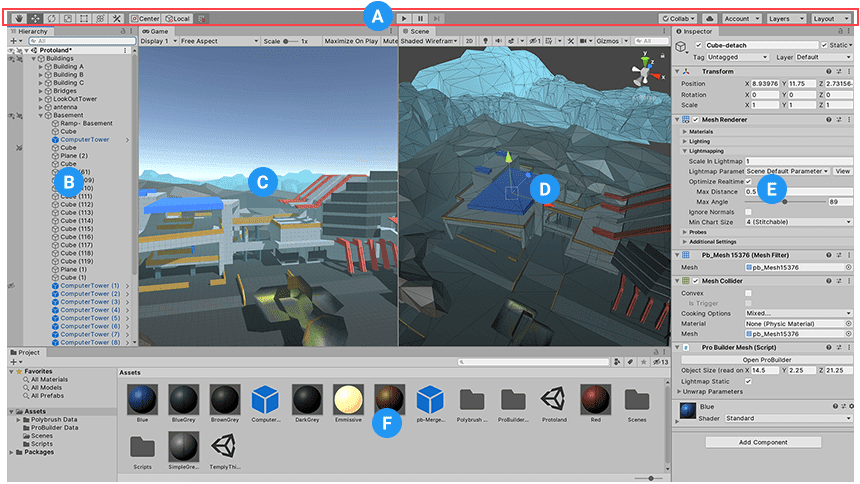
\includegraphics[scale=0.30, keepaspectratio]{img/editor_unity.png}
    \caption{Uso de ventanas en Unity}
    \label{figura:editor_unity}
\end{figure}

El uso de programación también es algo a tener en cuenta dentro de Unity. Muchas aplicaciones necesitan el uso
de de programas para responder a eventos de usuario en el momento que sea necesario, en los scripts es posible
realizar efectos gráficos control de físicas, comportamiento de los objetos o creación de un sistem de inteligencia
artificial personalizado para los objetos de juego. El uso de programación en Unity se realiza a través de la
API de Unity en C\#.

\begin{figure}[H]
    \centering
    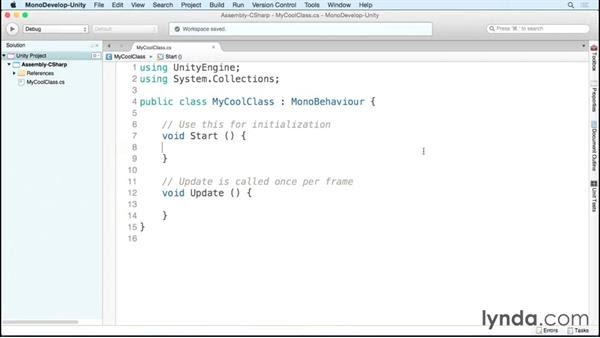
\includegraphics[scale=0.40, keepaspectratio]{img/APIUnity.jpg}
    \caption{Ejemplo de uso de lenguaje de scripting en Unity 3D de componentes}
    \label{figura:APIUnity}
\end{figure}

Unity es un motor con una curva de aprendizaje sencilla en el uso del editor, los conceptos del motor o uso de un
lenguaje de programación de componentes sencillo en C\#. El usuario puede ser capaz de realizar un prototipo de
juego o aplicación virtual de forma rápida. Con el uso del módulo Asset es fácil insertar contenidos de terceros
dentro del motor aunque puede que este contenido se quede corto cuando queremos realizar mundos algo más complejos. 

\vspace{1mm} %5mm vertical space

Los mayores problemas que podemos encontrar en Unity son la mala gestión de los recursos. Al estar implementados
algunos módulos en .Net es posible tener problemas de rendimiento en la gestión de la memoria con el recolector de basura. 

\vspace{1mm} %5mm vertical space

También se encuentran restricciones al no ser un motor completamente Open Source como Unreal, si se quiere realizar
alguna funcionalidad específica que no soporte el motor no se puede añadir.

\vspace{1mm} %5mm vertical space

La inestabilidad entre versiones intermedias también es un problema en Unity ya que en la realización de parches suelen
meterse regresiones y bugs nuevos dentro de la plataforma.

\subsection{Blender} 
\label{subsec:Blender}

Blender es un motor gráfico open source gratuito para la creación de mundos en 3D. El motor blender da soporte completo
para la creación en 3D desde el modelado, la animación, el renderizado, o el seguimiento de objetos. También es posible
realizar animaciones en 2D con blender. El motor blender soporta el cauce completo desde la creación de los objetos 3D
hasta la etapa final de renderizado. Blender se puede utilizar para crear visualizaciones en 3D, como imágenes fijas para
crear texturas, animaciones en 3D, tomas de efectos visuales y edición de video, se adapta bien a desarrollos individuales
y pequeños estudios que se benefician de su proceso unificado de desarrollo y respuesta.

\vspace{1mm} %5mm vertical space

El motor gráfico blender puede realizar desarrollos de aplicaciones gráficas multiplataforma que se ejecuta en sistemas Linux,
macOS y Windows. Blender también tiene requisitos de memoria y procesamiento relativamente pequeños en comparación con otras
plataformas de creación 3D. Su interfaz utiliza OpenGL para proporcionar una experiencia consistente en todo el hardware
y las plataformas compatibles con OpenGL. Tiene una amplia variedad de herramientas que lo hacen adecuado para casi cualquier
tipo de producción de medios, personas y estudios de todo el mundo que lo usan para proyectos de pasatiempos, comerciales y
largometrajes.


\begin{itemize}
  \item Blender es un conjunto de módulos para creación de contenido 3D totalmente integrado, que ofrece una amplia gama de
  herramientas esenciales, que incluyen modelado, renderizado, animación, edición de video, efectos visuales, composición,
  texturizado y muchos tipos de simulaciones.

  \item Es multiplataforma, con una interfaz gráfica de usuario OpenGL que es uniforme en todas las plataformas principales
  (y personalizable con scripts de Python).

  \item Tiene una arquitectura 3D de alta calidad, lo que permite un flujo de trabajo de creación rápido y eficiente.

  \item Cuenta con un apoyo activo de la comunidad, consulte blender.org/community para obtener una lista extensa de sitios.

  \item Tiene un pequeño ejecutable, que es opcionalmente portátil.
\end{itemize}

Blender hace posible realizar una amplia gama de tareas, y puede parecer desalentador cuando se trata de comprender los
conceptos básicos. Sin embargo, con un poco de motivación y el material de aprendizaje adecuado, es posible familiarizarse
con Blender después de algunas horas de práctica.

\begin{figure}[H]
    \centering
    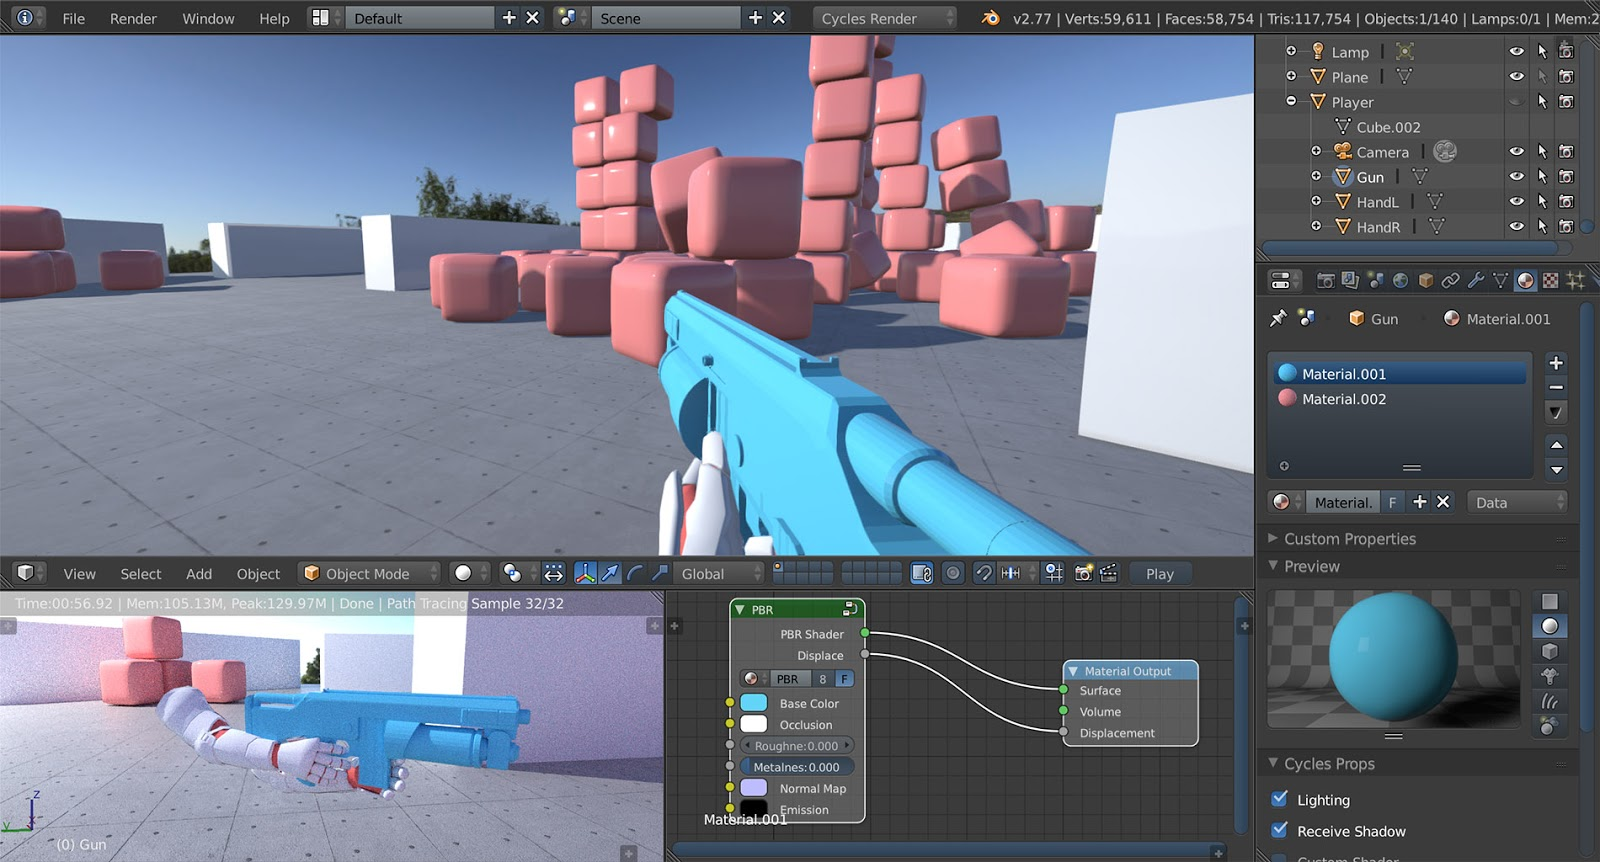
\includegraphics[scale=0.20, keepaspectratio]{img/Blender.jpg}
    \caption{Visualización general de ventanas en blender para la creación de una escena virtual.}
    \label{figura:Blender}
\end{figure}

En la imagen se puede observar: 

\begin{itemize}
  \item La ventana de renderización de la aplicación gráfica

  \item La definición de materiales a través de diagrama de bloques que termina
  convirtiendose en un programa de shader que ejecutará en la tarjeta gráfica.

  \item Ventana de aspecto final del efecto de material con iluminación

  \item El árbol de jerarquía de la escena con los diferentes objetos que la componen.

\end{itemize}

Una vez vistas las tecnologías y los diferentes motores gráficos que se encuentran actualmente en el mercado,
el uso de recursos o la realización de conceptos en los motores gráficos se pasará a ver su aplicación dentro
del desarrollo del motor gráfico del proyecto.


%%%%%%%%%%%%%%%%%%%%%%%%%%%%%%%%%%%%%%%%%%%%%%%%%%%%%%%%%%%%%%%%%%%%%%%%%%%%%%%%
%%%%%%%%%%%%%%%%%%%%%%%%%%%%%%%%%%%%%%%%%%%%%%%%%%%%%%%%%%%%%%%%%%%%%%%%%%%%%%%%
% DISEÑO E IMPLEMENTACIÓN %
%%%%%%%%%%%%%%%%%%%%%%%%%%%%%%%%%%%%%%%%%%%%%%%%%%%%%%%%%%%%%%%%%%%%%%%%%%%%%%%%

\cleardoublepage
\chapter{Arquitectura e implementación del motor gráfico}

El motor está diseñado como una API de alto nivel desarrollada en C++. La interfaz de la API cuenta con un conjunto
de clases públicas para definir abstracciones gráficas y métodos de estas clases para decidir el comportamiento del motor.

\vspace{1mm} %5mm vertical space

La arquitectura está formada por una estructura de datos principal en forma de árbol de nodos, los nodos del árbol
serán los objetos de juego, concepto obtenido del motor gráfico de Unity y Blender.

\vspace{1mm} %5mm vertical space

El diseño de la arquitectura está especificado en un patrón de diseño basado en componentes que formarán la estructura
principal del desarrollo del motor, siguiendo los principios de este diseño, utilizado en los motores Unity o Blender.
Para trabajar el cauce gráfico se utilizará una jerarquía de clases de dibujadores o Drawers que tendrán un comportamiento
de componente especial para saber que objetos de juego son renderizables y deben realizar las operaciones del cauce gráfico.

\vspace{1mm} %5mm vertical space

En la primera parte del desarrollo explicaremos la estructura estática de la arquitectura, la explicación de las clases que
definen las estructuras de datos del motor y las dependencias que existen entre ellas. 

\vspace{1mm} %5mm vertical space

En la segunda parte del desarrollo se explicará de forma detallada la estructura dinámica de la arquitectura explicando paso
a paso las fases de ejecución del motor.

\vspace{1mm} %5mm vertical space

La definición de la estructura estática y dinámica explicarán de forma detallada el funcionamiento del motor gráfico, las
abstracciones gráficas realizadas y la solución al cauce gráfico de OpenGL transparente para el usuario, utilizando técnicas
usadas en otros motores.

\section{Definición estática del motor} 
\label{sec:estatica}

Para definir las clases del motor se empezará por las clases de alto nivel que son utilizadas por el usuario para definir una
escena renderizable en una ventana de OpenGL, según vayan definiéndose las clases de alto nivel se entrará en detalle de las
clases que definen partes de las técnicas gráficas implementadas y su acceso a la interfaz de OpenGL.

La primera clase a explicar es la clase Engine, esta clase almacena la ventana de OpenGL, las instancias de teclado y reloj
para el manejador de eventos de entrada de polling de la interfaz de OpenGL y la escena renderizable dentro de la ventana.
En el constructor recibe como parámetro la escena creada por el usuario para su posterior renderizado en la ventana de OpenGL.
La clase motor cuenta con tres métodos públicos; inicialización actualizado y bucle principal.

\begin{figure}[H]
    \centering
    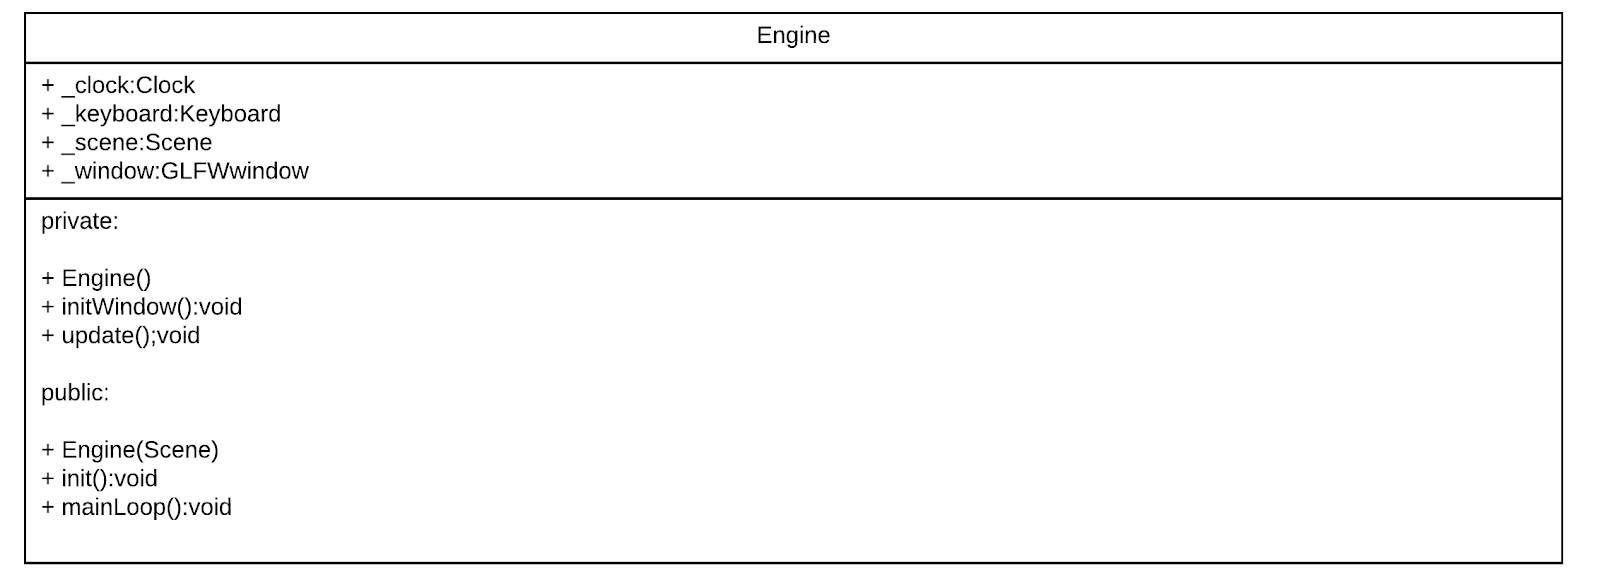
\includegraphics[scale=0.20, keepaspectratio]{img/Engine.png}
    \caption{Diagrama de clases de la clase Engine}
    \label{figura:Blender}
\end{figure}

La clase escena será la responsable de almacenar el objeto raíz que dará acceso a la estructura de datos en árbol del motor y
controlar las diferentes etapas de la arquitectura y su orden de ejecución. Desde fuera el usuario podrá añadir objetos de
juego hijos al objeto de juego raíz para formar el árbol de nodos de la escena. Los objetos de juego hijos a su vez podrán
tener otros objetos de juego hijos que serán accedidos por la escena de forma recursiva en la etapa de ejecución.

\vspace{1mm} %5mm vertical space

La clase escena también contará con la colección de luces para la iluminación de los materiales de los objetos de juego en
la escena y las cámaras, que podrán ser utilizadas para cambiar la perspectiva de vista de la escena desde otros objetos de juego.

\begin{figure}[H]
    \centering
    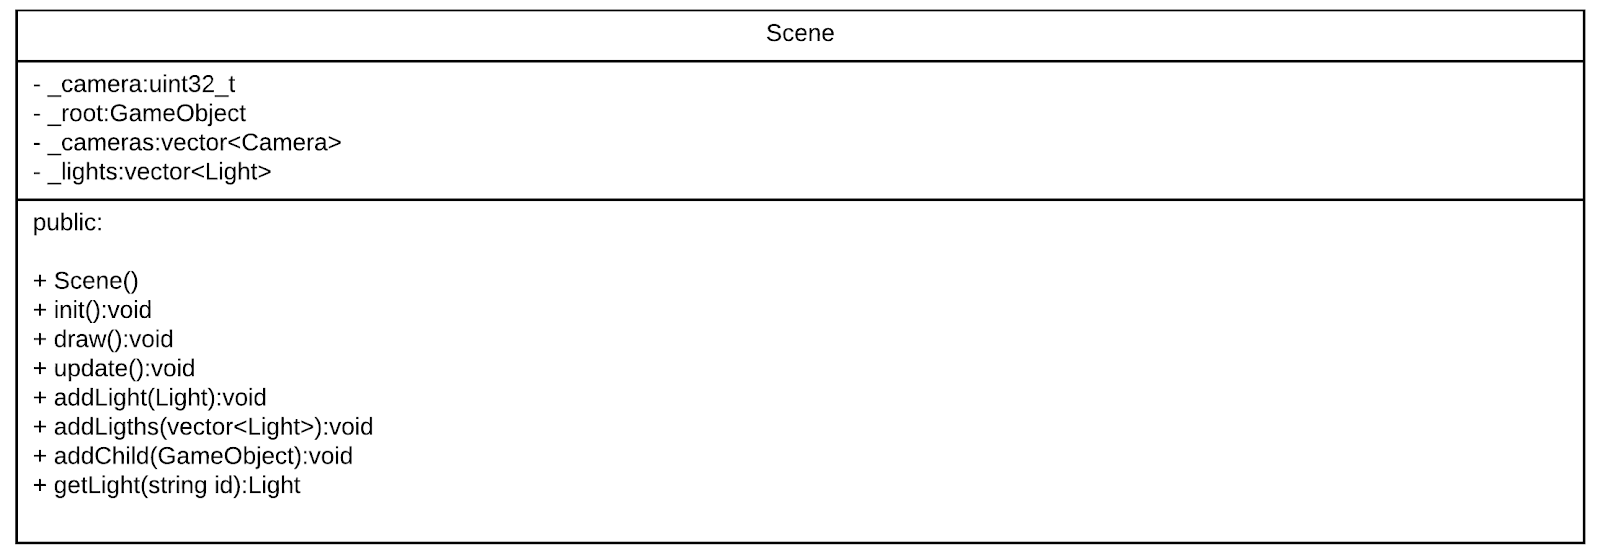
\includegraphics[scale=0.30, keepaspectratio]{img/Scene.png}
    \caption{Diagrama de clases de la clase Scene}
    \label{figura:Blender}
\end{figure}

La clase objetos de juego almacena las componentes que definen el objeto de juego, la colección de objetos de juego hijos para generar
el árbol de escena y el acceso a las luces para iluminar los modelos de los nodos hijos de objetos de juego que sean renderizables.

\vspace{1mm} %5mm vertical space

Todos los objetos de juego cuentan con una componente interna transformada que definen la posición de los nodos de la escena en el
sistema de coordenadas de OpenGL. 

\vspace{1mm} %5mm vertical space

Los objetos cuentan con métodos para realizar operaciones de posicionamiento, escalado o rotación sobre su transformada que serán
accesibles de forma pública para definir el comportamiento en el sistema de coordenadas de OpenGL por el usuario.

\vspace{1mm} %5mm vertical space

Existe un método público para calcular la distancia de un objeto de juego, que recibe como parámetro de entrada el identificador
del objeto de juego del que se quiere saber su distancia dentro del sistema de coordenadas de OpenGL. Este método hará uso de
un método interno de búsqueda que devolverá como resultado la referencia del objeto de juego para realizar el cálculo de distancia
entre ambos objetos.

\vspace{1mm} %5mm vertical space

Para poder realizar técnicas gráficas de transparencia en la fase de renderizado se deben realizar el renderizado de los objetos
que son transparentes con un criterio de ordenación. La clase objetos de juego cuenta con un método interno accesible por la clase
escena para devolver una lista ordenada de objetos. Esta lista realizará el criterio de ordenación por la distancia relativa a la
posición de la cámara principal.

\vspace{1mm} %5mm vertical space

La clase objetos de juego cuenta también métodos para añadir una cámara al objeto de juego y recibir la lista de cámaras de los
nodos hijos. Este método es utilizado por la clase escena para almacenar la colección de cámaras de la escena.

\vspace{1mm} %5mm vertical space

La clase objetos cuenta con los métodos de inicialización, actualización y renderizado que serán posteriormente utilizadas para
llamar a cada una de las componentes en cada una de las etapas de la arquitectura. Estos métodos serán visibles por la clase escena.

\vspace{1mm} %5mm vertical space

Los objetos de juego podrán añadir componentes internas del motor gráfico o componentes externas definidas por el usuario a través
de un método público para este propósito.

\begin{figure}[H]
    \centering
    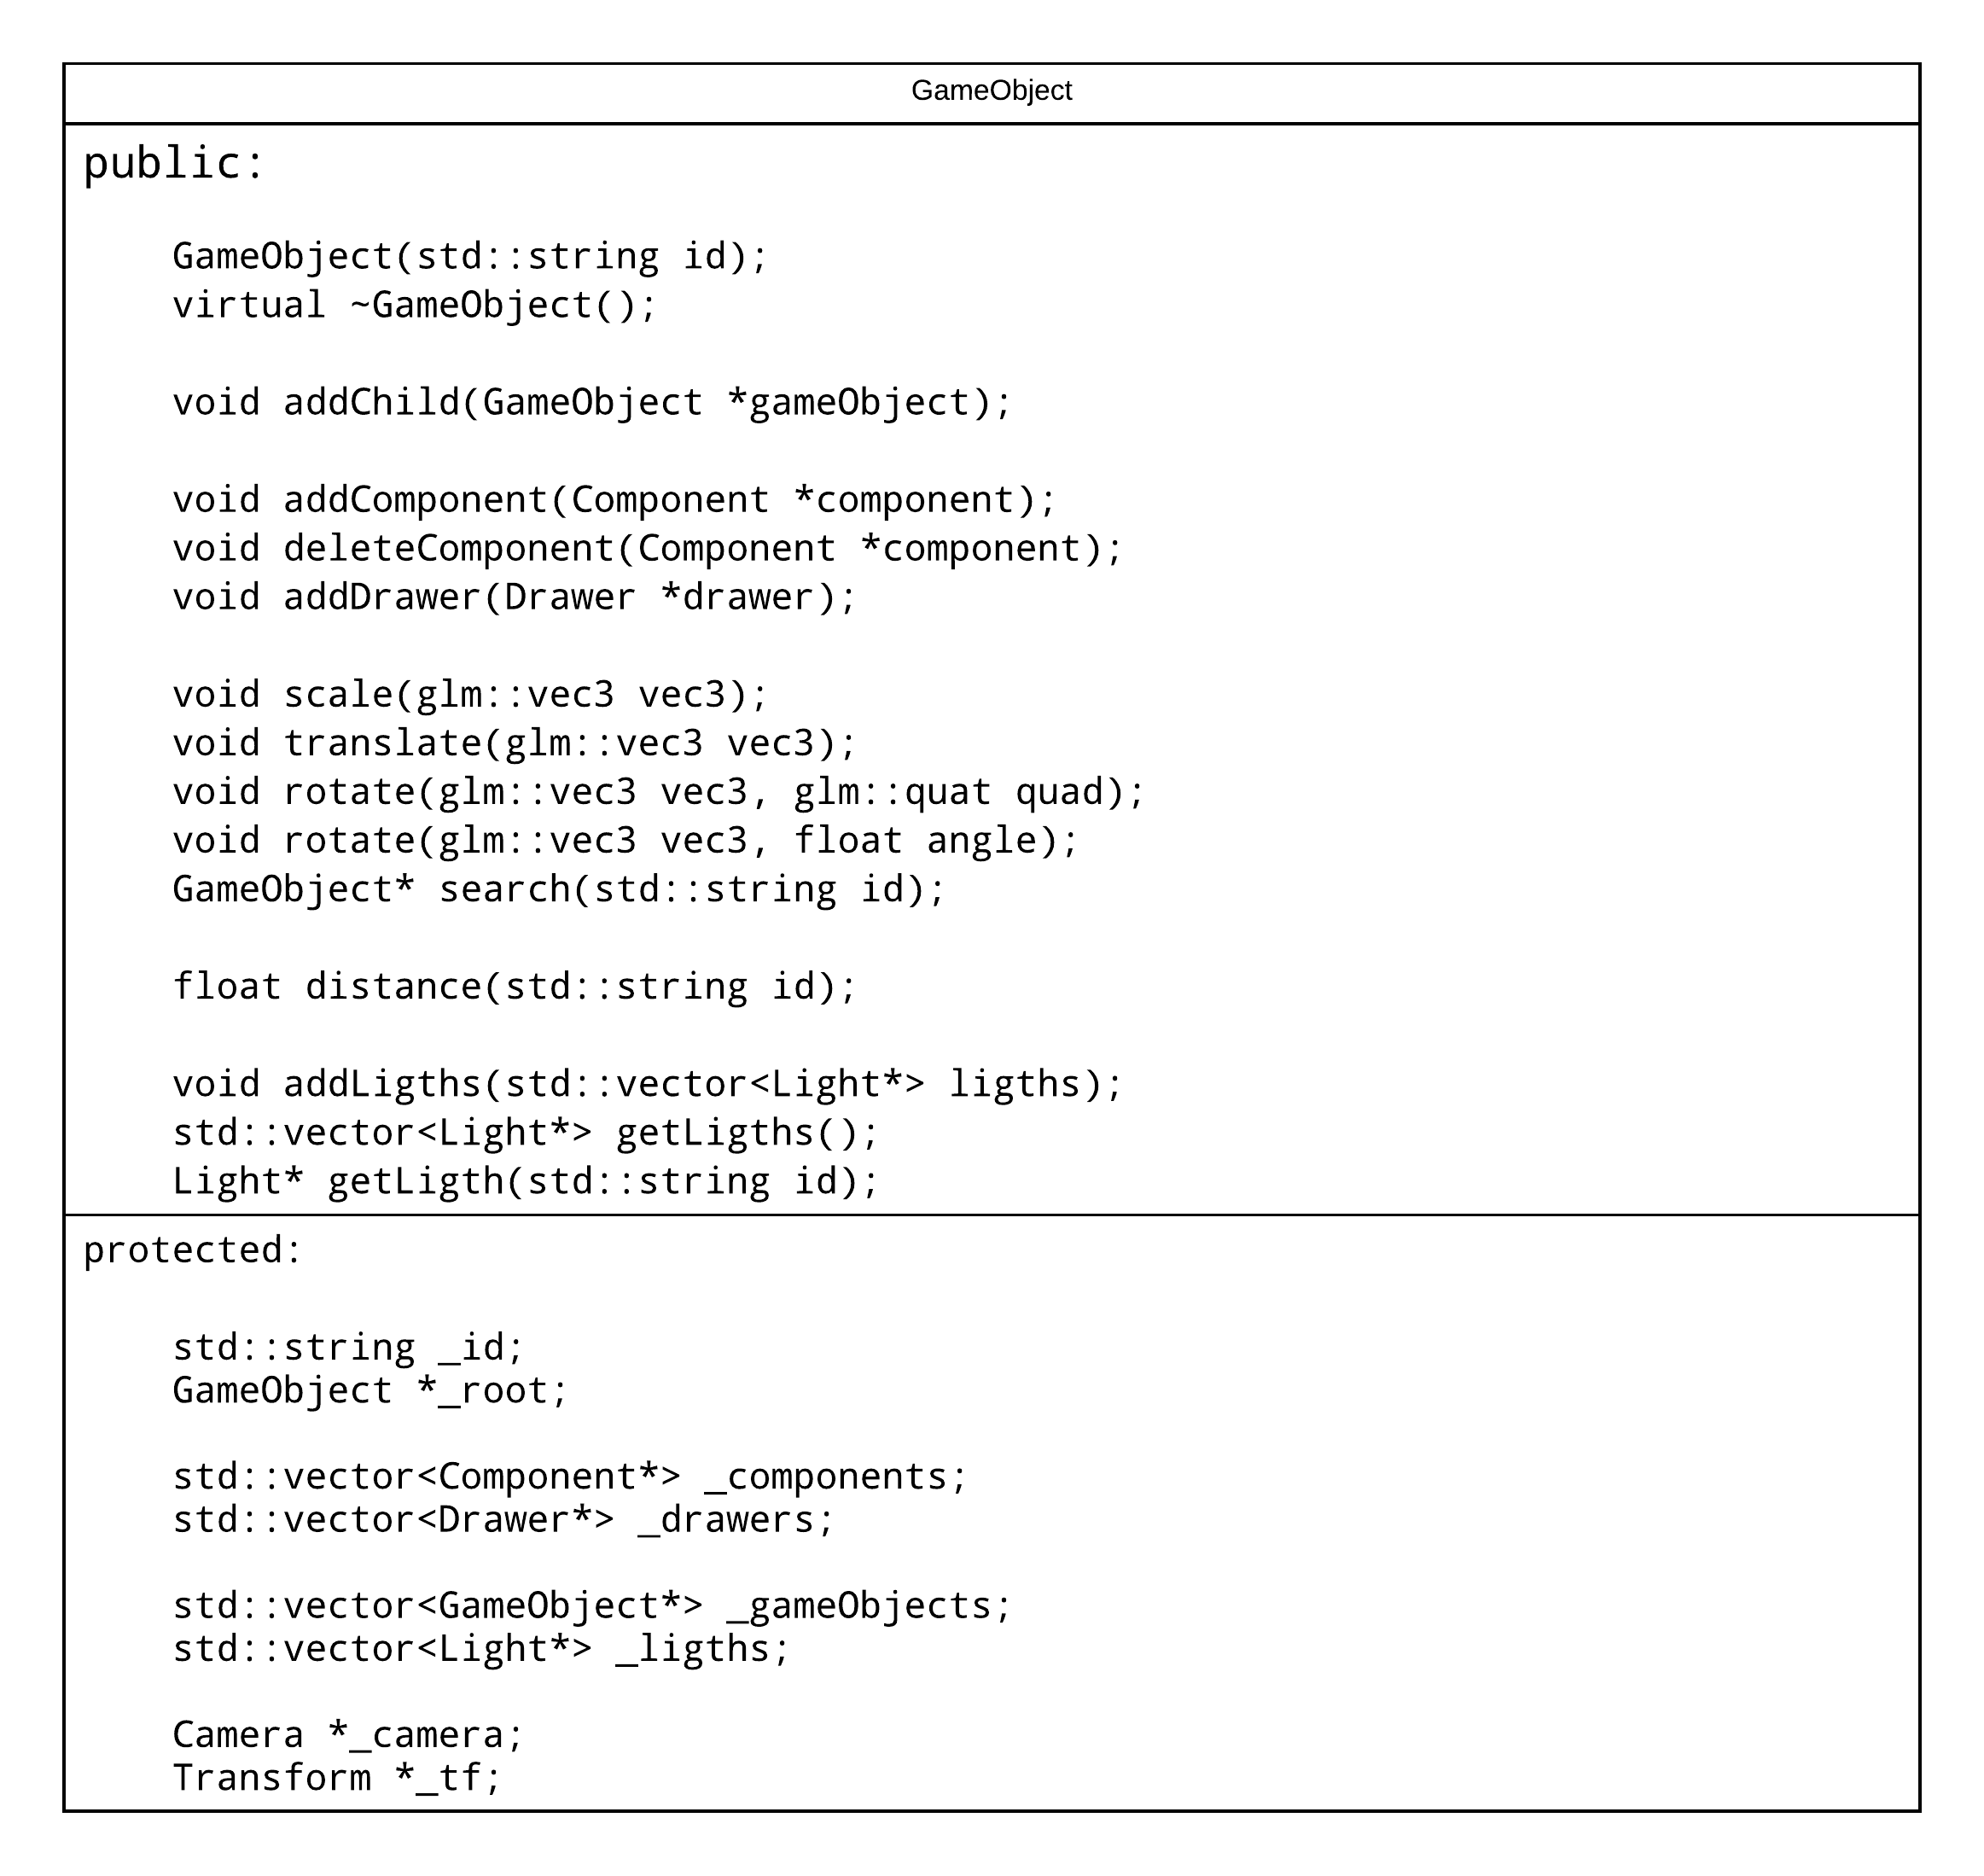
\includegraphics[scale=0.4, keepaspectratio]{img/GameObject.png}
    \caption{Diagrama de clases de la clase GameObject}
    \label{figura:GameObject}
\end{figure}

La clase componentes está definida como una clase virtual que cuenta con dos métodos virtuales. Los métodos de esta clase son utilizados
para seguir el patrón de diseño basado en componentes, el método de activación y el método de actualización de las componentes. Todas
las componentes tendrán acceso al objeto de juego del que forman parte para poder realizar cambios en el comportamiento del objeto.

\vspace{1mm} %5mm vertical space

Las componentes externas serán clases definidas por el usuario que heredarán de la clase virtual componentes y que el usuario deberá
redefinir sus métodos cuando defina la clase para posteriormente ser añadidas al objeto de juego.

\begin{figure}[H]
    \centering
    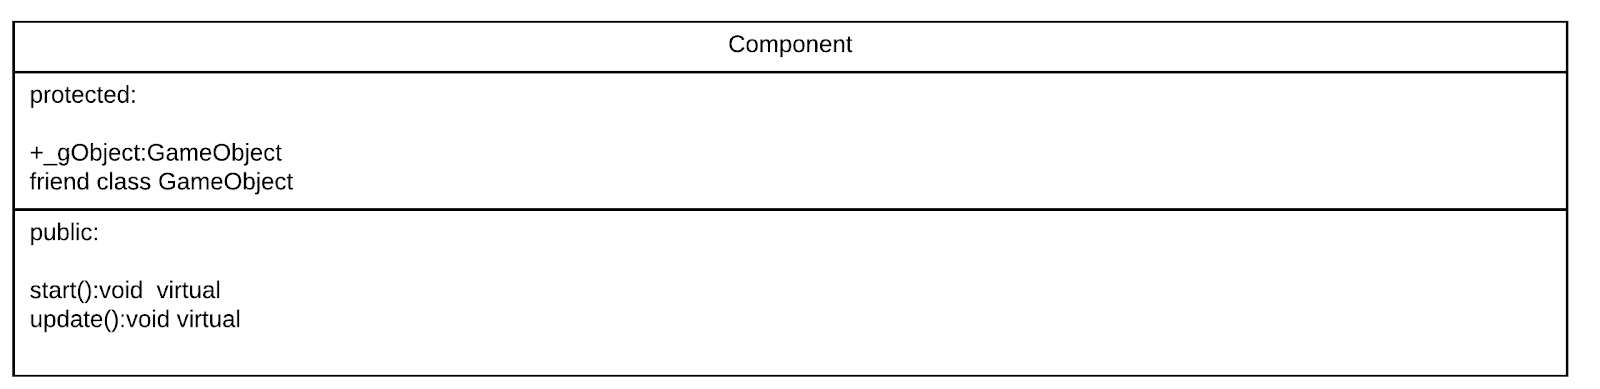
\includegraphics[scale=0.3, keepaspectratio]{img/Component.png}
    \caption{Diagrama de clases de la clase Component}
    \label{figura:Component}
\end{figure}

Dentro de las componentes internas, la clase encargada de almacenar las matrices de posición para la gestión del árbol de escena dentro
del sistema de coordenadas es la componente transformada.

\vspace{1mm} %5mm vertical space

La clase transformada guarda las estructura de datos matriciales que se definen en la librería matemática de OpenGL para posicionar los
objetos en el sistema de coordenadas. La matriz cuenta con una matriz de modelo y otra matriz de modelo global que tienen sentido cuando
se usan en la estructura de datos en árbol, generando dependencias de posición entre objetos de juego dentro del árbol.

\vspace{1mm} %5mm vertical space

Para realizar la recursividad de las transformadas dentro de la propia clase se utiliza un atributo interno que almacena las transformadas
de los objetos de juego hijos de ese objeto de juego y realizar los cálculos matriciales dentro de la clase transformada.

\vspace{1mm} %5mm vertical space

El acceso a las matrices de modelo global y la matriz de modelo se realiza de manera pública por el objeto de juego para realizar operaciones
de rotación, traslación y escalado de las matrices explicadas en la clase objeto de juego.

\begin{figure}[H]
    \centering
    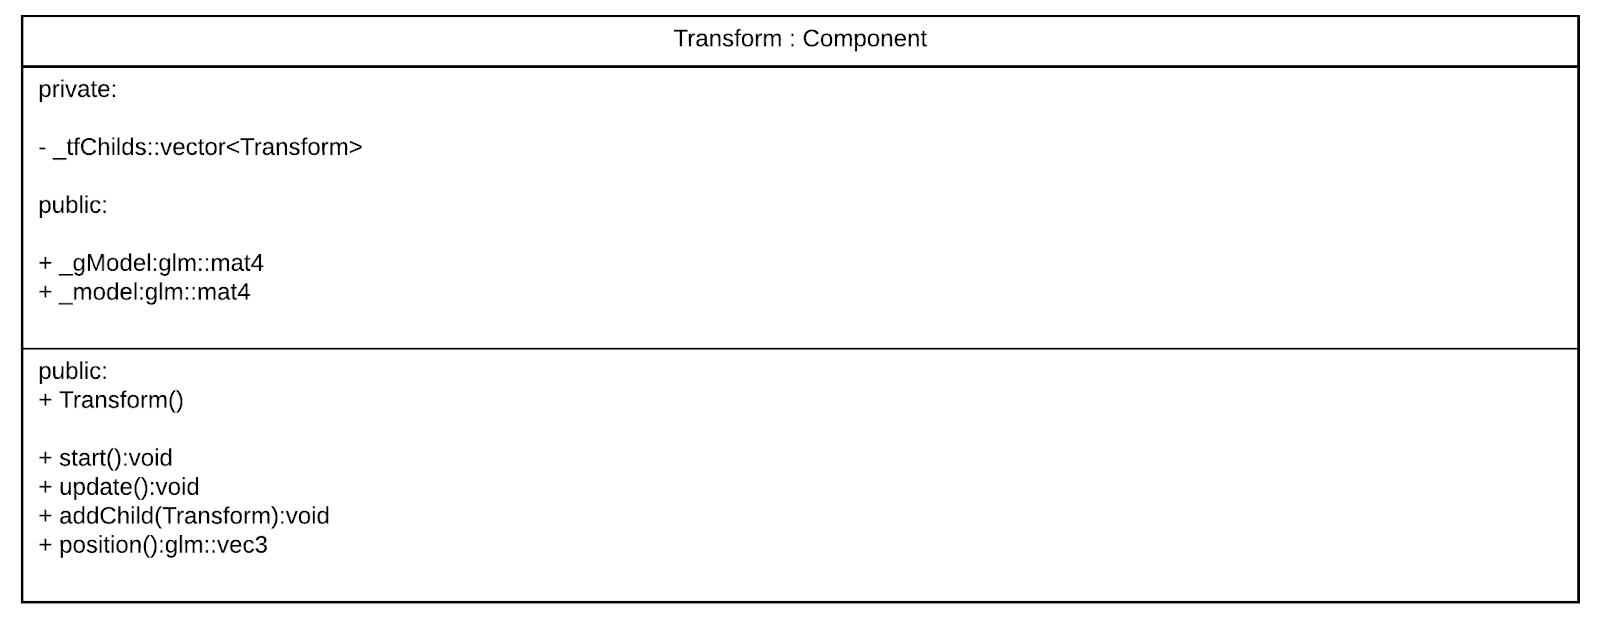
\includegraphics[scale=0.3, keepaspectratio]{img/Transform.png}
    \caption{Diagrama de clases de la clase Transform}
    \label{figura:Component}
\end{figure}

La siguiente clase es la componente cámara, esta componente también almacena una transformada para definir la posición de la cámara en el
sistema de coordenadas de OpenGL y poder realizar los cálculos de la etapa de vértices de los objetos de juego con la posición de la cámara.
Para realizar los cálculos de la etapa de vértices la cámara devuelve su posición invertida para seguir el modelo de proyección de OpenGL.

\vspace{1mm} %5mm vertical space

Esta clase cuenta con propiedades de la cámara para abrir el ángulo de visión y el aspecto de vista panorámico o en cuatro tercios y cambiar
la forma de proyección de la cámara ya sea en modo de perspectiva para escenas en 3D o hacer uso de una cámara ortogonal para 
escenas en 2D.

\begin{figure}[H]
    \centering
    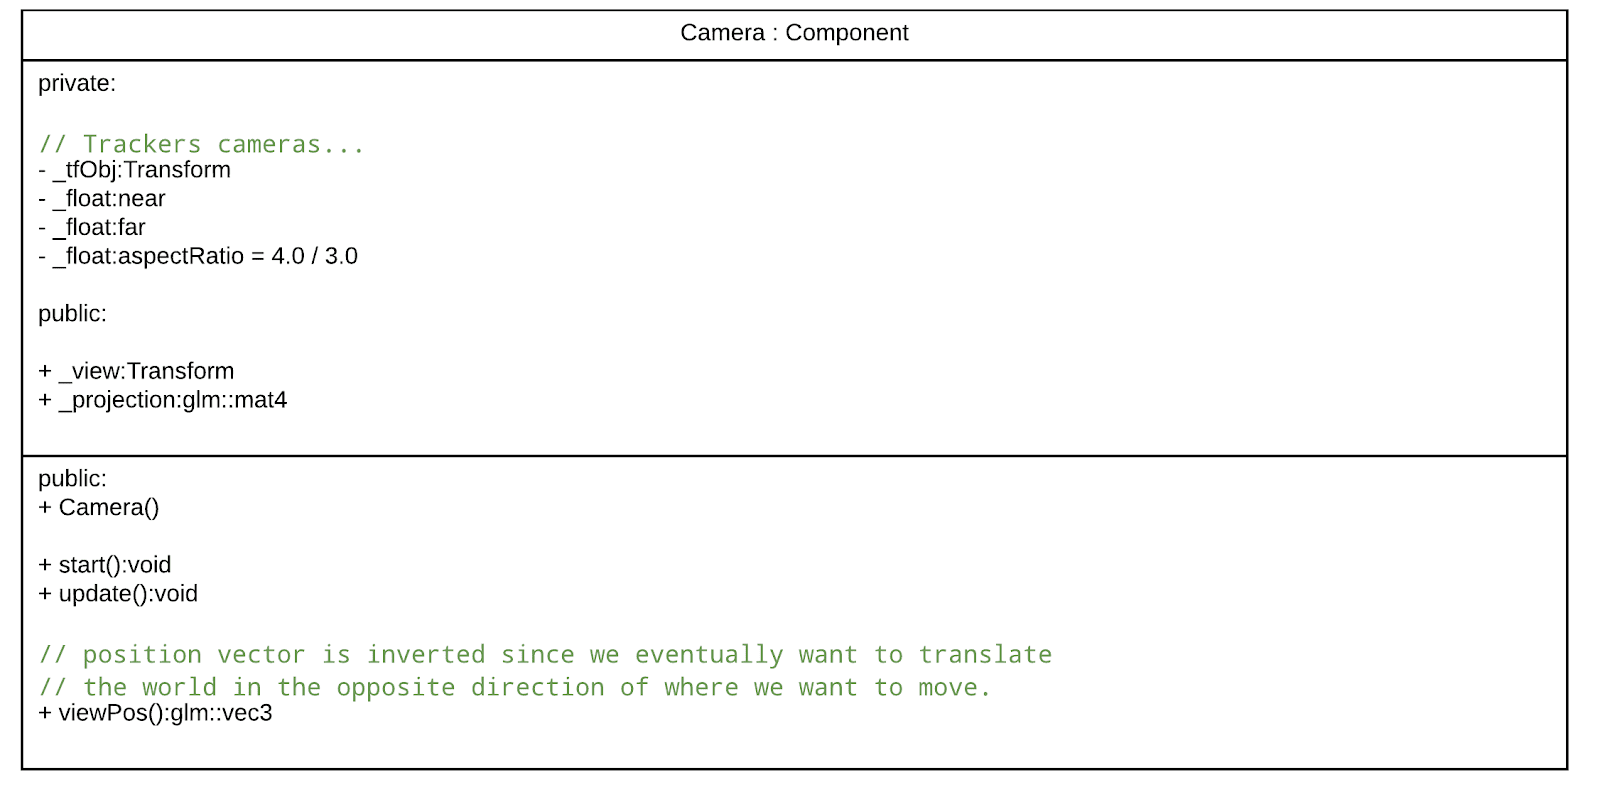
\includegraphics[scale=0.3, keepaspectratio]{img/Camera.png}
    \caption{Diagrama de clases de la clase Camera}
    \label{figura:Component}
\end{figure}

La clase de luces se define como una interfaz en C++, es una clase abstracta con un conjunto de métodos virtuales que implementan cada
tipo de luz, existen luces direccionales, puntuales y focales que heredan de la clase virtual luces.

\vspace{1mm} %5mm vertical space

La clase virtual de luces cuenta con los métodos de posición, dirección, intensidad y distancia que son utilizados por el usuario cada
vez que cree un tipo de luz. Cada uno de los tipos de luz que heredan de la clase luces realizan operaciones en los métodos de la
interfaz teniendo en cuenta su naturaleza.

\vspace{1mm} %5mm vertical space

La clase de luces se define como una interfaz en C++, es una clase abstracta con un conjunto de métodos virtuales que implementan cada tipo
de luz, existen luces direccionales, puntuales y focales que heredan de la clase virtual luces.

\vspace{1mm} %5mm vertical space

La clase virtual de luces cuenta con los métodos de posición, dirección, intensidad y distancia que son utilizados por el usuario cada
vez que cree un tipo de luz. Cada uno de los tipos de luz que heredan de la clase luces realizan operaciones en los métodos de la
interfaz teniendo en cuenta su naturaleza.

\begin{figure}[H]
    \centering
    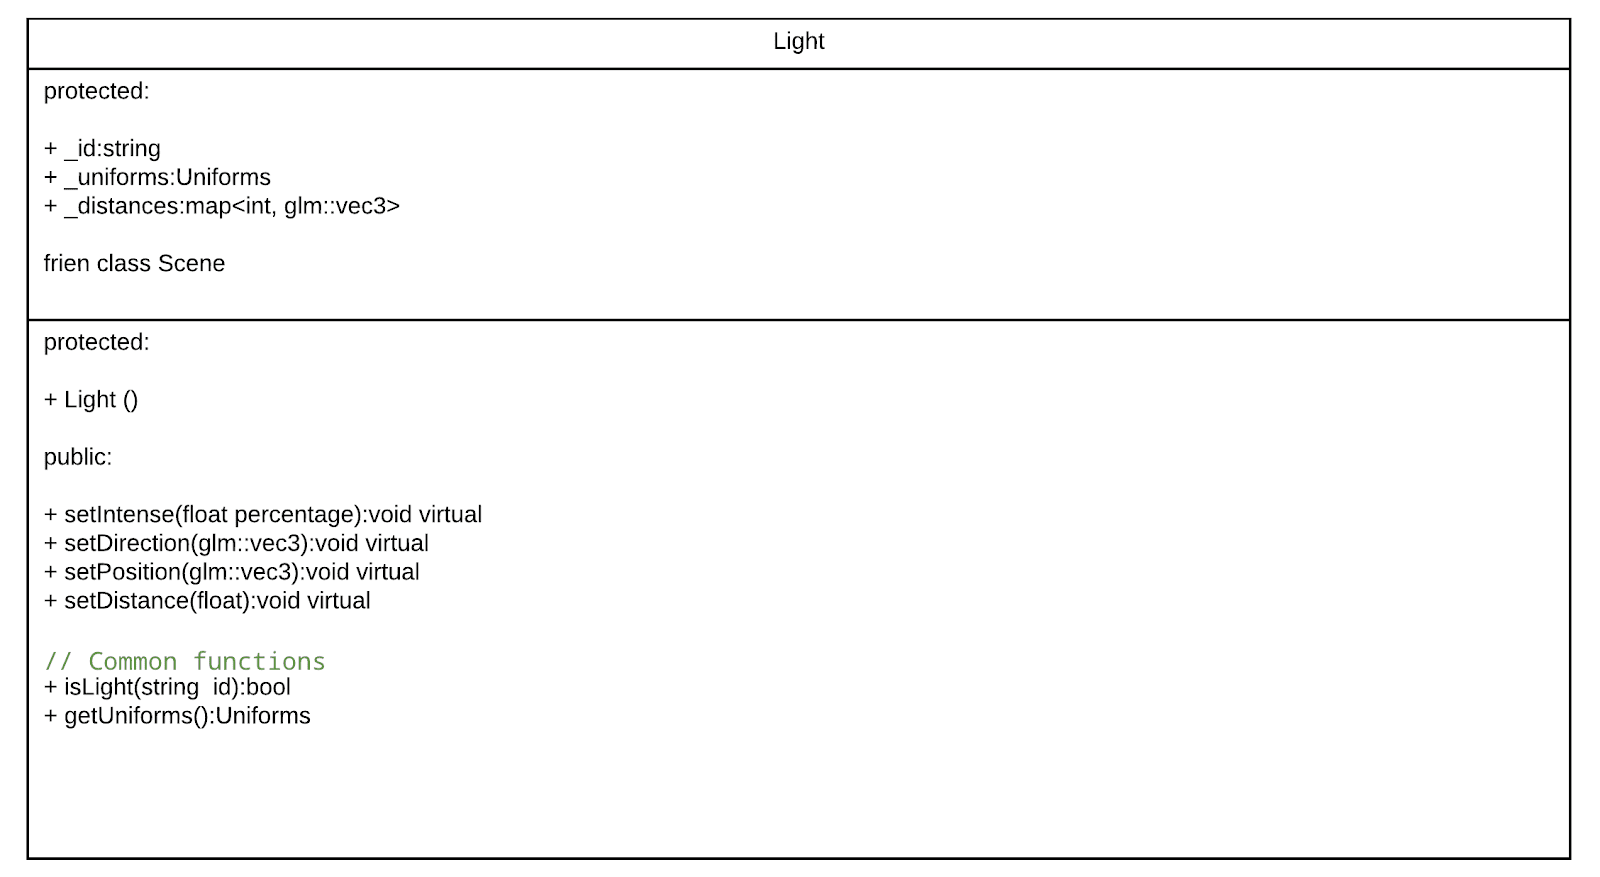
\includegraphics[scale=0.30, keepaspectratio]{img/Litght.png}
    \caption{Diagrama de clases de la clase Litght}
    \label{figura:Component}
\end{figure}

Las técnicas de iluminación utilizadas en el motor realizan técnicas de iluminación local en tiempo real utilizando para ello las
componentes de iluminación del modelo de pong.

\subsection{Modelo de Phong} 
\label{sec:Modelo de Phong}

El modelo de phong es una técnica de iluminación gráfica para simular el comportamiento de las luces en el mundo real, este modelo
cuenta con tres componentes de luz para este propósito; componente ambiental, difusa y especular.

\vspace{1mm} %5mm vertical space

La componente ambiental dará iluminación uniforme a todo el material iluminando las partes del objeto que no son influenciadas por
una fuente de luz de manera directa y poder mostrar la caras ocultas de los objetos.

\vspace{1mm} %5mm vertical space

La componente difusa ilumina las superficies del material que tienen incidencia de manera directa con una fuente de luz, teniendo en
cuenta la dirección y posición de la fuente de luz, esta componente puede sobreescribir la componente ambiental si queremos que las
partes del objeto que no son visibles desde ninguna fuente de luz queden ocultas.

\vspace{1mm} %5mm vertical space

La componente especular da el efecto de brillo sobre el material, este efecto se consigue realizando un cálculo exponencial de reflejo
sobre los fragmentos. La componente especular tiene en cuenta la posición de perspectiva de visión, la posición de la fuente de luz
y la posición del fragmento.

\vspace{1mm} %5mm vertical space

El valor exponencial afectará a la precisión de brillo en el material. Los fragmentos iluminados por la componente especular serán
filtrados por el reflejo y cambiará a medida que se mueva la posición del observador dando un mayor realismo a la iluminación del
material.

\begin{figure}[H]
    \centering
    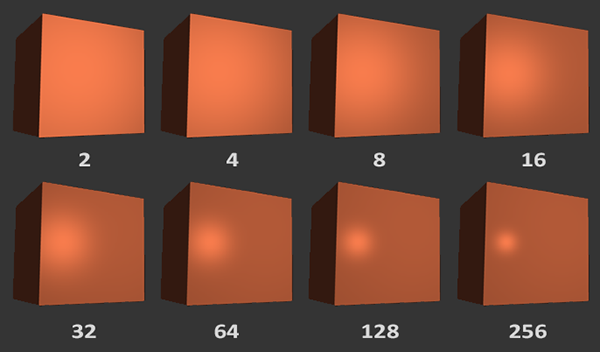
\includegraphics[scale=0.5, keepaspectratio]{img/basic_lighting_specular_shininess.png}
    \caption{Imagen que muestra el modelo de pong con diferentes valores del factor exponencial de la componente especular.}
    \label{figura:Component}
\end{figure}

El usuario podrá añadir un conjunto de luces en la escena haciendo uso del modelo de phong, dispondrá de tres tipos de luces para
iluminar la escena, luces direccionales, luces puntuales y luces de foco. Este conjunto de luces definen el sistema de luces del motor.


\subsection{Sistema de luces} 
\label{sec:Luces}

Las luces direccionales están diseñadas como fuente de luz infinitas, la posición de la luz será descartada y sólo se tendrá en cuenta
la dirección de la luz. Este tipo de luz puede ser útil para simular la iluminación del sol donde todos los objetos son iluminados de
la misma manera independientemente de su posición en la escena respecto a la fuente de luz.

\begin{figure}[H]
    \centering
    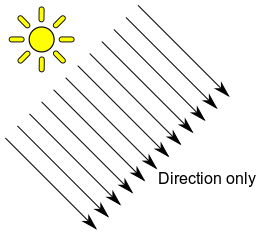
\includegraphics[scale=0.5, keepaspectratio]{img/DirectionalLightDiagram.png}
    \caption{ Diagrama de ejemplo de luz direccional documentación de Unity.}
    \label{figura:Component}
\end{figure}

Las luces puntuales están diseñadas como fuentes de luz que iluminan su entorno de manera uniforme desde su posición, estas fuentes de
luz no tienen dirección. Los objetos son iluminados en la escena teniendo en cuenta la posición de los fragmentos del material respecto
a la posición de la fuente de luz puntual. El usuario podrá generar hasta 255 luces puntuales dentro de la escena y podrá situarlas en
cualquier punto de la escena.

\begin{figure}[H]
    \centering
    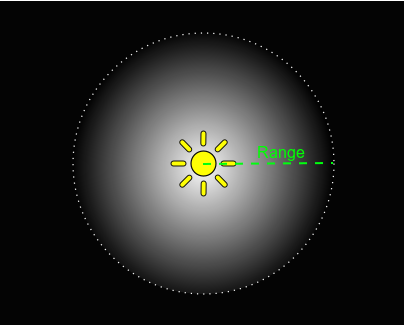
\includegraphics[scale=0.5, keepaspectratio]{img/PointLightDiagram.png}
    \caption{Diagrama de ejemplo de luz puntual documentación de Unity.}
    \label{figura:PointLightDiagram}
\end{figure}

Para poder simular la distancia entre las luces puntuales y los materiales de los objetos se ha diseñado un factor de atenuación. Este factor
de atenuación utiliza una fórmula matemática que decrece de forma cuadrática en función de la distancia entre la fuente de luz y la posición
de los fragmentos del material.

\begin{equation} \label{distance}
F_{att} = \frac{1} {(K_{c} + K_{l} \cdot d + K_{q} \cdot d^2)} [0 , 1]
\end{equation}

La ecuación \ref{distance} calcula la distancia de la fuente de luz al origen de la superificie del material.

\vspace{1mm} %5mm vertical space

Los valores constantes son sacados de una tabla que cambiarán el alcance de las luces puntuales. 

\vspace{1mm} %5mm vertical space

El factor cuadrático de la distancia es utilizado para simular el comportamiento físico de los rayos de luz
en el mundo real. Si se utiliza este valor escalar con valores entre cero y uno en los fragmentos del material
se puede variar el valor de intensidad de iluminación en mayor o menor medida sobre los fragmentos de las superficies.

\vspace{1mm} %5mm vertical space

Las luces de foco simulan un foco de luz, este tipo de luz tiene en cuenta su posición y el ángulo de apertura
del foco. El motor puede simular una luz de foco para iluminar la escena. El usuario podrá configurar el alcance
de la luz de foco con el factor de atenuación y su ángulo de apertura. Para realizar un mayor realismo de la
luz de foco existe un parámetro de cutoff que se utiliza para simular los bordes de iluminación del foco de luz.

\begin{figure}[H]
    \centering
    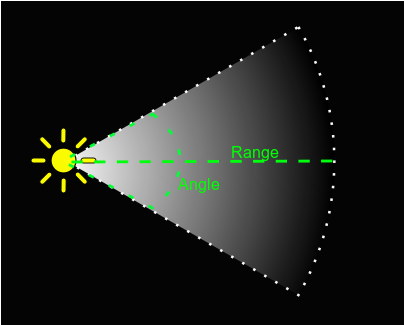
\includegraphics[scale=0.5, keepaspectratio]{img/SpotLightDiagram.png}
    \caption{Diagrama de ejemplo de luz puntual documentación de Unity.}
    \label{figura:SpotLightDiagram}
\end{figure}

Una vez explicadas las técnicas de iluminación de la escena el siguiente paso es explicar las clases internas
que determinan los objetos de juego renderizables.

\vspace{1mm} %5mm vertical space

Existe una clase específica Drawer para definir el comportamiento de las componentes renderizables del motor.
Esta clase cuenta con tres atributos virtuales re definibles; activación, dibujado y añadir vista. Estos tres
atributos definen el comportamiento de las clases renderizables del motor. Todas las clases renderizables contarán
por defecto con la clase programa y la clase uniformes.

\begin{figure}[H]
    \centering
    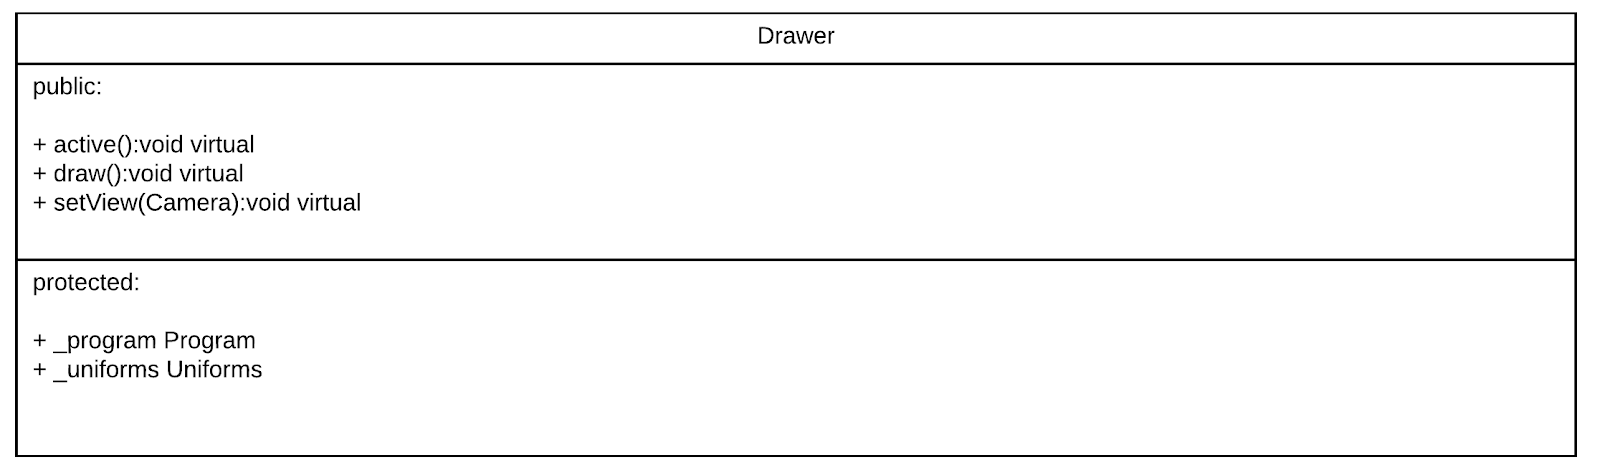
\includegraphics[scale=0.25, keepaspectratio]{img/Drawer.png}
    \caption{Diagrama de clases de la clase Drawer}
    \label{figura:Drawer}
\end{figure}

La componente renderizable que hereda de la clase Drawers almacena la clase de modelo y las funciones para saber si el
modelo renderizable es o no transparente para el momento del encolado de los objetos de juego y su renderización. Además
cuenta con una función para añadir la matriz de modelo del objeto de juego en la renderización y posicionar de forma
correcta el objeto renderizado en la escena.

\vspace{1mm} %5mm vertical space

La clase de renderizado cuenta con un método para actualizar el sistema de luces en la escena y de esta manera poder mover
la iluminación en los objetos de juego renderizables en tiempo real.

\vspace{1mm} %5mm vertical space

Los objetos renderizables contarán con clases internas del motor gráfico para definir las geometrías y los materiales que
serán utilizados en las etapas de vértices y de fragmentos del cauce gráfico.

\begin{figure}[H]
    \centering
    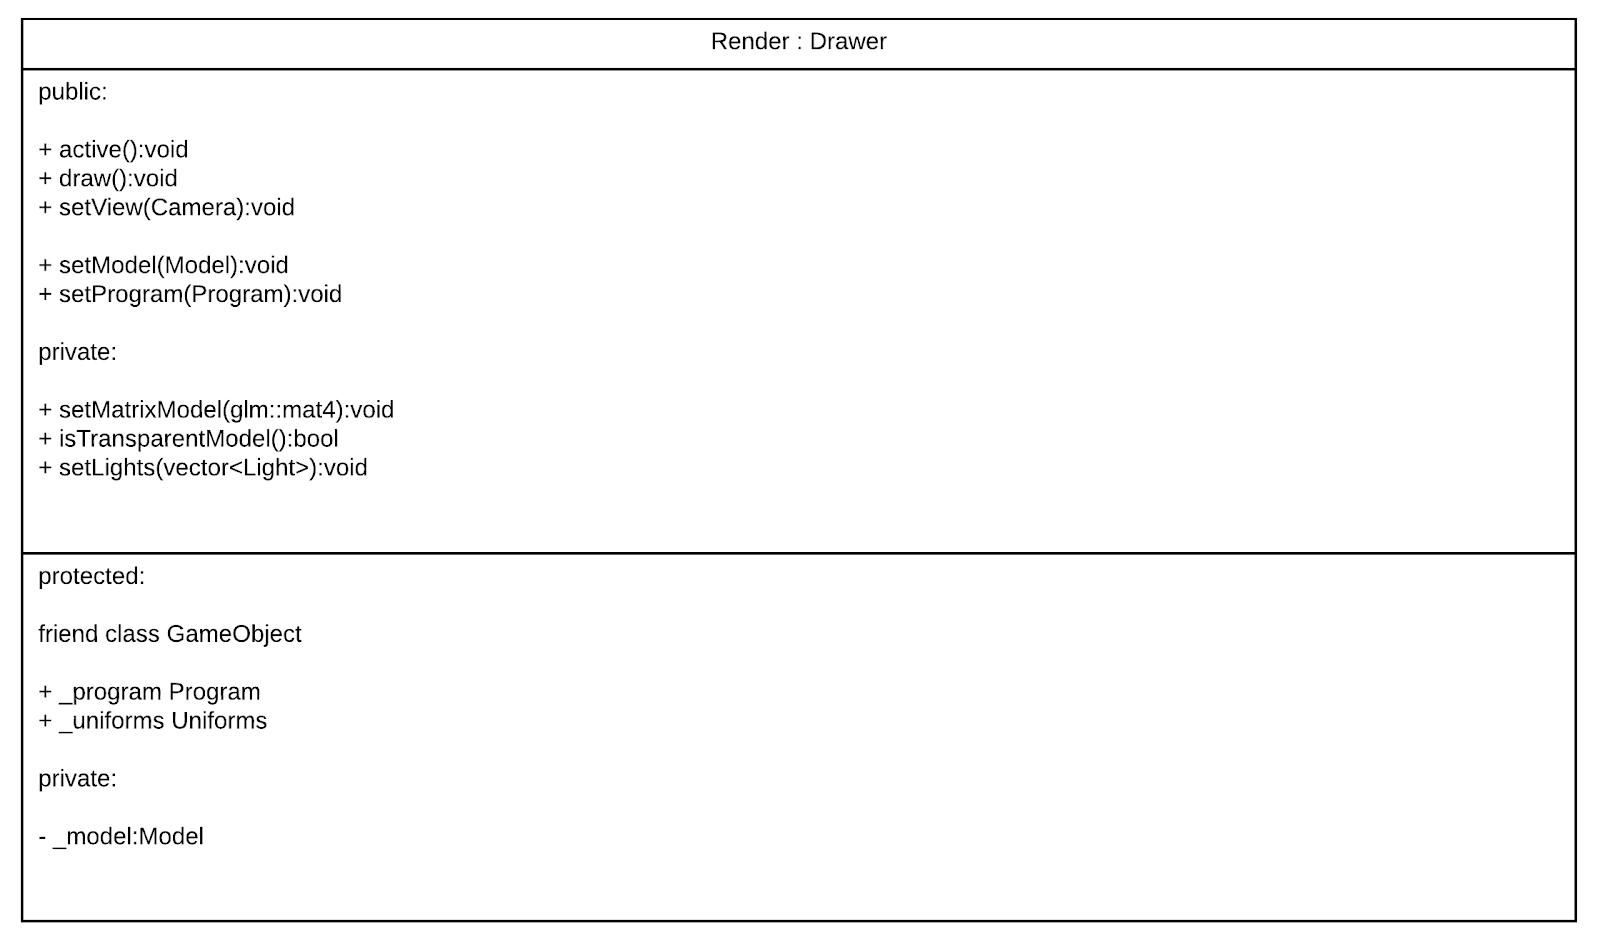
\includegraphics[scale=0.25, keepaspectratio]{img/Render.png}
    \caption{Diagrama de clases de la clase Render}
    \label{figura:Render}
\end{figure}

La clase de alto nivel que abstrae de las etapas del cauce gráfico como se puede ver en la definición de la clase de renderizado es
la clase modelo que se define a continuación.

\vspace{1mm} %5mm vertical space

La clase modelo almacena el conjunto de geometrías, cada una de las geometrías que componen el modelo son almacenadas en la clase
malla. La clase modelo ya no es una componente del objeto de juego ya que la componente es la clase renderizable que identifica
si un objeto de juego es o no renderizable y debe pasar por el cauce gráfico. 

\vspace{1mm} %5mm vertical space

La clase modelo almacena una colección de mallas que almacenan las estructuras de datos de los vértices y las propiedades del
material de cada malla. Incluyendo la definición de las texturas que se almacenan en la clase material.

\vspace{1mm} %5mm vertical space

Para la realización de carga de modelos complejos, la clase modelo almacena el directorio donde se encuentra el modelo y una clase
de métodos internos para cargar un modelo compuesto de varias geometrías y cargar las texturas del material de cada geometría.

\vspace{1mm} %5mm vertical space

Esta clase contiene el acceso a la librería Assimp, librería utilizada en el motor para realizar la conversión de archivos de otras
plataformas gráficas a datos entendibles por OpenGL, internamente la clase contiene métodos para el procesamiento de los datos
recibidos por la librería Assimp y almacenarlos en las estructuras de datos del motor gráfico. 

\vspace{1mm} %5mm vertical space

Existen una serie de métodos de la clase modelo accesibles por la clase de renderizado para definir las etapas de cauce, activación
y dibujado.

\begin{figure}[H]
    \centering
    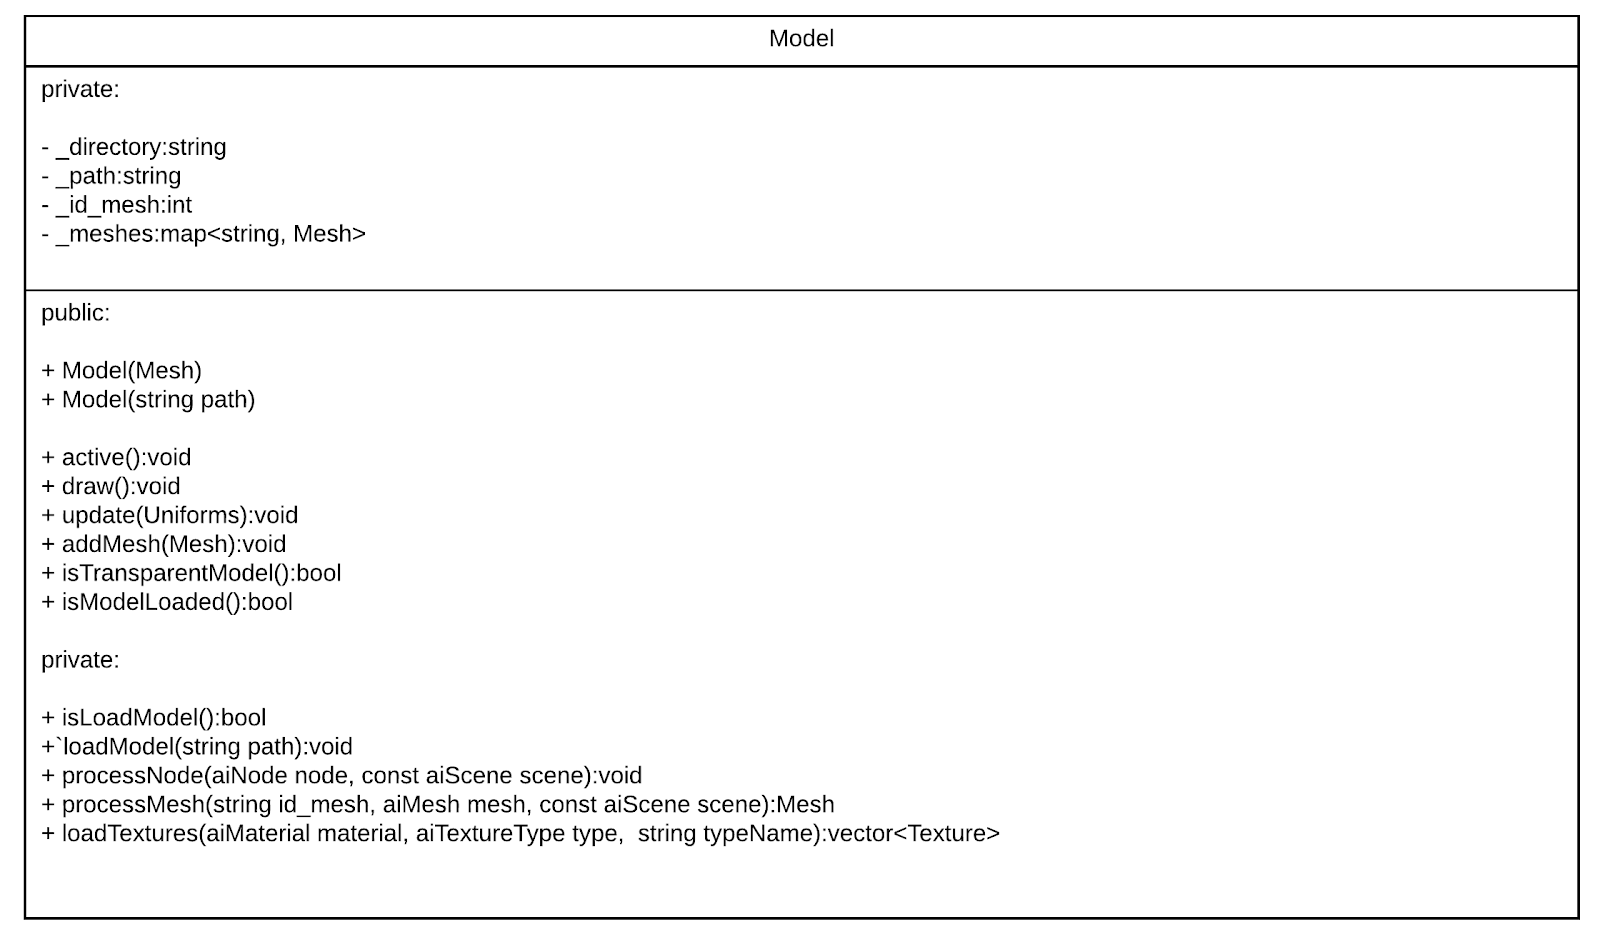
\includegraphics[scale=0.25, keepaspectratio]{img/Model.png}
    \caption{Diagrama de clases de la clase Model}
    \label{figura:Model}
\end{figure}

La clase material contiene los datos del  programa de shaders de la etapa de fragmentos estos datos se definen en una estructura de
datos común para todos los programas de shaders de la etapa de fragmentos del motor gráfico.

\begin{figure}[H]
    \centering
    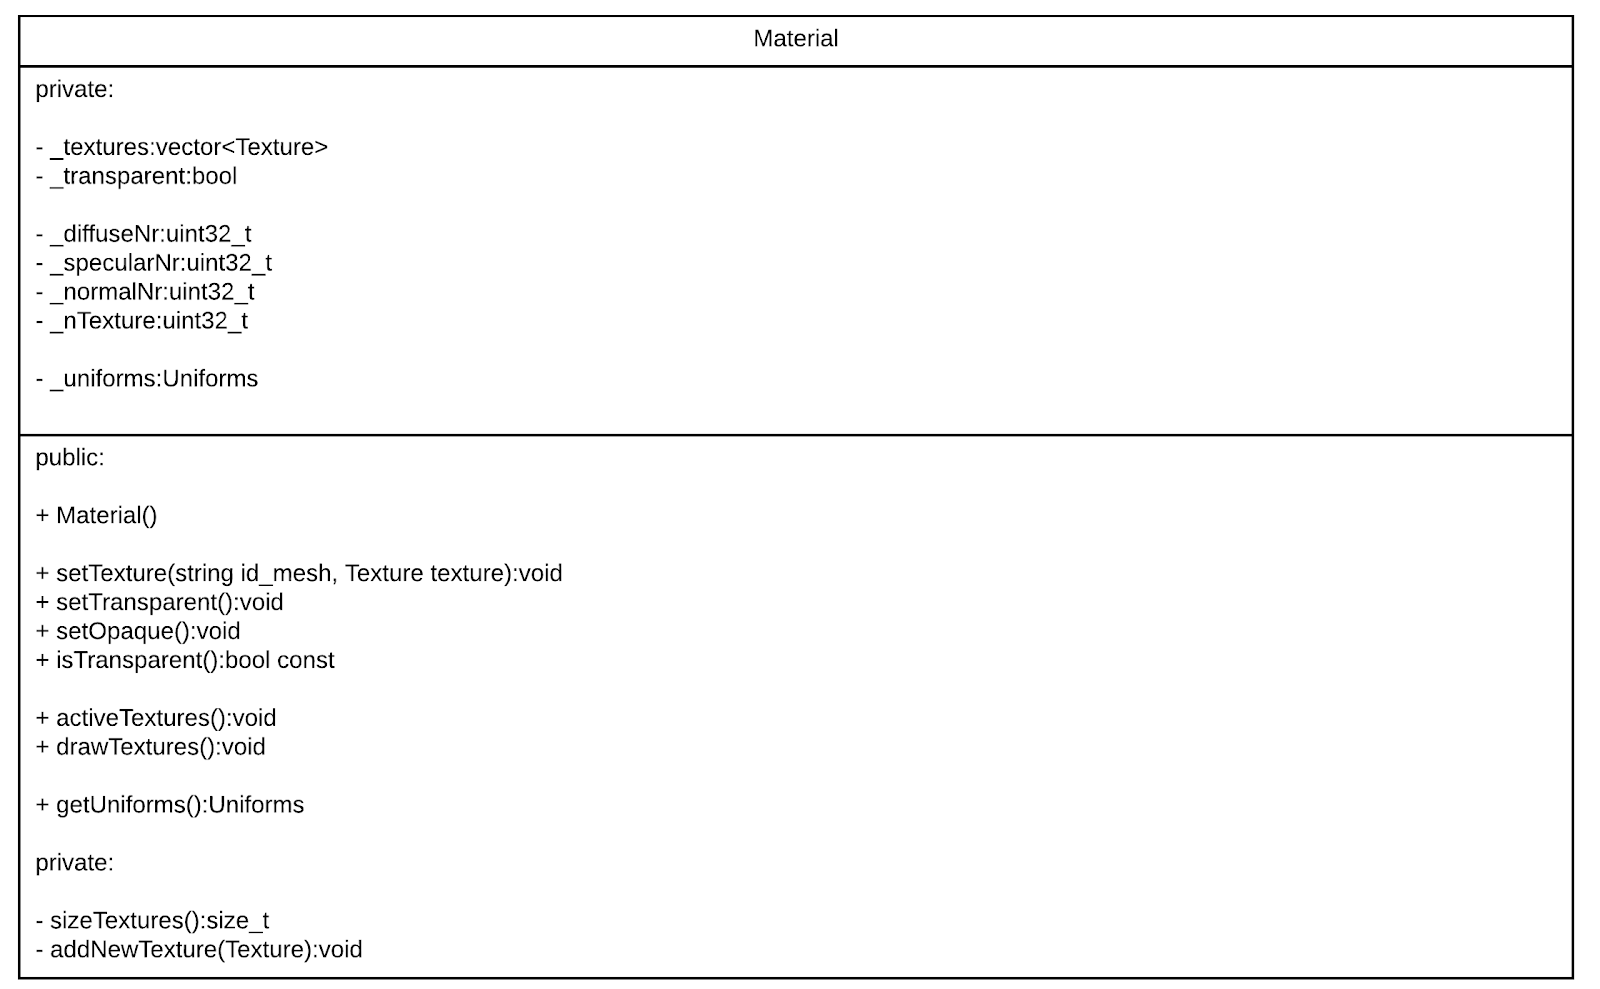
\includegraphics[scale=0.25, keepaspectratio]{img/Material.png}
    \caption{Estructura de datos de material definido en el motor gráfico etapa de fragmentos}
    \label{figura:Material}
\end{figure}

Esta estructura de datos almacena una colección de texturas difusas, especulares y normales. El material puede hacer uso de una o
varias texturas para definir las superficie del material. Además haciendo uso de los programas de shaders de usuario, puede definir
diferentes comportamientos de los fragmentos de forma específica haciendo uso de las texturas definidas en el material de la malla.

\vspace{1mm} %5mm vertical space

La clase de materiales podrá activar y dibujar las texturas del material o decidir si la malla renderizable es o no transparente para
las técnicas de blending del motor. 

\vspace{1mm} %5mm vertical space

Esta clase tiene su propia clase de uniformes donde se almacena la estructura de datos de la variable uniforme del programa de shaders
de cualquier material del motor. En esta clase también se almacena la colección de texturas que definen el material del motor para
su posterior renderizado.

\begin{figure}[H]
    \centering
    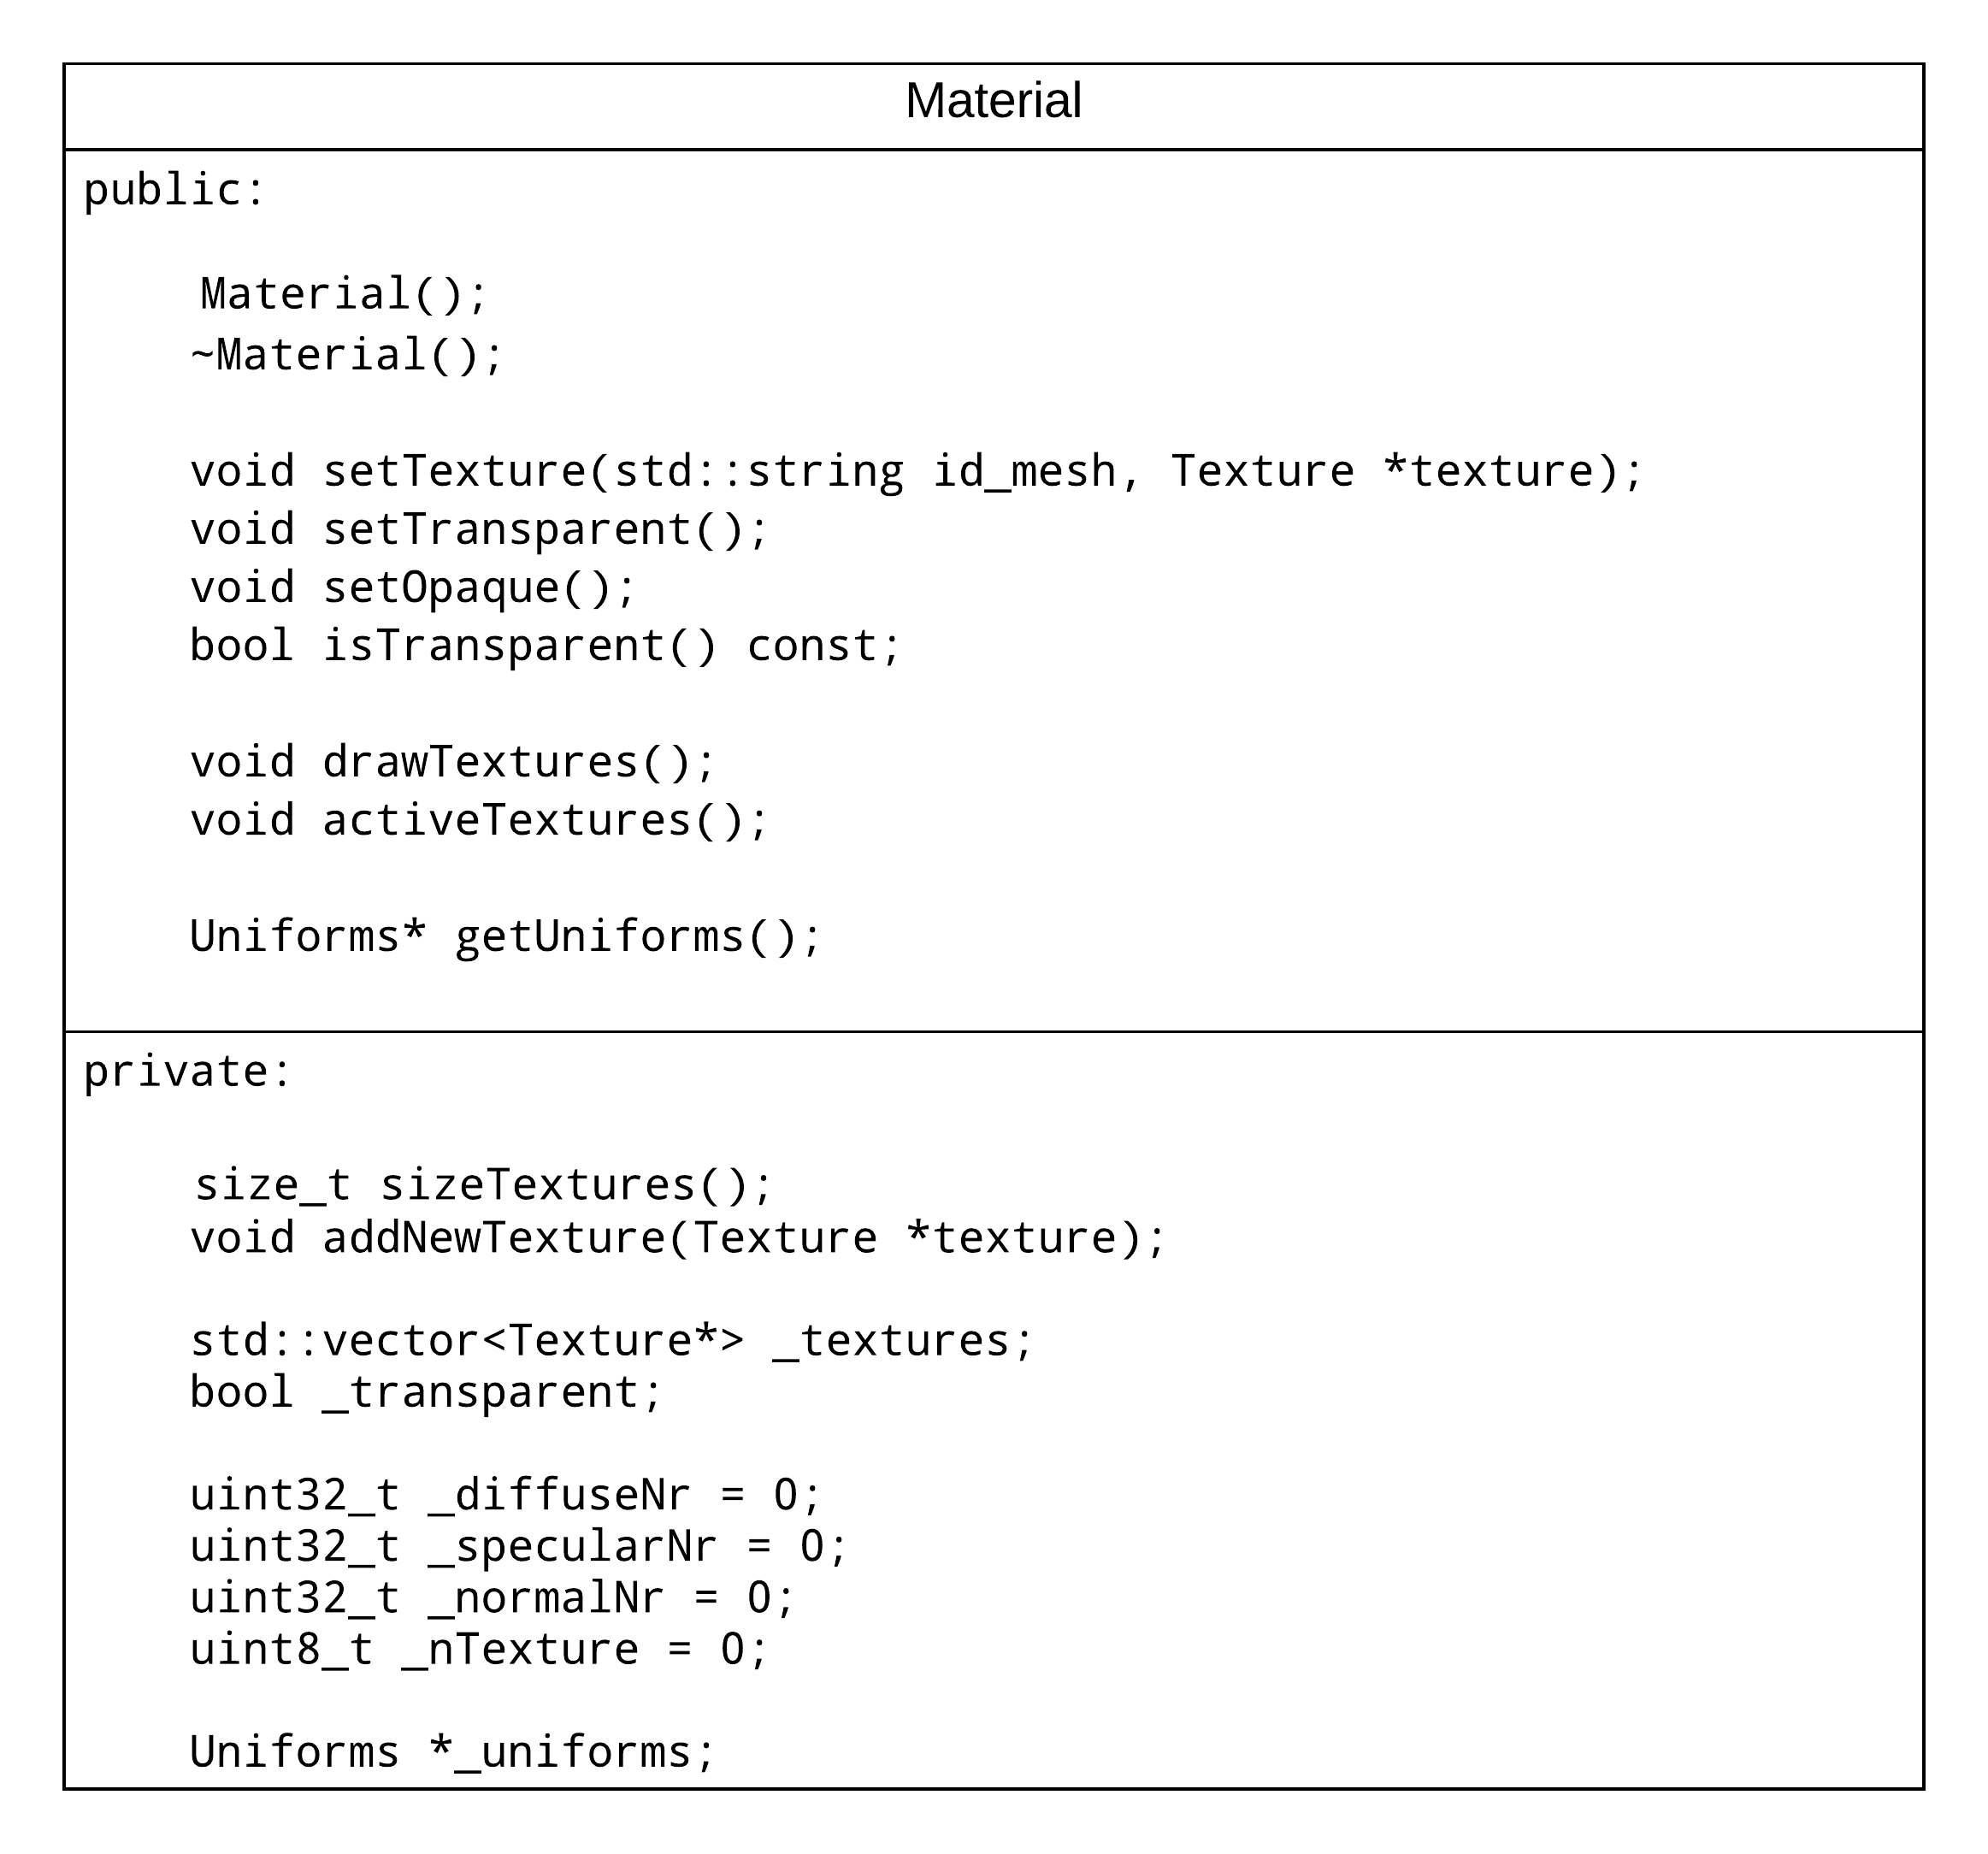
\includegraphics[scale=0.5, keepaspectratio]{img/material_class.png}
    \caption{Diagrama de clases de la clase Material}
    \label{figura:material_class}
\end{figure}

La clase modelo generará los valores de las texturas de la estructura de datos de material de forma dinámica en función del número de
texturas que definen el material de la malla.

\vspace{1mm} %5mm vertical space

La siguiente definición de clases de bajo nivel almacena los datos del contexto de OpenGL y su máquina de estados y el acceso a la
interfaz de la librería gráfica de OpenGL, comenzando con la clase de texturas y los tipos de texturas.

\subsection{Tipos de texturas}
\label{subsec:Texturas}

La clase texturas contiene el identificador de texturas del contexto de OpenGL, cuenta con una constante para definir el directorio
donde se almacenan las texturas de un proyecto realizado con el motor gráfico, directorio resources. Este directorio debe almacenar el
nombre del archivo de la imagen 2D para generar la textura. A no ser que la textura sea cargada desde Assimp utilizando un fichero
con extensión .mtl.

\vspace{1mm} %5mm vertical space

La clase de texturas cuenta con dos métodos estáticos para cargar las texturas del directorio que se especifique como parámetro la ruta
de la imagen 2D de la textura y almacenarla en el contexto de OpenGL. 

\begin{figure}[H]
    \centering
    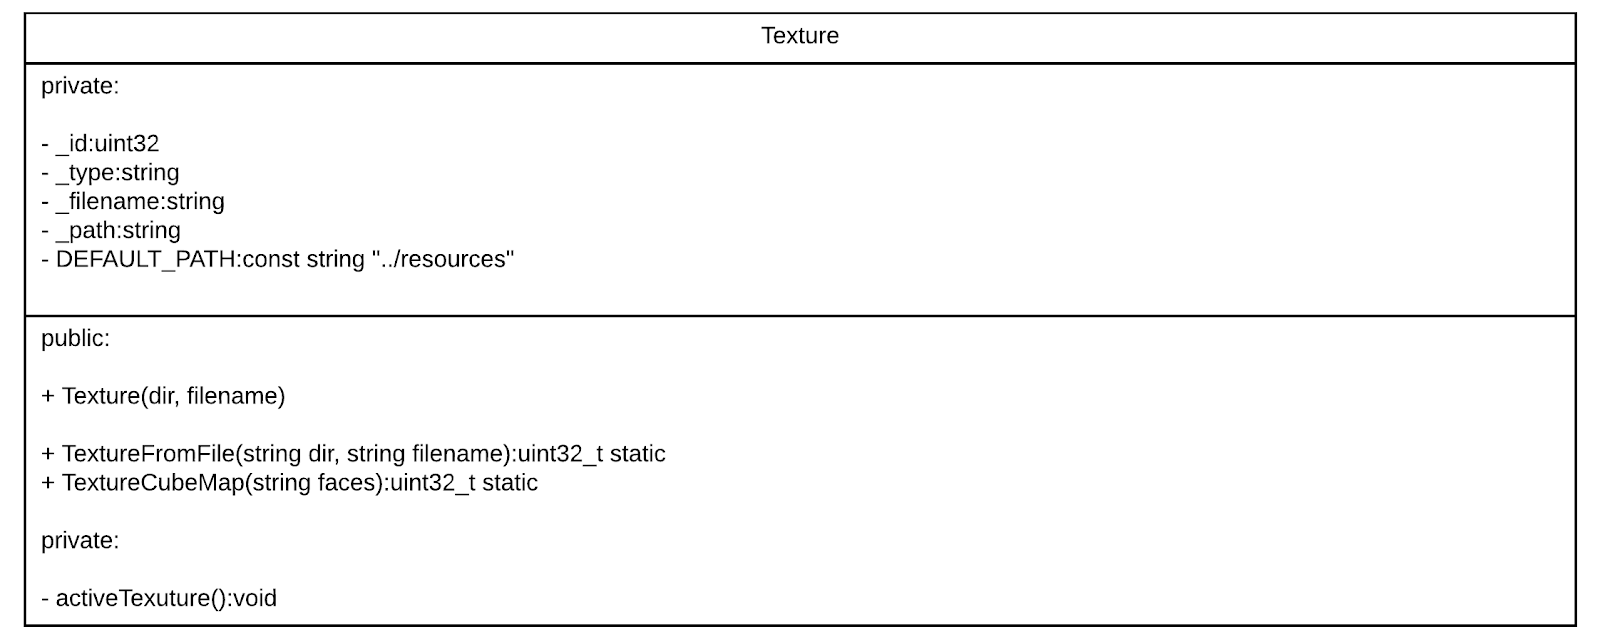
\includegraphics[scale=0.25, keepaspectratio]{img/Texture.png}
    \caption{Diagrama de clases de la clase Texture}
    \label{figura:Texture}
\end{figure}

Existen tres tipos de texturas dentro del motor; texturas difusas, especulares y normales.

\vspace{1mm} %5mm vertical space

Las texturas difusas definen el material básico y los colores de la superficie para los programas de la etapa de fragmentos. Estas
texturas reaccionan ante una componente de luz difusa siguiendo el modelo de phong.

\vspace{1mm} %5mm vertical space

Las texturas especulares definen las partes brillantes del material desde la perspectiva de la cámara reaccionando sobre la componente
especular del modelo de pong.

\vspace{1mm} %5mm vertical space

Las texturas normales cambiarán la dirección de los vectores de las componentes normales de la superficie del material en la etapa de
fragmentos dando la sensación de rugosidad sobre la superficie del material obteniendo un coste de rendimiento menor que definiendo
esta rugosidad en la geometría del modelo.

\begin{figure}[H]
    \centering
    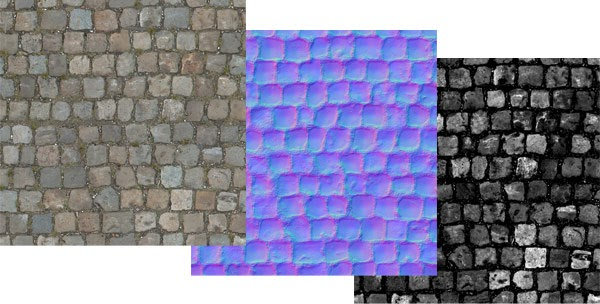
\includegraphics[scale=0.45, keepaspectratio]{img/custom-textures.jpg}
    \caption{Imagen con la definición de los tipos de texturas del motor, difusa, normal y especular de izquierda a derecha.}
    \label{figura:Texture}
\end{figure}

Una vez definido el material la siguiente clase de bajo nivel almacena las geometrías de las etapas previas a la etapa de ensamblado y
realizando la especificación de vértices de manera transparente para el usuario.

\vspace{1mm} %5mm vertical space

La clase malla almacena el nombre de la malla a modo de identificador, este identificador es usado por la clase modelo para acceder
a las mallas del modelo. 

\vspace{1mm} %5mm vertical space

La clase malla contiene todas las funciones de OpenGL para el renderizado de los objetos e iniciar el cauce gráfico, por esta razón
contiene los identificadores del contexto de OpenGL una vez definidos en la etapa de especificación de vértices VAO VBO y EBO. Estos
identificadores son devueltos por la librería de OpenGL una vez enviados los datos de primitivas almacenados por la clase malla.
También cuenta con la referencia a la clase de uniformes y la clase de programa para realizar la activación del cauce.

\vspace{1mm} %5mm vertical space

La clase malla tiene estructurados los atributos de la especificación de vértices en dos vectores uno que almacena los índices de
orden de ensamblado de las primitivas y otro vector con los atributos de normales posición de vértices y coordenadas de texturas
definidas en la estructura de datos Vertex.

\vspace{1mm} %5mm vertical space

La malla contiene el vector de texturas que componen en el material de la geometría para su activación en el contexto de OpenGL.
Esta colección de texturas contará con las texturas del material definidas anteriormente, normal, difusa y especular.

\vspace{1mm} %5mm vertical space

Existen un conjunto de métodos de la clase malla accesibles por la clase modelo para activar y renderizar las mallas del modelo
y sus texturas en las diferentes etapas del cauce gráfico.

\vspace{1mm} %5mm vertical space

El resto de atributos de la clase malla son utilizados para comunicarse con la librería de OpenGL, realizar la especificación de
vértices y cambiar la máquina de estados de OpenGL antes del renderizado para realizar las técnicas de blending. Los métodos de
blending son accesibles por la clase modelo ya que esta clase es la que tiene que decidir si el modelo es transparente u opaco
para la ordenación de los objetos de juego en el renderizado. 

\vspace{1mm} %5mm vertical space

La clase malla tendrá acceso a las clases de bajo nivel de comunicación con las etapas programables del cauce para poder activar
los programas de la malla que se quiera realizar su renderizado.

\vspace{1mm} %5mm vertical space

La clase uniformes realiza la abstracción de la librería matemática de OpenGL contiene una serie de mapas con los tipos de datos
primitivos de la librería matemática. Los mapas utilizarán el nombre de la variable como clave y el valor el tipo de dato primitivo
de la librería matemática de OpenGL; entero, flotante, vectorial de tres y cuatro dimensiones o matricial de tres o cuatro dimensiones. 

\vspace{1mm} %5mm vertical space

Esta clase almacena los datos de los programas de cada malla para facilitar la actualización de los datos de los programas de
shaders de cada malla y sus materiales. Cada malla tendrá una instancia de uniformes con los datos de los programas de vértices
y fragmentos de esa malla.

\vspace{1mm} %5mm vertical space

La clase de programas almacena las instrucciones de los programas de la etapa de vértices y fragmentos, almacena los identificadores
de los dos programas devueltos por el contexto de OpenGL y un mapa de nombres de la variables uniformes como clave y valor el
identificador de la variable devuelto por el contexto de OpenGL en el momento de su creación.

\vspace{1mm} %5mm vertical space

La clase programas además cuenta con las funciones para cargar las estructuras de datos comunes del motor gráfico y las funciones
auxiliares para facilitar al usuario las técnicas de iluminación. En la carpeta utils del motor se encuentran las estructuras de
datos del material ya explicados y las estructuras de datos de las luces básicas además de las funciones para añadir a los fragmentos
de la malla los valores de iluminación de forma correcta.

\vspace{1mm} %5mm vertical space

Al generar los programas de shaders de usuario, estos pueden ser cargados desde un fichero de texto o utilizando un string hardcodeado
dentro de su interfaz de programación.

\vspace{1mm} %5mm vertical space

El usuario podrá crear sus propias variables uniformes en su programa de shaders y estas serán leídas por el motor para añadirlas de
forma correcta en el contexto de OpenGL. El motor filtra las líneas del programa de shader y parsea el nombre y tipo de las variables
uniformes añadiendo la variable al mapa de uniformes del motor y posteriormente realizar su declaración y añadir un valor que será
actualizado en el programa de shaders correspondiente definido por el usuario.

{\Large Sintaxis declaración variables uniformes:  [uniform]    [type]    [name];\par}

La primera palabra es una palabra reservada del lenguaje de shaders de GLSL. La segunda palabra especifica el tipo de variable. El motor
será capaz de interpretar los tipos básicos del lenguaje; float, int, vec2, vec3, vec4, mat3 y mat4. Qué son los valores que puede mapear
la clase uniformes. 

\subsection{Skybox}
\label{subsec:Skybox}

La arquitectura cuenta con una clase de mapa de cubos esta clase es utilizada para simular un entorno dentro de la escena. 

\vspace{1mm} %5mm vertical space

El conjunto de atributos de la clase contienen los identificadores del buffer de vértices del cubo generado internamente y
los nombres de las texturas que componen las texturas internas que componen el entorno como se puede ver en la siguiente imagen.

\begin{figure}[H]
    \centering
    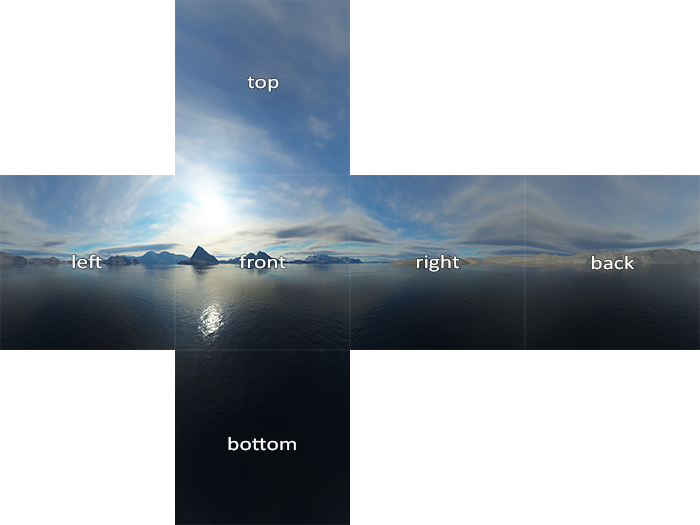
\includegraphics[scale=0.20, keepaspectratio]{img/cubemaps_skybox.png}
    \caption{Ejemplo de textura utilizada para generar el fondo de una escena dentro del motor.}
    \label{figura:cubemaps_skybox}
\end{figure}

La clase Skybox también cuenta con una serie de métodos privados para generar el programa de shaders del Skybox y almacenar la cámara
activa y utilizarla en la fase de renderizado.

\vspace{1mm} %5mm vertical space

El motor generará de forma interna el programa de shaders necesario para generar un mapa cúbico dentro de la escena. El usuario únicamente
definirá un objeto de juego al que añadirá un Drawer de tipo Skybox al objeto de juego y posteriormente será renderizado en la escena con
los ficheros de las texturas que forman el cubo definidos por el usuario.

\vspace{1mm} %5mm vertical space

Para terminar la fase del modelo estático del motor existe una clase de geometrías esta clase es una clase abstracta de la que heredan el
conjunto de geometrías básicas soportadas por el motor. 

\vspace{1mm} %5mm vertical space

La clase abstracta de geometrías define un método que deben implementar todas las geometrías básicas para devolver la malla de la geometría
básica. Existen tres tipos de geometrías básicas; planos, esferas y cubos que el usuario podrá utilizar para renderizar objetos de juego con
geometrías básicas dentro de la escena.

\vspace{1mm} %5mm vertical space

Para realizar los eventos de teclado y reloj existen dos clases, cada una de ellas genera una instancia única dentro de la clase Engine las
instancias de las clases teclado y reloj serán visibles por la interfaz de usuario para trabajar con el teclado y el reloj del motor desde fuera.

\vspace{1mm} %5mm vertical space

La clase teclado cuenta con un método estático que será utilizado por la clase motor para activar el polling de entrada de datos del teclado
usando este método como manejador, con ayuda de las funciones de GLFW para este propósito.

\vspace{1mm} %5mm vertical space

Como fase final de la definición de clases del motor se presenta un diagrama de clases, con los atributos de cada clase y sus dependencias
dentro de la arquitectura.

\section{Definición dinámica de ejecución del motor}
\label{sec:Dinamica}

Una vez explicado el modelo estático del motor la siguiente fase consiste en entender el modelo dinámico o de ejecución controlado por la
clase escena; en sus diferentes etapas de definición, activación, actualización y renderizado.

\subsection{Etapa de definición}
\label{subsec:definicion}

Antes de realizar la ejecución del motor el usuario hará uso de la API para definir una escena, esta etapa previa de definición por el usuario,
define el árbol de escena y las dependencias entre los objetos de juego. 

\vspace{1mm} %5mm vertical space

En esta etapa también se definen las componentes de los objetos de juego su posición inicial o el uso de componentes externas que serán añadidas
al objeto de juego. Se realiza la decisión de qué objetos son renderizables con la componente renderizable y en caso de que el objeto de juego
sea renderizable se añaden las instancias del material, texturas modelo y mallas del modelo. Una vez añadidos los datos de renderizado el usuario
añade la componente de renderizado al objeto de juego. 

\vspace{1mm} %5mm vertical space

Finalizada la etapa de definición el usuario añadirá la escena en el constructor del motor y llamará a los métodos de inicialización y bucle
principal del motor. En esta última llamada el programa se quedará ejecutando en el bucle principal hasta que el usuario cierre la ventana de
OpenGL con algún evento de teclado.

\vspace{1mm} %5mm vertical space

Finalizada la llamada al bucle principal por el usuario, el motor primero ejecutará la etapa de activación, una vez finalizada la inicialización
el motor entrará dentro del bucle principal y realizará las etapas de actualización y renderizado por cada vuelta del bucle.

\subsection{Etapa de activación}
\label{subsec:activacion}

En la primera fase de activación la clase motor generará un contexto de OpenGL y una ventana asociada al contexto donde se realizará el renderizado
de los objetos.

\vspace{1mm} %5mm vertical space

En esta etapa la primera fase es llamar al método de inicialización de la escena. Esta llamada generará la inicialización de todos los objetos
de juego desde el objeto raíz de manera recursiva.

\vspace{1mm} %5mm vertical space

Cada objeto de juego realizará la llamada al método de activación de las componentes y una vez acabado llamará al objeto de inicialización
de sus objetos hijos.

\vspace{1mm} %5mm vertical space

En las componentes internas se realiza la funcionalidad específica de cada componente empezando por la componente de transformadas
encargada del posicionamiento de los objetos en la escena.

\vspace{1mm} %5mm vertical space

Esta activación de posicionamiento de los objetos de la componente transformada define la posición inicial de los objetos de juego
dentro de la escena. En caso de tener objetos de juego estáticos la activación de una componente externa del objeto de juego que
defina esta posición inicial mantendrá al objeto de juego en su posición inicial durante todo el procesamiento de la escena.

\vspace{1mm} %5mm vertical space

Las cámaras se inicializan por defecto en un valor (0,0,5) del sistema de coordenadas de OpenGL para poder visualizar los objetos que
se encuentren en el origen del sistema de coordenadas y mantener una distancia respecto a los objetos de juego que tengan una componente
cámara simulando una visión en tercera persona del objeto de forma inicial.

\vspace{1mm} %5mm vertical space

Los Drawers realizan la inicialización de objetos renderizables para la preparación del cauce gráfico. Tanto la clase renderizable
como la clase de Skybox realizan en la primera etapa del cauce la especificación de vértices y la activación de los programas de
shaders en el contexto de OpenGL.

\vspace{1mm} %5mm vertical space

La clase Skybox realizará la activación del programa de shaders, la carga de la geometría cúbica y las texturas que simulan el entorno
definido por el usuario. Al cargar la textura del cubo de mapa se indica a OpenGL que se tratan de texturas de cubo que se renderizan
en las partes internas de la superficie de la geometría. Una vez cargadas la texturas de las caras del cubo se termina la parte de
activación del Skybox.

\vspace{1mm} %5mm vertical space

En la activación de los objetos renderizables, se comprueba que el objeto cuente con un modelo y un material para su renderizado,
una vez realizada esta comprobación se realiza la activación del modelo. 

\vspace{1mm} %5mm vertical space

La activación del modelo comprobará todas las mallas del objeto y realizará la asociación de texturas y programas de shaders de cada
malla del modelo, finalizando con la activación de la geometría y texturas de cada malla.

\vspace{1mm} %5mm vertical space

En la activación de la malla se realiza la etapa del cauce de especificación de vértices. La estructura de datos almacenada en la malla
cuenta con los valores de los atributos de normales, vértices, coordenadas de textura y tangenciales que serán cargadas en el contexto
de OpenGL de la geometría definida por el usuario. 

\vspace{1mm} %5mm vertical space

La activación de las texturas llamará una a una las texturas de la malla y cargará la imagen en 2D en el contexto OpenGL con las
funciones estáticas de carga de texturas de la clase Texturas. 

\vspace{1mm} %5mm vertical space

La librería gráfica de OpenGL devolverá el identificador de cada textura, cada una de ellas almacenadas en el contexto de OpenGL,
la clase almacenará su identificador para las etapas posteriores del cauce.

\vspace{1mm} %5mm vertical space

Los programas de shaders de la etapa de fragmentos y la etapa de vértices definidos para cada malla será compilado y enlazado en
ejecución dentro de la GPU utilizando las funciones de la librería gráfica de OpenGL. Si algún programa no compila o no es enlazado
el motor finalizará con un error de ejecución devolviendo el código de error generado dentro de la librería gráfica. Esto será de
utilidad para el usuario para depurar los programas de shaders que defina ya que el motor le dará alguna pista de que puede estar
fallando al generar el programa de shaders.

\vspace{1mm} %5mm vertical space

Una vez finalizada la activación de las mallas de los objetos renderizables, se realiza la activación de las componentes externas
definidas por el usuario, cualquier operación realizada en el método de activación de las componentes se ejecutará en este momento.

\vspace{1mm} %5mm vertical space

Una vez finalizada la activación de las componentes externas y activación de los Drawers se realiza la etapa de actualización del
motor gráfico.

\subsection{Etapa de actualización}
\label{subsec:actualizacion}

En la etapa de actualización el motor gráfico se mantendrá en un bucle hasta que el usuario realice una salida con un evento de teclado
para cerrar la ventana de OpenGL. 

\vspace{1mm} %5mm vertical space

El bucle realizará una iteración cada diez milisegundos para mantener un control en el posicionamiento de los objetos de manera uniforme.
El bucle realizará como primera operación la captura de eventos de teclado para su posterior procesamiento.

\vspace{1mm} %5mm vertical space

Una vez realizado el poll events se realizará un limpiado del frame buffer en segundo plano de la ventana y posteriormente la actualización
de la escena.

\vspace{1mm} %5mm vertical space

La finalización del bucle realizará el intercambio de los frame buffer de primer plano por el de segundo plano con los datos de renderizado
realizados dentro de la actualización de la escena. El buffer en segundo plano volverá a limpiarse y rellenado por la escena de forma iterativa.

\vspace{1mm} %5mm vertical space

La actualización de la escena, se realiza en dos pasos un primer paso de actualización de la escena y el segundo paso de renderización
de los objetos de juego renderizables.

\vspace{1mm} %5mm vertical space

En la etapa de actualización se llama al objeto raíz utilizando su método de actualización, el método de actualización de los objetos
de juego llamará a las componentes externas y las componentes internas transformada y cámara.

\vspace{1mm} %5mm vertical space

Las componentes externas ejecutarán el código definido en su método update, realizando actualizaciones en el comportamiento de los objetos
de juego como realizar cambios de posicionamiento, teniendo en cuenta si los hubiera eventos de teclado o tiempo.

\vspace{1mm} %5mm vertical space

La componente transformada actualizará los valores de sus matrices de modelo global y matriz de modelo. La matriz de modelo global almacena
la posición del objeto respecto al sistema de coordenadas de OpenGL. La matriz de modelo almacena el valor de posición del objeto de juego
respecto al objeto de juego padre del que depende en el árbol de escena.

\vspace{1mm} %5mm vertical space

La componente transformada realizará un cálculo matemático para obtener el valor de posición en el sistema de coordenadas de OpenGL,
teniendo en cuenta su matriz de modelo global y la matriz de modelo de los objetos de juego hijos. La matriz de modelo será reiniciada
al comenzar las operaciones de posicionamiento para no obtener valores de posicionamiento relativos a posicionamientos anteriores.
La matriz de modelo global será la que mantenga la posición absoluta y el estado de posicionamiento del objeto durante toda la
animación de la escena.

\begin{equation} \label{tf_dependency}
gModel_{child} = gModel_{parent} \cdot model_{child}
\end{equation}

La ecuación \ref{tf_dependency} representa la dependencia de movimientos y posicionamiento entre los objetos de la escena.

\vspace{1mm} %5mm vertical space

Al realizar esta operación desde el objeto de juego raiz, los objetos de juego estarán posicionados en las posiciones definidas para
cada uno de ellos teniendo como referencia principal el objeto de juego raíz que en nuestro motor por defecto está situado en origen
de coordenadas de OpenGL.

\vspace{1mm} %5mm vertical space

La componente cámara actualizará su valor de posicionamiento con los eventos de teclado de la cámara para su movimiento. Si un objeto
de juego tiene una componente cámara podrá realizarse un seguimiento del objeto de juego y poder simular por ejemplo la visión de una
cámara en tercera persona, utilizando la misma fórmula aplicada a la matriz de vista de las cámaras.

\begin{equation} \label{tf_dependency}
gModel_{view} = gModel_{GameObject} \cdot model_{view}
\end{equation}

La ecuación \ref{tf_dependency} representa la dependencia de movimientos y posicionamiento entre un objeto y la cámara.

\vspace{1mm} %5mm vertical space

Una vez finalizada la etapa de actualización de las componentes cámara, transformada y la llamada al método de actualización
de las componentes externas comienza la etapa de renderizado del motor controlado por la clase escena.

\subsection{Etapa de renderizado}
\label{subsec:renderizado}

La etapa de renderizado está definida en tres partes; la actualización de la fuentes de luz para la iluminación de la escena,
la selección de la cámara activa y la renderización de los objetos renderizables y sus correspondientes modelos.

\vspace{1mm} %5mm vertical space

La actualización de la fuentes de luz actualizará el valor de intensidad en tiempo real, esta actualización se realiza desde
la componentes externas que tienen acceso a las luces a través de un nombre que el usuario definió cuando las creó, al
actualizar los valores de intensidad de las luces estos nuevos valores afectarán a la intensidad de iluminación de los materiales. 

\vspace{1mm} %5mm vertical space

Existirá una única cámara activa que el usuario podrá cambiar a través de eventos de teclado. El cambio de la cámara activa
actualizará los valores de la etapa de vértices con la matriz de vista global de la cámara que ponga en modo activo,
modificando la perspectiva de vista de la escena y de todos los objetos en base a la nueva cámara activa de la escena.

\vspace{1mm} %5mm vertical space

Una vez elegida la cámara principal se realizará un encolado de los objetos para diferenciar objetos opacos de objetos transparentes. 

\vspace{1mm} %5mm vertical space

Los objetos opacos se renderizan primero sin importar su orden, los objetos transparentes se ordenarán siguiendo un orden
de distancia relativa a la cámara principal para poder realizar técnicas de blending o transparencia en la escena. Una vez
ordenados los objetos con materiales transparentes. El orden de renderizado de estos objetos es el dibujado en los objetos
de juego más cercanos a la cámara principal primero.

\vspace{1mm} %5mm vertical space

La componente interna encargada del fondo de la escena cargará el programa de shaders y la textura cúbica del SkyBox
que renderiza las tapas internas del cubo que rodean todos lo objetos de juego de la escena, con una función de OpenGL
para indicar que la textura utilizada es un mapa de cubo y se que debe de renderizarse las texturas en las partes
internas de la geometría cúbica.

\vspace{1mm} %5mm vertical space

En el caso de que el objeto renderizable no sea un Skybox se ejecutará la clase modelo del objeto de juego, esta clase
actualizará los datos de programa de fragmentos almacenados en la clase material para cada malla del modelo almacenandose
en la clase de uniformes.

\vspace{1mm} %5mm vertical space

El modelo llamará una a una a las mallas que lo componen, cada malla realizará el trabajo de actualizar sus datos de material
del programa de shaders de fragmentos en la clase de uniformes.

\vspace{1mm} %5mm vertical space

Si la malla está compuesta por un material transparente se activará la funcionalidad de blending en la máquina de estados de
OpenGL una vez determinada la propiedad de transparencia de las malla se ejecutará la llamada a renderizado de cada malla. 

\vspace{1mm} %5mm vertical space

En el momento de renderizado de las mallas del modelo se activarán los programas de vértices y fragmentos utilizados para el
renderizado de la malla se activarán los datos almacenados en la clase de uniformes serán actualizados en el programa de shaders
de la malla una vez se halla indicando al contexto de OpenGL el programa de shaders de la malla y se cargarán las texturas a
utilizar en el contexto de OpenGL desde la clase de materiales.

\vspace{1mm} %5mm vertical space

Por último se cambia en el contexto de OpenGL la definición de primitivas del objeto de juego renderizable anterior y se añade
el VAO (Vertex Array Object) con la definición de las primitivas de la geometrías del objeto de juego actual en la etapa de
especificación de vértices y se llama a la función de OpenGL para iniciar el cauce gráfico y la renderización de cada malla.
Una vez terminada la renderización se mostrará en la ventana de OpenGL el resultado del objeto de juego renderizado.

\vspace{1mm} %5mm vertical space

Esta es la etapa final de renderizado de los objetos de juego renderizables para acabar con la fase de desarrollo e implementación
del motor hablaremos de los eventos de teclado y reloj que el usuario puede usar para realizar cambios en el comportamiento de
los objetos de juego.

\subsection{Eventos de teclado y reloj}
\label{subsec:eventos}

El motor cuenta con una única instancia de teclado, esta instancia mapea el teclado del usuario y mantiene un estado de valores
booleanos identificando si una tecla ha sido presionada o no. 

\vspace{1mm} %5mm vertical space

A la hora de realizar consultas a la instancia se buscará la tecla que el usuario desea consultar y se mandará un resultado
booleano diciendo al usuario si la tecla ha sido pulsada y ejecutar instrucciones en caso de que se haya pulsado la tecla
consultada en una componente externa.

\vspace{1mm} %5mm vertical space

En el caso de los eventos de reloj, la implementación es similar, el usuario puede consultar la marca de tiempo del contexto
de OpengL y almacenar este valor en una variable para posteriormente comprobar si ha pasado un intervalo de tiempo y ejecutar
operaciones en la componente externa, realizar una acción o cambiar el comportamiento o animación de un objeto de juego o
iluminación de la escena. Una vez visto la arquitectura y desarrollo del motor se muestra la fase de resultados.

\begin{figure}[H]
    \centering
    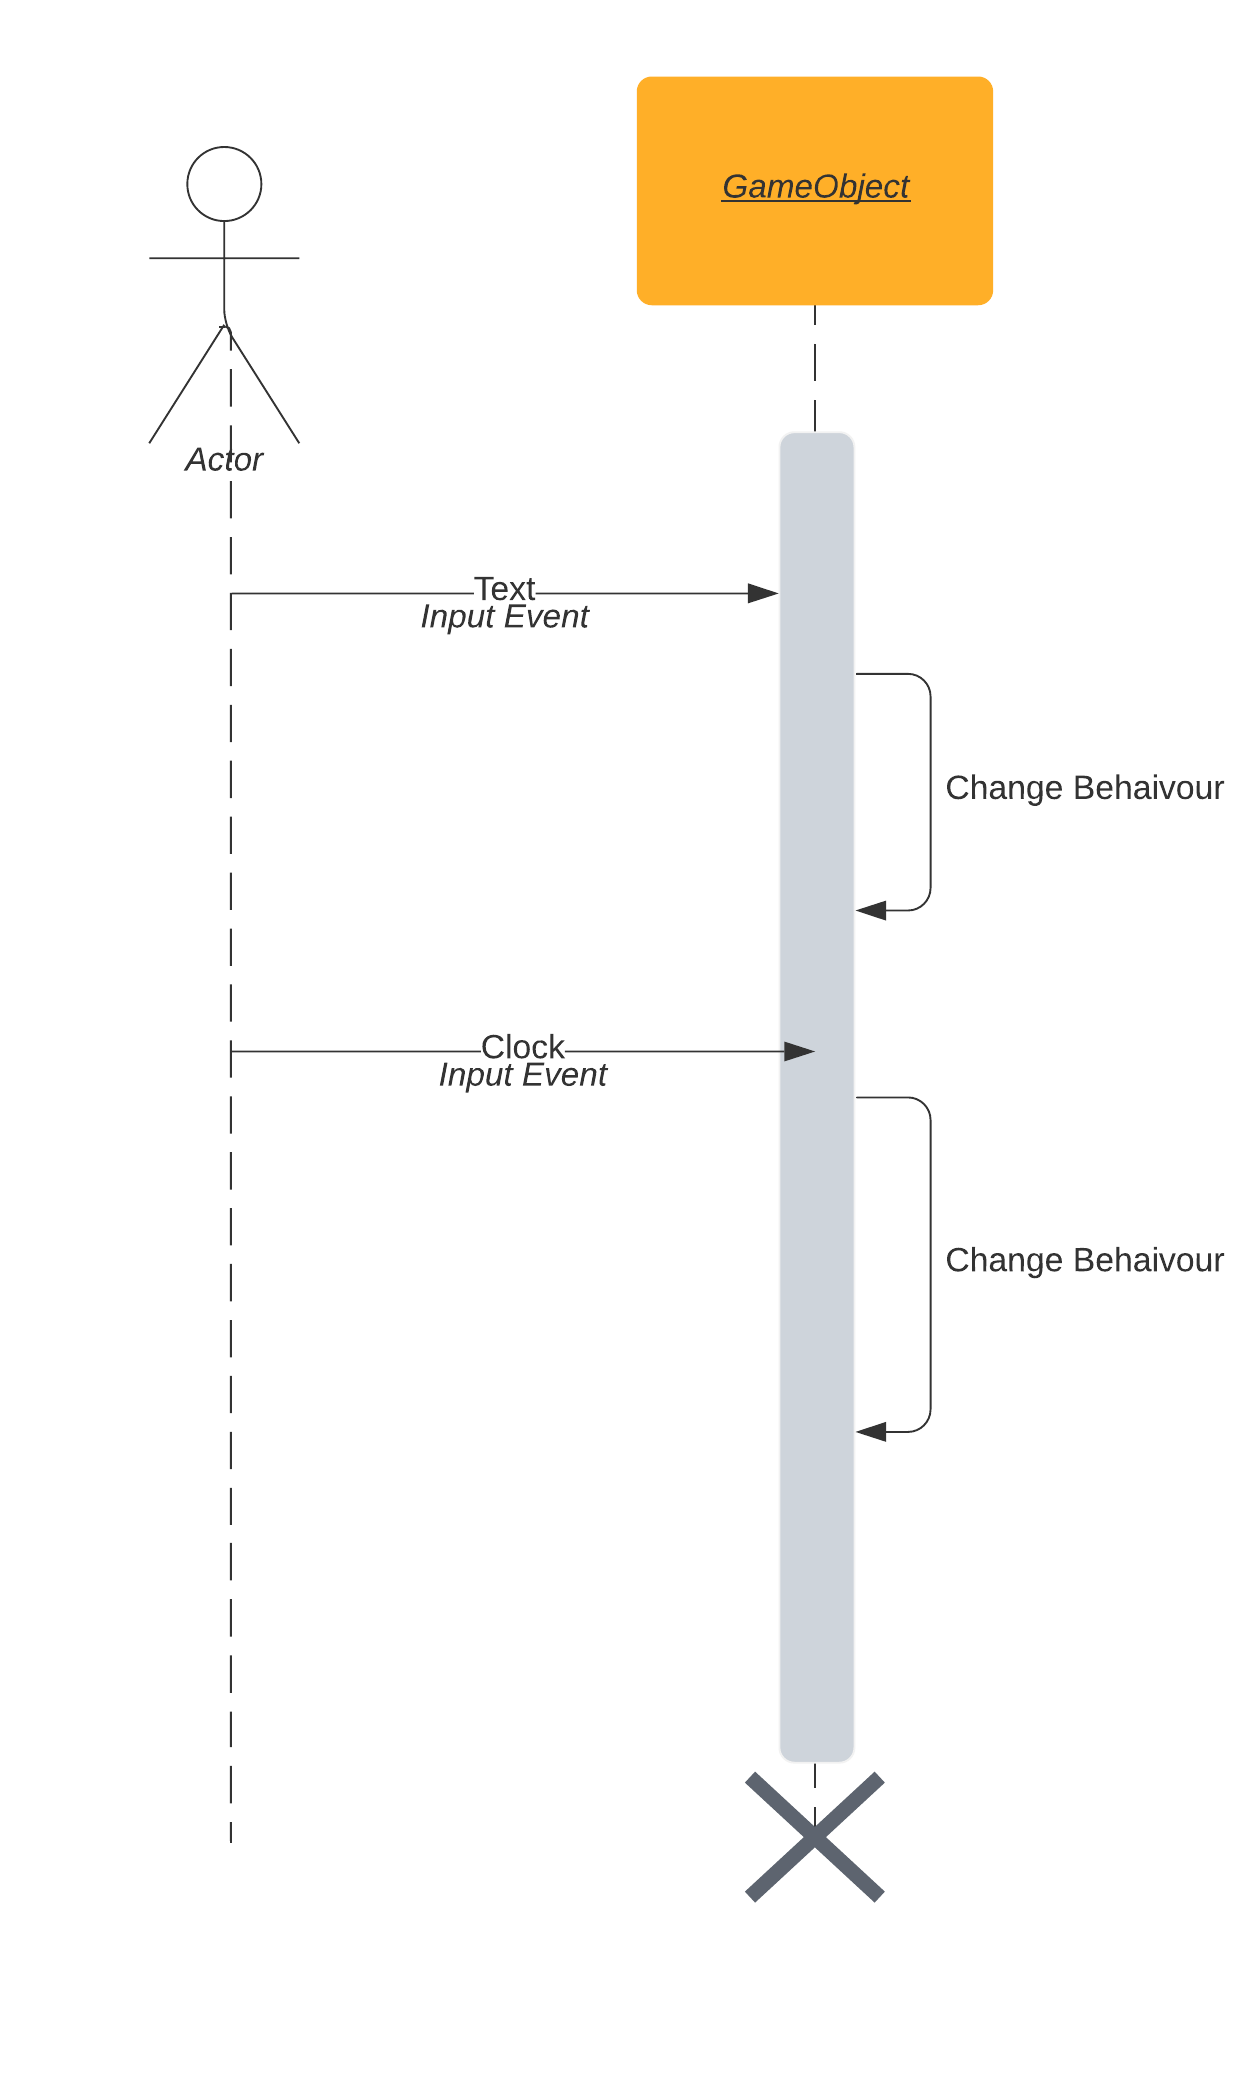
\includegraphics[scale=0.80, keepaspectratio]{img/UserEvent.png}
    \caption{Esquema de ejecución UML de eventos de teclado y reloj desde el usuario a cambio del comportamiento del objeto de juego}
    \label{figura:UserEvent}
\end{figure}

%%%%%%%%%%%%%%%%%%%%%%%%%%%%%%%%%%%%%%%%%%%%%%%%%%%%%%%%%%%%%%%%%%%%%%%%%%%%%%%%
%%%%%%%%%%%%%%%%%%%%%%%%%%%%%%%%%%%%%%%%%%%%%%%%%%%%%%%%%%%%%%%%%%%%%%%%%%%%%%%%
% RESULTADOS %
%%%%%%%%%%%%%%%%%%%%%%%%%%%%%%%%%%%%%%%%%%%%%%%%%%%%%%%%%%%%%%%%%%%%%%%%%%%%%%%%

\cleardoublepage
\chapter{Resultados}

En esta fase presentaremos algunas simulaciones realizadas con el motor con visualizaciones en OpenGL y realizaremos una comparativa
con el motor gráfico Blender mencionado en antecedentes y estado del arte en la simulación final del sistema solar.

\section{Simulaciones}
\label{sec:Simulaciones}

La primera simulación está compuesta por tres luces puntuales que iluminan diferentes partes de un cubo, las luces están situadas
en una posición cercana al cubo y contiene un factor de atenuación bajo. El cubo cuenta con una componente externa que permite
apagar y encender las luces pulsando una tecla. La componente externa tiene la lógica de un conmutador. Además el cubo rota sobre
sí mismo dentro de la escena para mostrar las diferentes partes del cubo iluminadas por la escena en la animación.

\begin{figure}[H]
    \centering
    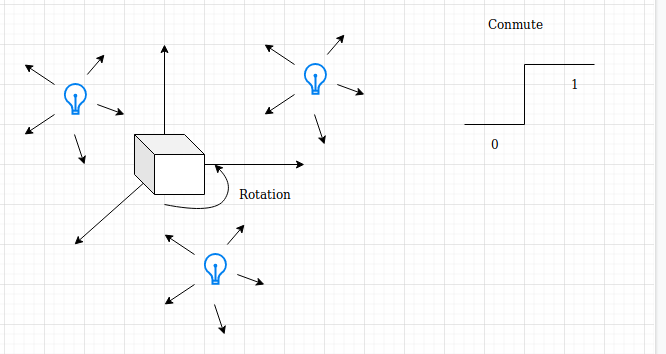
\includegraphics[scale=0.50, keepaspectratio]{img/SimpleCube.png}
    \caption{Ejemplo de uso de luces puntuales y eventos de teclado haciendo uso de las componentes externas del usuario.}
    \label{figura:SimpleCube}
\end{figure}

En esta simulación se muestran las ventajas del uso de las componentes externas para que el usuario del motor pueda realizar
cualquier tipo de simulación con total libertad de uso en el movimiento de los objetos, en el posicionamiento de las luces
puntuales y el uso del teclado para simular acciones sobre la escena.

\begin{figure}[H]
    \centering
    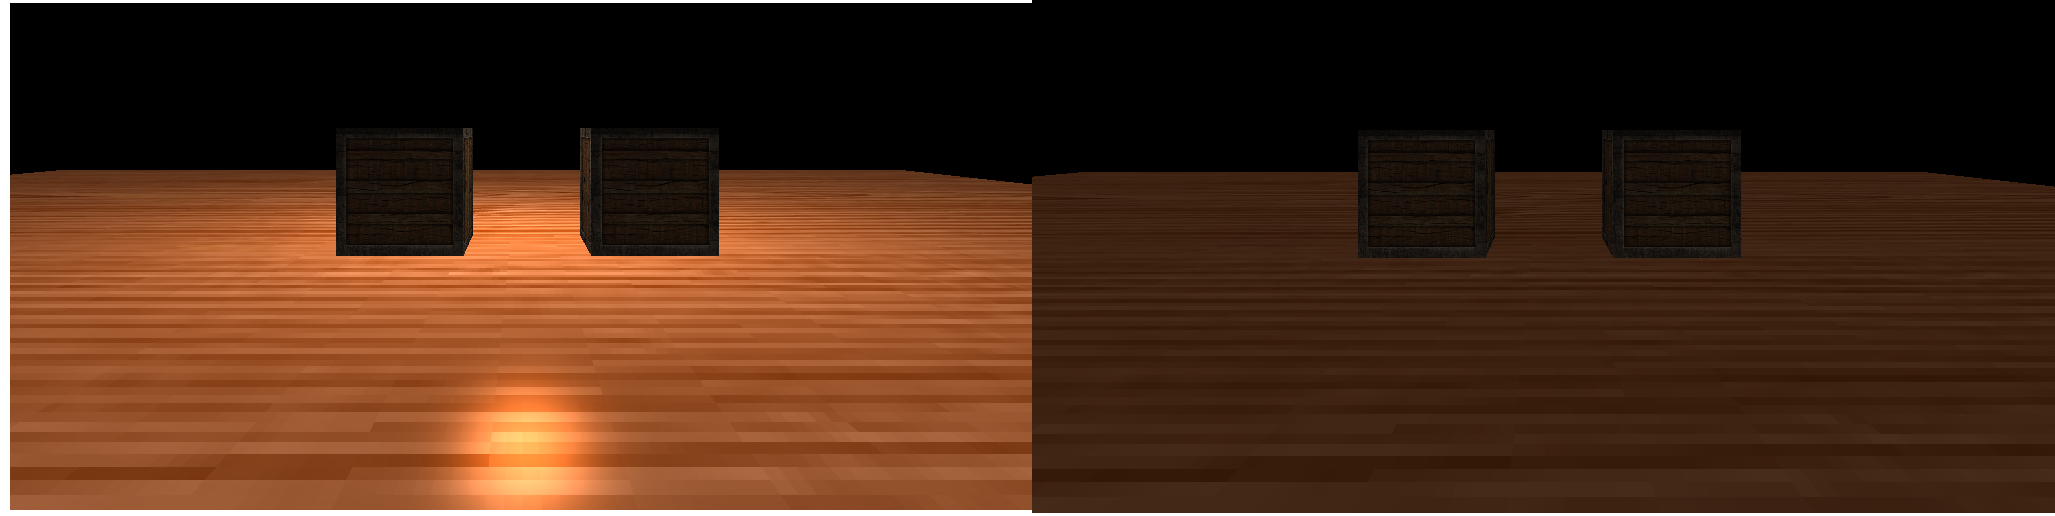
\includegraphics[scale=0.45, keepaspectratio]{img/CubeEvents.png}
    \caption{Imagen de la escena de cubos con la utilización del teclado para generar un cambio dinámico en la iluminación.}
    \label{figura:CubeEvents}
\end{figure}

En la figura 5.2 se puede observar la escena con un suelo y dos cajas y el cambio de iluminación de la luz puntual generado por
el pulso de una tecla por parte del usuario generando el apagado o el encendido de la luz dentro de la simulación.

\vspace{1mm} %5mm vertical space

La segunda simulación muestra el uso de las texturas normales en un plano y haciendo uso de una luz direccional para mostrar
el efecto de las texturas normales. El plano rota sobre sí mismo para ver el efecto de las componentes tangenciales de la
geometría y demostrar que al cambiar la dirección de incidencia de la luz sobre la superficie del plano el efecto de la textura
normal se mantiene, dando el efecto de rugosidad deseada sobre la superficie.

\begin{figure}[H]
    \centering
    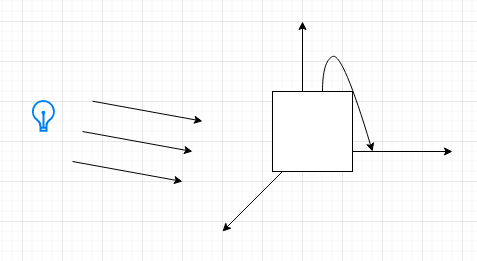
\includegraphics[scale=0.50, keepaspectratio]{img/WallDiagram.png}
    \caption{Esquema de la simulación del muro con texturas normales y uso de vectores tangenciales.}
    \label{figura:WallDiagram}
\end{figure}

A continuación se muestra la simulación del motor gráfico del uso de las texturas normales dentro del motor, haciendo uso de un
material especificado por el usuario para generar la superficie normal sobre el material.

\begin{figure}[H]
    \centering
    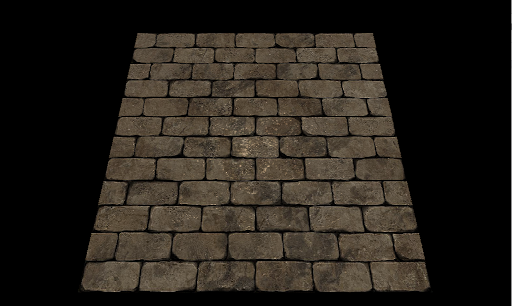
\includegraphics[scale=0.50, keepaspectratio]{img/WallResult.png}
    \caption{Imagen de la simulación de un muro haciendo uso de una textura normal simulando rugosidad en la superficie.}
    \label{figura:WallResult}
\end{figure}

En la siguiente simulación realizaremos una muestra completa del uso del árbol de transformadas, para ello realizaremos
una simulación del sistema solar, donde existen dependencias de movimiento entre los diferentes objetos dentro de la
animación. La luna realizará una rotación y una traslación alrededor de la tierra y la tierra alrededor del sol, otros
planetas como mercurio y marte rotarán también alrededor del sol. Existirá una luz puntual en el centro de la escena
simulando la  iluminación del sol y una luz direccional con una intensidad baja para no dejar completamente oscuras
las caras ocultas de la luna o los planetas.

\vspace{1mm} %5mm vertical space

Para realizar el movimiento de rotación y traslación del planeta tierra respecto al sol se deben realizar dos tipos de
movimientos diferentes, para ello se hará uso de dos transformadas. Un objeto de juego vacío con la transformada de
traslación del planeta y otra transformada donde estará almacenada la geometría encargada de la rotación.

\begin{figure}[H]
    \centering
    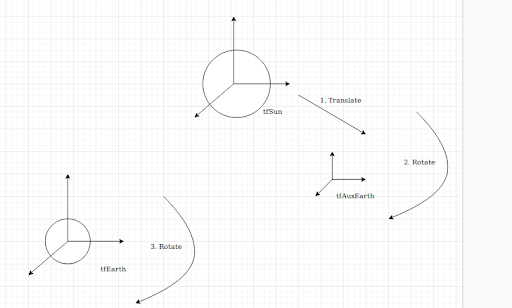
\includegraphics[scale=0.50, keepaspectratio]{img/SolarMove.png}
    \caption{Esquema de movimiento de traslación y rotación de los planetas del sistema solar}
    \label{figura:SolarMove}
\end{figure}

Como se puede ver en el ejemplo, la transformada auxiliar realiza dos operaciones de movimiento, un primer movimiento
de traslación y un segundo movimiento de rotación. Esta secuencia genera el movimiento de traslación de los planetas.
El segundo paso es la transformada de la geometría, esta transformada genera el movimiento de rotación del planeta.

\vspace{1mm} %5mm vertical space

Para realizar la dependencia de movimientos de rotación y traslación en la geometría se utiliza el árbol de transformadas
creado dentro del motor. En el caso del movimiento de la luna los pasos son los mismos pero en lugar de realizar la operación
respecto a la transformada del sol que coincide con la transformada raíz que define el valor absoluto de las posiciones de los
objetos en la escena. El movimiento de traslación y rotación se hace respecto a la transformada auxiliar del planeta tierra
que genera su traslación dentro del sistema solar. La tierra contará con el efecto de nubes que serán simuladas con el uso
de un objeto transparente, este objeto se sobre pondrá a la esfera de la tierra para que de la sensación de la atmósfera
terrestre sobre el planeta.

\begin{figure}[H]
    \centering
    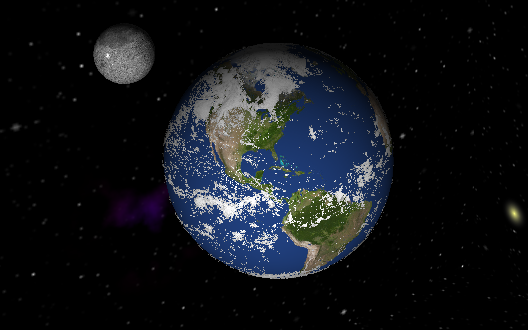
\includegraphics[scale=0.35, keepaspectratio]{img/Earth.png}
    \caption{Simulación del planeta tierra junto a la luna y el uso del objeto transparente para simular las nubes y su
    movimiento sobre el planeta.}
    \label{figura:Earth}
\end{figure}

En el caso de los demás planetas las acciones de movimiento son las mismas lo único que deberemos realizar de forma diferente
será el anillo de saturno ya que deberemos añadir un objeto no esférico dentro de la escena.

\vspace{1mm} %5mm vertical space

Para realizar el anillo de saturno cargaremos un toroide realizado en blender que se exportará en formato .obj dentro de la carpeta
de modelos del motor. Una vez cargado el anillo se añadirá la componente del anillo para generar movimiento o escalar el toroide
para que quede acorde con el tamaño del planeta, se añade al árbol de escena cómo hijo de la transformada auxiliar del planeta
saturno y el anillo queda en la misma posición del planeta completando el modelo completo que consta como podemos observar de
dos geometrías diferentes.

\begin{figure}[H]
    \centering
    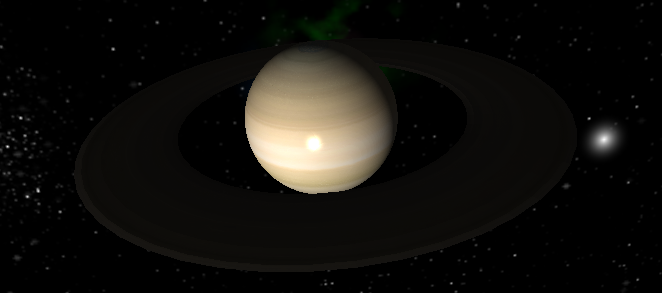
\includegraphics[scale=0.35, keepaspectratio]{img/saturno.png}
    \caption{Planeta Saturno compuesto de sus dos geometrías toroide simulando su anillo y esfera para simular el planeta.}
    \label{figura:saturno}
\end{figure}

Una vez posicionados los planetas y añadidas las traslaciones y rotaciones, el siguiente paso de la creación del entorno es generar
un fondo estelar haciendo uso del la técnica de skybox rodeando la textura a todos los planetas. Cada planeta cuenta con una
componente cámara añadida al objeto de esta manera es posible realizar el seguimiento de cada planeta de manera independiente.
Para terminar se muestra una visión general del sistema solar simulado con el motor gráfico desarrollado.

\begin{figure}[H]
    \centering
    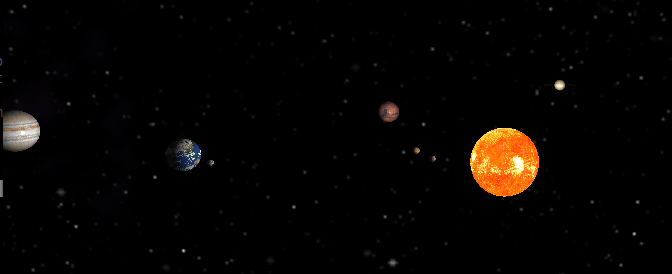
\includegraphics[scale=0.50, keepaspectratio]{img/SistemaSolar.png}
    \caption{Imagen del sistema solar mostrando los planetas desde mercurio hasta saturno.}
    \label{figura:Earth}
\end{figure}

En la imagen es posible observar los diferentes planetas del sistema solar y el efecto de la luz del sol sobre los planetas al igual que
el sol está completamente iluminado al diferenciarse de los demás planetas en que este objeto emite una fuente de luz y por tanto no está
compuesto por el mismo material que los planetas.

\vspace{1mm} %5mm vertical space

En la siguiente simulación veremos el uso de geometrías más complicadas exportadas en el motor con el uso de la librería Assimp del
motor gráfico. La simulación tratará un entorno virtual simulando un aeropuerto militar. La primera parte de la simulación será cargar
un avión o una torre de control como se puede comprobar en la siguiente imagen.

\begin{figure}[H]
    \centering
    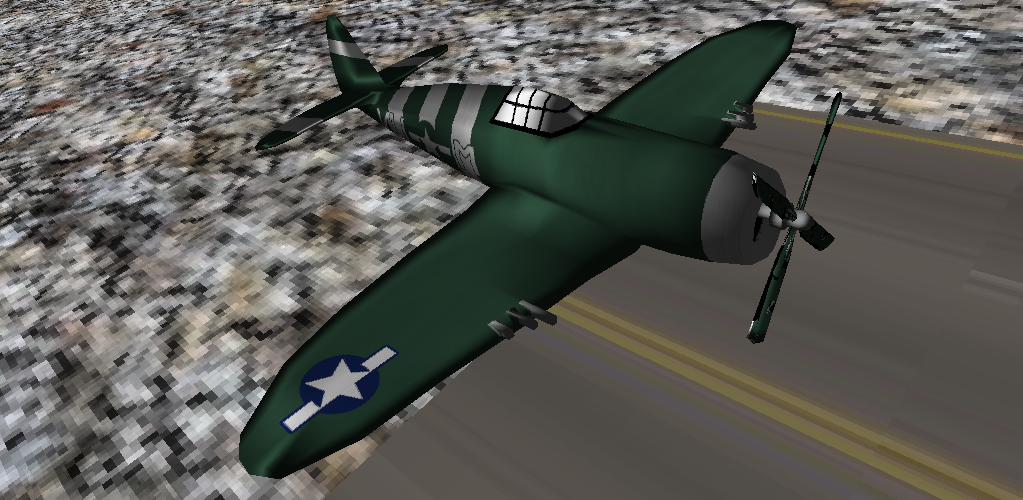
\includegraphics[scale=0.25, keepaspectratio]{img/Airplane.png}
    \caption{Ejemplo de carga de modelo geométrico avión de combate haciendo uso de la librería Assimp.}
    \label{figura:Avion}
\end{figure}

En la imagen se muestra el uso de la librería assimp del motor para realizar la carga de la geometría de un avión de combate con su
material correspondiente. La carga de la geometría se realiza a través de los ficheros .obj mientras que los materiales son cargados
en el motor en los ficheros .mtl. Además el usuario puede realizar la implementación de la reacción del material a la luz en los programas
de shaders.

\begin{figure}[H]
    \centering
    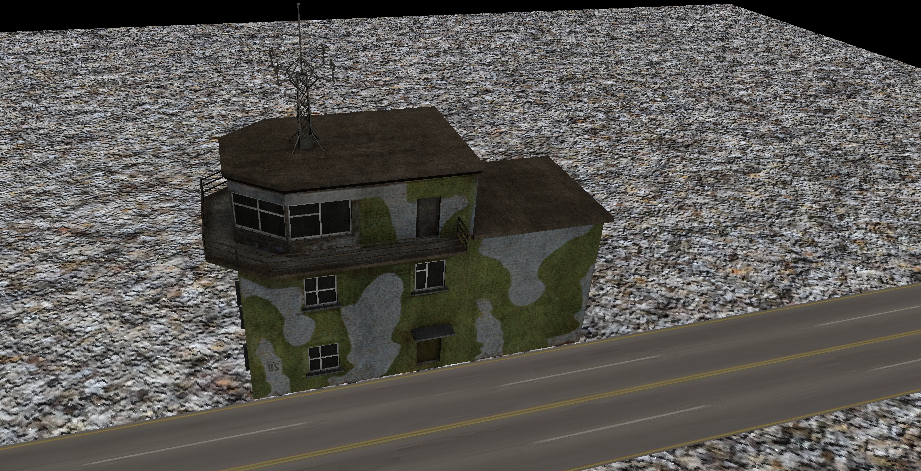
\includegraphics[scale=0.25, keepaspectratio]{img/Tower.png}
    \caption{Ejemplo de carga de modelo geométrico torre de control haciendo uso de la librería Assimp.}
    \label{figura:Avion}
\end{figure}

El entorno de la simulación de la torre de control y la pista de aterrizaje se puede hacer de igual manera. En este caso la pista de aterrizaje
utiliza un modelo de plano con una textura añadida de forma manual, mientras que la torre de control cuenta con una geometría y unas texturas
pre definidas en los ficheros .obj y .mtl del modelo.

\vspace{1mm} %5mm vertical space

Para acabar la simulación del aeropuerto se han añadido un fondo simulando el cielo y la utilización de diferentes objetos de juego para
simular un conjunto de aviones estacionados en pista haciendo uso del árbol de transformadas y las componentes externas de usuario.

\begin{figure}[H]
    \centering
    \includegraphics[scale=0.25, keepaspectratio]{img/AirportMultiplePlanes.png}
    \caption{Simulación de aeropuerto militar con Skybox y uso de las componentes externas y el árbol de transformadas para enseñar un
    conjunto de aviones de combate aparcados en el aeropuerto.}
    \label{figura:Avion}
\end{figure}

\section{Comparativas con Blender}
\label{sec:BlenderComp}

Para la simulación con blender se simulará un sistema solar realizado dentro de este motor gráfico haciendo uso de un árbol de transformadas,
uso de texturas difusas, animación con los script de python de blender y uso de luces y Skybox. 

\vspace{1mm} %5mm vertical space

Una vez realizada la  simulación se realizará una comparativa de los frames por segundo de ambos motores gráficos para ver a modo de
rendimiento quien obtiene mejores resultados haciendo uso del mismo hardware para la ejecución de ambas simulaciones.

\vspace{1mm} %5mm vertical space

Además veremos a modo de funcionalidad y características ambos motores para comprobar cual de los dos es más fácil de manejar a nivel
de usuario.

\subsection{Sistema solar con animación en Blender}
\label{subsec:BlenderComp}

En primer lugar se generarán las geometrías de las esferas para simular tanto el sol como los diferentes planetas. Una vez terminada
la geometría esférica de los planetas y el sol se distinguirá cada planeta por su material que tendrán adjuntados la textura de su
correspondiente superficie planetaria de esta manera se distinguirá las esferas como planetas del sistema solar. 

\begin{figure}[H]
    \centering
    \includegraphics[scale=0.25, keepaspectratio]{img/Geometry.png}
    \caption{Visualización de la geometría y sus primitivas de vértices de una esfera.}
    \label{figura:Geometry}
\end{figure}

En la figura 5.12 se puede ver las primitivas de vértices de la esfera, se ha realizado una subdivisión de los vértices para obtener una mayor
resolución de la superficie cuando el usuario acerque la cámara al planeta y no sean apreciables los triángulos en la superficie

\begin{figure}[H]
    \centering
    \includegraphics[scale=0.25, keepaspectratio]{img/MaterialBlender.png}
    \caption{Visualización de materiales en blender.}
    \label{figura:materialesBlender}
\end{figure}

En la figura 5.13 se visualiza la especificación de materiales en blender aplicando un shader de tipo difuso al que se le añade una
textura de tipo imagen de esta manera definimos la superficie del objeto con un material similar al usado en el proyecto. En blender
se puede especificar propiedades como el valor especular, el valor difuso que en nuestro caso hemos añadido como valor de color
de la superificie la textura de imagen.

\begin{figure}[H]
    \centering
    \includegraphics[scale=0.45, keepaspectratio]{img/SceneSolar.png}
    \caption{Visualización del árbol de escena en blender.}
    \label{figura:materialesBlender}
\end{figure}

En la figura 5.14 se observa el árbol de transformadas de la escena donde hemos añadido a la tierra cómo objeto hijo de una transformada
vacía a la que hemos llamado EarthAux similar a la utilizada en el proyecto. La transformada vacía EarthAux tiene como objeto padre el
sol, de esta manera podremos realizar el mismo movimiento de traslación realizado en el proyecto para la animación. 

\begin{figure}[H]
    \centering
    \includegraphics[scale=0.20, keepaspectratio]{img/Scripting.png}
    \caption{Visualización de scripting de la API de python para blender para generar movimientos.}
    \label{figura:materialesBlender}
\end{figure}

En la figura 5.15 se observa el uso de la API de python de blender Blender Python, esta API permite al desarrollador acceder a los objetos de la
escena y a sus matrices global y local, con el acceso a las matrices de los objetos se pueden realizar los movimientos de rotación y
traslación haciendo uso del árbol de transformadas modificando el valor de la matriz local de modelo y de esta manera mantener las
dependencias de las posiciones del árbol.

\begin{figure}[H]
    \centering
    \includegraphics[scale=0.45, keepaspectratio]{img/AnimationBlender.png}
    \caption{Visualización de la animación de movimiento de la tierra alrededor del sol.}
    \label{figura:materialesBlender}
\end{figure}

En la figura 5.16 se presenta la animación de la escena de la tierra alrededor del sol la parte de abajo de ventanas de blender
muestra el frame actual de la animación la barra amarilla muestra los registros de movimientos del objetos EarthAux y Earth en
la simulación el movimiento de rotación de la tierra y traslación se puede observar en los dos pasos de la imagen con dos
capturas diferentes en dos frames diferentes.

\begin{figure}[H]
    \centering
    \includegraphics[scale=0.25, keepaspectratio]{img/MoonAux.png}
    \caption{Ejemplo de uso del árbol de transformadas en blender para el movimiento de la luna.}
    \label{figura:materialesBlender}
\end{figure}

Para realizar el movimiento de la luna se realiza el mismo procedimiento que para la tierra pero añadiendo la transformada de la
luna y su transformada auxiliar objetos hijos de la transformada auxiliar de la tierra dando el resultado de la figura 5.17

\vspace{1mm} %5mm vertical space

La siguiente parte a definir una vez visto el árbol de transformadas la definición de las primitivas de la esfera y su material con
una textura basada en imagen es aplicar un Skybox desde blender para ello se siguen dos etapas diferentes añadir el cubo y definir
las coordenadas de texturas para el cubo y definir el material del Skybox.

\begin{figure}[H]
    \centering
    \includegraphics[scale=0.65, keepaspectratio]{img/SkyBoxBlender.png}
    \caption{Visualización de la definición de vértices del cubo para generar el SkyBox y las coordenadas de textura correspondiente.}
    \label{figura:materialesBlender}
\end{figure}

En esta figura se puede observar cómo se ha definido de forma manual el orden de alineación de los vértices de la geometría esta
modificación permitirá en el siguiente paso añadir una textura de Skybox a la geometría ya que hemos modificado como están
ordenadas las coordenadas de textura.

\begin{figure}[H]
    \centering
    \includegraphics[scale=0.65, keepaspectratio]{img/SkyBoxVertex.png}
    \caption{Redefinición de las coordenadas de textura del cubo para añadir una textura de Skybox a la geometría.}
    \label{figura:materialesBlender}
\end{figure}

En este paso se añade la imagen que se quiere añadir cómo SkyBox una vez añadida la textura se debe redefinir las coordenadas
de textura del cubo para que cuadren con la imagen y de esta manera añadir la textura como material y cuadre de forma correcta
con las caras del cubo, por último se añade un material al cubo con una textura con la imagen definiendo de esta manera las
superficies del cubo.

\begin{figure}[H]
    \centering
    \includegraphics[scale=0.25, keepaspectratio]{img/SkyBoxFinal.png}
    \caption{Redefinición de las coordenadas de textura del cubo para añadir una textura de Skybox a la geometría.}
    \label{figura:materialesBlender}
\end{figure}

Se puede observar el resultado del Skybox dentro de la escena a forma de paisaje en segundo plano de una nebulosa dentro
del sistema solar. Estas son las partes básicas del motor gráfico blender utilizadas para realizar una simulación parecida
al sistema solar utilizado en el motor gráfico desarrollado dentro del proyecto. 

\vspace{1mm} %5mm vertical space

En la siguiente parte de la memoria se realiza una serie de medidas de rendimiento y comparativas de funcionalidad entre
blender y el motor gráfico desarrollado.

\section{Comparativas de funcionalidad y rendimiento}
\label{sec:CompEngine}

Este apartado muestra la funcionalidad desarrollada en el proyecto para consolidar que estas funcionalidades son comunes en
el uso de motores gráficos:

\begin{enumerate}
  \item La generación de un árbol de transformadas es utilizado también en blender para realizar el posicionamiento de
  los objetos dentro de la escena de renderizado.

  \item La utilización de shaders o materiales es utilizada también en ambos motores, haciendo uso de texturas para
  describir las superficies de los objetos gráficos.
  
  \item Realización de animaciones a través de lenguaje de programación haciendo uso de una API del motor gráfico.
  Blender además de contar con la GUI puede realizar todas las operaciones del motor a través de su API gráfica BPY. 
  El motor gráfico del proyecto cuenta con una API para realizar las escenas animaciones y definición de los objetos.

  \item La capacidad de realizar entornos a través de skybox es posible en blender aunque es una tarea mucho más 
  complicada que la desarrollada en el proyecto.

  \item Blender es capaz de importar y exportar geometrías con la definición de los materiales de un objeto gráfico,
  el motor del proyecto es capaz de importar esta clase de objetos y realizar un renderizado de forma sencilla.

  \item El uso de la iluminación en blender se realiza a través de diferentes tipos de luz que reflejan el material
  según sus propiedades, el motor gráfico desarrollado cuenta con tres tipos de luces que pueden ser animadas dentro
  de la escena.

  \item Blender cuenta con cámaras ortográficas para entornos 2D y cámaras de perspectiva para realizar renderizaciones
   en 3D, el motor gráfico desarrollado puede crear ambos tipos de cámara a través de sus propiedades.

  \item Uso de controlador de cámara, a partir de la API en blender es posible realizar un movimiento de cámara dentro
  de la animación configurando qué teclas se utilizan para mover la cámara, al igual que en el motor gráfico del proyecto.

\end{enumerate}

Blender cuenta con muchas otras funcionalidades no investigadas en el proyecto, ya que se trata de un motor gráfico profesional,
sin embargo las funcionalidades desarrolladas en el proyecto cumplen los objetivos mínimos de funcionalidades del motor gráfico de blender.

\vspace{1mm} %5mm vertical space

La siguiente parte del capítulo muestra las medidas de rendimiento obtenidas en ambos motores con simulaciones de un sistema
solar parecido y con la misma limitación de imágenes por segundo.

\subsection{Medidas de rendimiento}

Para realizar las comparativas de rendimiento hemos utilizado dos simulaciones del sistema solar parecidas en ambos motores hasta
encontrar diferencias significativas en el rendimiento  dentro de la misma máquina. 

\begin{figure}[H]
    \centering
    \includegraphics[scale=0.25, keepaspectratio]{img/FPSBlender.png}
    \caption{Gráfica de rendimiento de motor gráfico blender durante la animación del sistema solar}
    \label{figura:materialesBlender}
\end{figure}

La primera medida de rendimiento muestra el sistema solar renderizado por blender donde se puede observar que se llega al máximo de
imágenes por segundo a las que está limitado el motor sin embargo es bastante inestable mientras avanza la animación, ya que hay
picos de bajada de imágenes de hasta diez o veinte imágenes, esto es apreciable por el usuario a la hora de ver la renderización
de su escena.

\begin{figure}[H]
    \centering
    \includegraphics[scale=0.50, keepaspectratio]{img/FPSEngine.png}
    \caption{Gráfica de rendimiento de motor gráfico del proyecto durante la simulación del sistema solar}
    \label{figura:materialesBlender}
\end{figure}

En la segunda gráfica de rendimiento se muestra las medidas realizadas sobre el motor gráfico del proyecto, en este segundo
caso se puede observar una mayor estabilidad en la cantidad de imágenes generadas por segundo durante la renderización
aunque no se llegue a obtener el máximo de FPS configurado dentro del motor gráfico por la carga de trabajo.

%%%%%%%%%%%%%%%%%%%%%%%%%%%%%%%%%%%%%%%%%%%%%%%%%%%%%%%%%%%%%%%%%%%%%%%%%%%%%%%%
%%%%%%%%%%%%%%%%%%%%%%%%%%%%%%%%%%%%%%%%%%%%%%%%%%%%%%%%%%%%%%%%%%%%%%%%%%%%%%%%
% CONCLUSIONES %
%%%%%%%%%%%%%%%%%%%%%%%%%%%%%%%%%%%%%%%%%%%%%%%%%%%%%%%%%%%%%%%%%%%%%%%%%%%%%%%%

\cleardoublepage
\chapter{Conclusiones}
\label{chap:conclusiones}


\section{Consecución de objetivos}
\label{sec:consecucion-objetivos}

En la realización del proyecto se ha conseguido realizar de forma existosa, la funcionalidad básica de un motor gráfico orientado
a realizar aplicaciones gráficas capaces de realizar operaciones interactivas con el usuario. Entre los objetivos definidos se ha
conseguido realizar las siguientes tareas:

\begin{enumerate}
  \item Realizacion de un motor gráfico con renderización de objetos en 3D, simulación de luces y movimiento de los objetos
  \item Importación de objetos geométricos complejos a partir de un formato estándar .obj
  \item Realización de eventos dentro de la animación con el uso del teclado y reloj
  \item Utilización de una API gráfica de alto nivel para realizar las simulaciones gráficas a partir de componentes.
  \item Definición de materiales de manera dinámica donde el usuario decide las propiedes de los modelos que cargue en el motor.
  \item Comparación con otros motóres gráficos dentro de la industria de los videojuegos y animación, incluyendo medidas de 
  rendimiento utilizadas en las aplicaciones gráficas en la renderización.
\end{enumerate}

El motor cumple con los módulos gráficos básicos para realizar simulaciones virtuales interactivas, aunque la parte de comparativas haya
quedado simplificado por la complejidad de la curva de aprendizaje de los motores gráficos sin experiencia previa, se ha conseguido realizar
una simulación dentro de Blender que muestra las funcionalidades desarrolladas en el proyecto. 

\vspace{1mm} %5mm vertical space

El trabajo admeás ha servido para aprender las partes básicas de funcionamiento de un motor gráfico a través de la interfaz gráfica OpenGL, 
incluyendo el estudio de otras interfáces gráficas actuales, Vulkan y DirectX y la decisión del uso de la API gráfica de OpenGL, para
la comunicación del desarrollador con la GPU para el programación de gráficos.

\vspace{1mm} %5mm vertical space

El proyecto también a servido para enseñar al alumno las abstracciones más comunes dentro de un motor gráfico, modelos, geometrías, materiales
o tipos de luces, con un modelo de iluminación y el estudio de un motor gráfico para justificar el desarrollo de los módulos del motor 
gráfico desarrollado.

\section{Trabajos futuros}
\label{sec:trabajos_futuros}

\subsubsection{Uso de instanciación}

Para mejorar el rendimiento del motor gráfico, se puede realizar el uso de la instanciación, este método de renderizado
permite replicar una misma geometría sin hacer uso de la comunicación continua de la CPU con la GPU, realizando el cauce
gráfico para estas múltiples geometrías homogéneas en una única estructura de datos en forma de array. El motor gráfico
debería tener en cuenta la posibilidad de renderizar el mismo objeto con un contador de número de veces de replicación.
Al obtener el número de objetos a renderizar el usuario podría hacer uso de la API gráfica para definir los materiales
de cada objeto de forma específica indicando el material de cada geometría.

\vspace{1mm} %5mm vertical space

En el caso de la simulación del sistema solar o la simulación de aviones este método reduciría la carga de trabajo entre
la CPU y la GPU optimizando de forma significativa el rendimiento del motor.

\begin{figure}[H]
    \centering
    \includegraphics[scale=0.40, keepaspectratio]{img/instanciacint_asteroids.png}
    \caption{Ejemplo de instanciación de los asteroides del anillo de Saturno en Learn OpenGL.}
    \label{figura:materialesBlender}
\end{figure}

\subsubsection{Post procesamiento}

Otra característica a añadir dentro del motor gráfico es el uso del postprocesado. Esta característica permite
al desarrollador manejar la renderización final como si fuera una textura. Al realizar esta operación dentro del
contexto de OpenGL se puede realizar operaciones sobre la imagen final con técnicas de procesado de imágenes, cómo
inversión de color, filtrado de bordes o realización de desenfoque de la imagen. Actualmente el motor gráfico utiliza
el buffer de renderización por defecto de OpenGL, este buffer realiza las operaciones del cauce gráfico y en el
momento de realizar la etapa de rasterización almacena la información de los fragmentos en este buffer por defecto.
El uso de un framebuffer específico permite realizar operaciones en el buffer de renderizado una vez se ha almacenado
con los datos de los fragmentos.

\vspace{1mm} %5mm vertical space

El resultado final es una textura con los datos de los fragmentos que puede ser utilizada para realizar las operaciones
sobre las imágenes explicadas anteriormente.

\begin{figure}[H]
    \centering
    \includegraphics[scale=0.35, keepaspectratio]{img/framebuffers_inverse.png}
    \caption{Realización de operación de imagen inversa. 1 - x.}
    \label{figura:materialesBlender}
\end{figure}

Una de las operaciones realizadas en el uso del post procesado en la etapa de fragmentos sobre la textura de la pantalla
es realizar el valor negativo de los colores de la imagen. Otro uso muy utilizado en procesamiento de imágenes es el uso
de kernels, estas matrices de 3x3 permite realizar operaciones de convolución sobre la imagen realizando la detección de
bordes o el desenfoque de las imágenes.

\begin{equation} \label{distance}
    Imagen_{final} = Imagen_{screen} * Kernel
\end{equation}

\begin{figure}[H]
    \centering
    \includegraphics[scale=0.35, keepaspectratio]{img/PostProcessing.png}
    \caption{Muestra del uso de procesado de imagen para detección de bordes y desenfoque.}
    \label{figura:materialesBlender}
\end{figure}

Las matrices 3x3 de kernel tienen valores conocidos y son utilizados para obtener el efecto deseado sobre la imagen final 
de renderizado, en este caso la imagen muestra un procesado para detección de bordes y desenfoque. Estas operaciones son
muy utilizadas en aplicaciones de imagen como photoshop donde las operaciones sobre los pixeles son fácilmente paralelizables
ya que cada pixel de la imagen se procesa de manera independiente haciendo fácil el uso de las tarjetas gráficas para este
tipo de operaciones.


\section{Valoración personal}
\label{sec:valoracion}

Este trabajo trata de explicar los módulos básicos necesarios dentro de un motor capaz de realizar aplicaciones gráficas
interactivas y simulación de un mundo animado. El trabajo intenta explicar cómo funcionan este tipo de plataformas que utilizan
las interfaces de las tarjetas gráficas para el procesamiento de video. El trabajo está formado por las partes más sencillas
importantes para un comienzo de proyecto de motor gráfico utilizando la librería gráfica OpenGL y mostrando al lector los
pasos a seguir para realizar un motor gráfico sencillo.

\vspace{1mm} %5mm vertical space

Las realizaciones de comparativas con otro motores gráficos a resultado un trabajo complicado debido a la inexperiencia en
este campo por parte del alumno, aunque se ha realizado una comparativas de rendimientos entre un motor gráfico profesional
y un motor gráfico del proyecto, lo más importante es comprobar que el motor gráfico del proyecto cumple con funcionalidades
similares a la de un motor gráfico profesional.


%%%%%%%%%%%%%%%%%%%%%%%%%%%%%%%%%%%%%%%%%%%%%%%%%%%%%%%%%%%%%%%%%%%%%%%%%%%%%%%%
%%%%%%%%%%%%%%%%%%%%%%%%%%%%%%%%%%%%%%%%%%%%%%%%%%%%%%%%%%%%%%%%%%%%%%%%%%%%%%%%
% APÉNDICE(S) %
%%%%%%%%%%%%%%%%%%%%%%%%%%%%%%%%%%%%%%%%%%%%%%%%%%%%%%%%%%%%%%%%%%%%%%%%%%%%%%%%

%%%%%%%%%%%%%%%%%%%%%%%%%%%%%%%%%%%%%%%%%%%%%%%%%%%%%%%%%%%%%%%%%%%%%%%%%%%%%%%%
%%%%%%%%%%%%%%%%%%%%%%%%%%%%%%%%%%%%%%%%%%%%%%%%%%%%%%%%%%%%%%%%%%%%%%%%%%%%%%%%
% BIBLIOGRAFIA %
%%%%%%%%%%%%%%%%%%%%%%%%%%%%%%%%%%%%%%%%%%%%%%%%%%%%%%%%%%%%%%%%%%%%%%%%%%%%%%%%

\cleardoublepage

% Las siguientes dos instrucciones es todo lo que necesitas
% para incluir las citas en la memoria

\bibliographystyle{apalike}
\bibliography{memoria}

\nocite{*}

% memoria.bib es el nombre del fichero que contiene
% las referencias bibliográficas. Abre ese fichero y mira el formato que tiene,
% que se conoce como BibTeX. Hay muchos sitios que exportan referencias en
% formato BibTeX. Prueba a buscar en http://scholar.google.com por referencias
% y verás que lo puedes hacer de manera sencilla.
% Más información: 
% http://texblog.org/2014/04/22/using-google-scholar-to-download-bibtex-citations/

\end{document}
